\documentclass[a4paper,UKenglish,cleveref, autoref, thm-restate,anonymous]{lipics-v2021}
%This is a template for producing LIPIcs articles. 
%See lipics-v2021-authors-guidelines.pdf for further information.
%for A4 paper format use option "a4paper", for US-letter use option "letterpaper"
%for british hyphenation rules use option "UKenglish", for american hyphenation rules use option "USenglish"
%for section-numbered lemmas etc., use "numberwithinsect"
%for enabling cleveref support, use "cleveref"
%for enabling autoref support, use "autoref"
%for anonymousing the authors (e.g. for double-blind review), add "anonymous"
%for enabling thm-restate support, use "thm-restate"
%for enabling a two-column layout for the author/affilation part (only applicable for > 6 authors), use "authorcolumns"
%for producing a PDF according the PDF/A standard, add "pdfa"

%\pdfoutput=1 %uncomment to ensure pdflatex processing (mandatatory e.g. to submit to arXiv)
%\hideLIPIcs  %uncomment to remove references to LIPIcs series (logo, DOI, ...), e.g. when preparing a pre-final version to be uploaded to arXiv or another public repository

%\graphicspath{{./graphics/}}%helpful if your graphic files are in another directory


\usepackage{amsmath}
%\let\proof\relax
%\let\endproof\relax

\sloppy


\usepackage{amsthm}
\usepackage{amssymb}
\usepackage{amsfonts}
\usepackage{mathrsfs}
\usepackage{wrapfig} %wrap the text around the picture


\usepackage{thmtools} 
\usepackage{thm-restate}

\usepackage{caption} %for subfigure - join multiple figures and add captions
\usepackage{subcaption}
\usepackage{changepage} %inside figure we can put \begin{adjustwidth}{-1cm}{-1cm} \end{adjustwidth} and we can ignore the margins
\usepackage{mathtools} % write text [under]{over} arrow $\xrightarrow[\text{world}]{\text{hello}}$

\usepackage{graphicx}
\graphicspath{{Figures/}}

\usepackage{tikz}

\usetikzlibrary{arrows,decorations.pathmorphing,decorations.pathreplacing,backgrounds,positioning,fit,matrix}
\usetikzlibrary{shapes,calc,patterns,arrows.meta}
\tikzset{
	vert/.style={circle,inner sep=1.5,fill=white,draw,minimum size=.3cm},
	edge/.style={color=black, thick},
	diredge/.style={->,>={Stealth[width=8pt,length=8pt]},color=black, thick},
	timelabel/.style={fill=white,font=\footnotesize, text centered},
	wave/.style={decorate,decoration={coil,aspect=0}},
	dirwave/.style={->, >={Stealth[width=8pt,length=8pt]},decorate,decoration={coil,aspect=0}},
	diredge2/.style={->,>={Stealth[width=8pt,length=8pt]}}
}

%\usepackage{enumitem} %enumerate 
\usepackage{enumerate}
\usepackage{todonotes}
\newcommand{\todonkl}[2][]{\todo[color=red!100!green!33,#1]{NKL:\\ #2}} %todo note that starts with NKL:
\setlength{\marginparwidth}{3.7cm} %setting the length of todonote


\usepackage{comment}

\usepackage{algorithm}
\usepackage[noend]{algpseudocode}


%font encoding
\usepackage[T1]{fontenc}
\usepackage[utf8]{inputenc}
\usepackage{lmodern}

\usepackage{hyperref}

\crefname{claim}{Claim}{Claims}

%\usepackage{natbib}

\newcommand{\ie}{i.\,e.,\ }
\renewcommand{\st}{s.\,t.,\ }
\newcommand{\NP}{\textrm{NP}}
\newcommand{\APX}{\textrm{APX}}
\newcommand{\FPT}{\textrm{FPT}}
\newcommand{\XP}{\textrm{XP}}

\newcommand{\NN}{\mathbb{N}}
\newcommand{\ZZ}{\mathbb{Z}}
\newcommand{\RR}{\mathbb{R}}
\newcommand{\QQ}{\mathbb{Q}}


%%%%%%%%%%%%%%%%%%%%%%%%%%%%%%%% Defining a problem
%%%%%%%%%%%%%%%%%%\problemdef{NAME} {Input} {Output}
\usepackage{tabularx}
\newcommand{\problemdef}[3]{
	\begin{center}
		\begin{minipage}{0.95\textwidth}
			\noindent
			#1
			\vspace{5pt}\\
			\setlength{\tabcolsep}{3pt}
			\begin{tabularx}{\textwidth}{@{}lX@{}}
				\textbf{Input:}& #2 \\
				\textbf{Question:}& #3
			\end{tabularx}
		\end{minipage}
	\end{center}
}

\newcounter{guesscounter}


%%%%%%%%%%%%%%%%%%%%%%%%%%%%%%%%%% PROBLEMS NAMES
%% One label per edge, period Delta, exact realization
\newcommand{\deltaExactLong}{\textsc{Simple periodic Temporal Graph Realization}}
\newcommand{\deltaExact}{\textsc{Simple TGR}}

%% k labels per edge, period Delta, exact realization
\newcommand{\kDeltaExactLong}{\textsc{$(k,\Delta)$-periodic Exact Temporal Graph Realization}}
\newcommand{\kDeltaExact}{\textsc{$(k,\Delta)$-TGR}}

%% One label per edge, period Delta, upper-bounded realization
\newcommand{\kDeltaUpperBoundLong}{\textsc{Simple $\Delta$-periodic Upper-Bounded Temporal Graph Realization}}
%\newcommand{\deltaUpperBound}{}

%% k labels per edge, period Delta, lower-bound realization
\newcommand{\kDeltaLowerBoundLong}{\textsc{Simple $\Delta$-periodic Lower-Bounded Temporal Graph Realization}}


\bibliographystyle{plainurl}% the mandatory bibstyle

\title{Realizing temporal graphs from fastest travel times} %TODO Please add

%\titlerunning{Dummy short title} %TODO optional, please use if title is longer than one line

%\author{Nina Klobas}{Department of Computer Science, Durham University, UK}{nina.klobas@durham.ac.uk}{ https://orcid.org/0000-0002-8024-5782}{}

%\author{George B. Mertzios}{Department of Computer Science, Durham University, UK}{george.mertzios@durham.ac.uk}{https://orcid.org/0000-0001-7182-585X}{Supported by the EPSRC grant EP/P020372/1.}

%\author{Hendrik Molter}{Department of Industrial Engineering and Management, Ben-Gurion~University~of~the~Negev, Israel}{molterh@post.bgu.ac.il}{https://orcid.org/0000-0002-4590-798X}{Supported by the ISF, grant No.~1070/20.}

%\author{Paul G. Spirakis}{Department of Computer Science, University of Liverpool, UK}{p.spirakis@liverpool.ac.uk}{https://orcid.org/0000-0001-5396-3749}{Supported by the EPSRC grant EP/P02002X/1.}

%\authorrunning{Nina Klobas, George B. Mertzios, Hendrik Molter, and Paul G. Spirakis} %TODO mandatory. First: Use abbreviated first/middle names. Second (only in severe cases): Use first author plus 'et al.'

%\Copyright{Nina Klobas, George B. Mertzios, Hendrik Molter, and Paul G. Spirakis} %TODO mandatory, please use full first names. LIPIcs license is "CC-BY";  http://creativecommons.org/licenses/by/3.0/

\ccsdesc[500]{Theory of computation~Graph algorithms analysis}
\ccsdesc[500]{Mathematics of computing~Discrete mathematics}
%TODO mandatory: Please choose ACM 2012 classifications from https://dl.acm.org/ccs/ccs_flat.cfm 

\keywords{Temporal graph, periodic temporal labeling, fastest temporal path, graph realization, temporal connectivity.} %TODO mandatory; please add comma-separated list of keywords

\category{} %optional, e.g. invited paper

\relatedversion{} %optional, e.g. full version hosted on arXiv, HAL, or other respository/website
%\relatedversiondetails[linktext={opt. text shown instead of the URL}, cite=DBLP:books/mk/GrayR93]{Classification (e.g. Full Version, Extended Version, Previous Version}{URL to related version} %linktext and cite are optional

%\supplement{}%optional, e.g. related research data, source code, ... hosted on a repository like zenodo, figshare, GitHub, ...
%\supplementdetails[linktext={opt. text shown instead of the URL}, cite=DBLP:books/mk/GrayR93, subcategory={Description, Subcategory}, swhid={Software Heritage Identifier}]{General Classification (e.g. Software, Dataset, Model, ...)}{URL to related version} %linktext, cite, and subcategory are optional

%\funding{(Optional) general funding statement \dots}%optional, to capture a funding statement, which applies to all authors. Please enter author specific funding statements as fifth argument of the \author macro.

%\acknowledgements{I want to thank \dots}%optional

%\nolinenumbers %uncomment to disable line numbering



%Editor-only macros:: begin (do not touch as author)%%%%%%%%%%%%%%%%%%%%%%%%%%%%%%%%%%
\EventEditors{John Q. Open and Joan R. Access}
\EventNoEds{2}
\EventLongTitle{42nd Conference on Very Important Topics (CVIT 2016)}
\EventShortTitle{CVIT 2016}
\EventAcronym{CVIT}
\EventYear{2016}
\EventDate{December 24--27, 2016}
\EventLocation{Little Whinging, United Kingdom}
\EventLogo{}
\SeriesVolume{42}
\ArticleNo{23}
%%%%%%%%%%%%%%%%%%%%%%%%%%%%%%%%%%%%%%%%%%%%%%%%%%%%%%














\begin{document}
\maketitle

\begin{abstract}
In this paper we study \emph{temporal design} problems of undirected temporally connected graphs. 
The basic setting of these optimization problems is as follows: given an undirected graph~$G$, 
what is the smallest number $|\lambda|$ of time-labels that we need to add to the edges of $G$ such that the resulting temporal graph $(G,\lambda)$ is temporally connected? 


\vspace{0,2cm}
\noindent \textbf{Due to lack of space, the full paper with all proofs is attached in a 
	clearly marked Appendix to be read at the discretion of the Program Committee.}
\end{abstract}


\section{Introduction}\label{intro-sec}

Graph realization problems are fundamental graph-algorithmic questions where the objective is to (re)construct a graph, 
given some constraints on some of its graph attributes. Among the most well studied such parameters for graph reconstruction 
are the vertex degrees~\cite{}, distances~\cite{}, eccentricities~\cite{}, connectivity~\cite{}, etc. 
The motivation for network realization problems stems from both ``verification'' applications where we attempt to reconstruct an existing network of unknown structure based on the outcomes of experimental measurements, and engineering applications related to network design~\cite{.....}. 

SKELETON:
\begin{itemize}
    \item graph realization problems in general, well studied and motivated for different types of graph attributes (among the most natural ones are distances and degree sequences), mention the two perspectives: verification and network design. 
    \item Some observations and references about distance realization known results on static graphs.
    \item In modern network applications, network structure changes over time
    \item In this paper we focus on distance attributes (one of the most fundamental graph attributes)
    \item What is distances in temporal graphs? Fastest, etc, periodic
    \item Our contributions
    \item Related work on temporal network design etc
\end{itemize}










\section{Preliminaries}

Let $G=(V,E)$ and $k,\Delta\in \mathbb{N}$, and let $\lambda: E \rightarrow \{1,2,\ldots,\Delta\}^k$ be an edge-labeling function that assigns to every edge of $G$ exactly $k$ different labels from $\{1,\ldots,\Delta\}$. 
Then we denote by $(G,\lambda,\Delta)$ the \emph{$\Delta$-periodic temporal graph} $(G,\lambda_{\Delta})$, where for every edge $e\in E$ we have $\lambda_{\Delta}(e)=\{i\Delta + x : i\geq 0, x\in \lambda(e)\}$. 
In this case we call $\lambda$ a \emph{$\Delta$-periodic labeling} of $G$. If $k=1$, we call $\lambda$ a \emph{simple $\Delta$-periodic labeling} of $G$.

\begin{definition}[temporal path] \label{def:temporalPath+Duration}
Let $(G,\lambda)$ be a temporal graph. A \emph{temporal path} $P$ from $u=u_0$ to $v=u_k$ in $(G,\lambda)$ is a sequence $(u_0 u_1,t_1),(u_1 u_2,t_2),\ldots,(u_{k-1} u_k,t_k)$, where $(u_0,u_1,\ldots,u_k)$ is a path in the underlying static graph $G$, $t_i\in \lambda(u_{i-1}u_i)$ for every $i=1,\ldots,k$, and $t_1<t_2<\ldots<t_k$. 
The \emph{duration} of this temporal path $P$ from $u$ to $v$ is $d(P)=t_k - t_1 + 1$.
A \emph{fastest} temporal path $P$ from $u$ to $v$ in $(G,\lambda)$ is a temporal path from $u$ to $v$ with the smallest possible duration.
The duration of the \emph{fastest} temporal path from $u$ to $v$ is denoted by $d(u,v)$.
\end{definition}

	
	
\problemdef{\deltaExactLong\ (\deltaExact)}
{An $n \times n$ matrix $D$, positive integer $\Delta$.}
{Does there exist a graph $G=(V,E)$ with vertices $\{v_1,\ldots,v_{n}\}$ 
and a simple $\Delta$-periodic labeling $\lambda: E \rightarrow \{1,2,\ldots,\Delta\}$ such that, 
for every $i,j$, the duration of the fastest temporal path from $v_i$ to $v_j$ in the $\Delta$-periodic temporal graph $(G,\lambda,\Delta)$ is equal to $D_{i,j}$.}

Let $v_1,v_2,\ldots,v_n$ be the $n$ vertices of the graph $G$ that we are looking for in the above problems. 
For simplicity of the presentation (and with a slight abuse of notation), we may refer during the paper to the entry $D_{i,j}$ of the matrix $D$ as 
$D_{a,b}$, where $a=v_i$ and $b=v_j$. That is, we might put as indices of the matrix $D$ the corresponding vertices of $G$ instead of their numbering.

\begin{comment}
\begin{definition}[$D$-increasing temporal path]
Let $(G,\lambda,\Delta)$ be a $\Delta$-periodic temporal graph on $n$ vertices, and let $D$ be an $n\times n $ matrix of positive integers. 
Let $P$ be a temporal path from $u_0$ to $u_k$ on the vertices $u_0,u_1,\ldots,u_k$, and let $P^\textsc{ST}=(u_0,u_1,\ldots,u_k)$ be the underlying \emph{static} path in $G$.
Then $P$ is \emph{$D$-increasing} in $G$ if $0=D_{u_0,u_0}<D_{u_0,u_1}<D_{u_0,u_2}< \ldots < D_{u_0,u_k}$.
\end{definition}
\end{comment}

Let $(G,\lambda)$ be a temporal graph with  $n = |V(G)|$ and  $m=|E(G)|$.
Let $v \in V(G)$ be an arbitrary vertex of $G$, denote with $deg_{max}$ the maximum degree of all vertices in $V(G)$ and let $S_v$ be the set of time edges in $(G,\lambda)$, incident to $v$, \ie $S_v = \{(uv, \lambda(uv)) | uv \in E(G)\}$.
In their work Wu et~al.~\cite{Wu2016Efficient} provide an algorithm that computes the duration of the fastest temporal path from a source vertex $v$ to all other vertices in $G$ in
$O(n + m \log c)$ time, where $c = \min \{|S_v|, deg_{max}\}$.
From this result, we can deduce the following. 
\begin{lemma} \label{lemma:calculatingD}
Let $(G, \lambda, \Delta)$ be a $\Delta$-periodic temporal graph, where $\lambda$ assigns exactly $k$ labels to every edge of $G$. 
Denote with $deg_{max}$ the maximum degree of vertices in $G$, let $deg(v_i)$ be the degree of vertex $v_i \in V(G)$,
and let $c_{v_i} = \min \{ k \cdot deg(v_i), deg_{max}\}$.\\
To calculate the durations of all fastest temporal paths from a fixed vertex $v \in V(G)$ to all other vertices, it takes $O(n + m \log c_v)$ time. \\
To calculate the durations of the fastest temporal paths among all pairs of vertices we then need $O(n^2 + m \sum_{v \in V(G)} \log c_v)$ time.
\end{lemma}

Observe that $O(n + m \log c_v) = O(n + m \log deg_{max}) = O(n + m \log n) = O(n^2 \log n)$ and similarly
$O(n^2 + m \sum_{v \in V(G)} \log c_v) = O(n^2 + mn \log deg_{max}) = O(n + mn \log n) = O(n^3 \log n)$.
Since an instance $I$ of \kDeltaExact\ problem is an $n \times n$ matrix $D$, the running time of calculating one row of $D$ (\ie the fastest temporal paths from a single vertex to all others) takes $O(|I|\log \sqrt{|I|})$-time and calculating the whole matrix $D$ (\ie the fastest temporal paths among all pairs of vertices) takes $O(|I|^{3/2} \log \sqrt{|I|})$ time.
Therefore, from now on we say that calculating (a row of) $D$ takes polynomial time.

\section{Motivation}

	When considering the problem of finding shortest paths among vertices, one relies heavily on the optimal substructure of the problem,
	which implies that if a shortest path $P$ from vertex $u$ to $v$ traverses the vertex $w$,
	then the shortest path from $u$ to $w$ is a subpath of $P$.
	After studying the problem of fastest temporal paths (\ie temporal paths of smallest duration),
	one can see that this property does not carry over.
	For an example see~\cref{fig:ftpExample}.
	Which makes all the standard intuition and work with these kind of paths, much harder.
	
	\begin{figure}[htb]
    \centering
	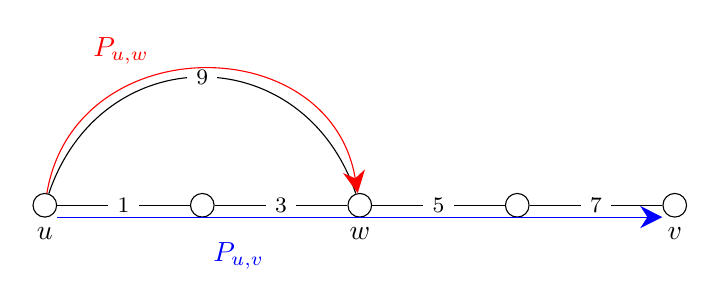
\begin{tikzpicture}[xscale=2]
	%%%S_uv
	\node[vert,label=below:$u$] (v1) at (1,0) {};
	\node[vert] (v2) at (2,0) {};
	\node[vert,label=below:$w$] (v3) at (3,0) {};
	\node[vert] (v4) at (4,0) {};
	\node[vert,label=below:$v$] (v5) at (5,0) {};
	\draw (v1) -- node[timelabel] {$1$} (v2) -- node[timelabel] {$3$}  (v3) -- node[timelabel] {$5$} (v4) -- node[timelabel] {$7$} (v5);
	\draw (v1) to [out=80,in=100,distance=2cm] node[timelabel] {$9$} (v3);
	
	\draw[transform canvas={yshift=-1.5mm}, blue]
	(v1) edge[diredge2]  node[pos=0.3,yshift=-2,label=below:$P_{u,v}$] {} (v5) ;
	
	\draw[red]
	(v1) edge[diredge2] [out=85,in=95,distance=2.1cm] node[pos=0.3,yshift=2,label=above:$P_{u,w}$] {} (v3) ;
\end{tikzpicture}
	\caption{An example of a temporal graph, where the fastest temporal path $P_{u,v}$ (in blue) from $u$ to $v$ is of duration $7$,
		while the fastest temporal path $P_{u,w}$ (in red) from $u$ to a vertex $w$ that is on a path $P_{u,v}$ is of duration $1$ and is not a subpath of $P_{u,v}$.		
		\label{fig:ftpExample}}
	\end{figure}

%\section{Results}

\section{\deltaExact}

In this section we study the hardness of \deltaExact. We first start with defining certain notions, that will be of use when solving the problem.

    \begin{definition}[Travel delays]
    Let $(G, \lambda, \Delta)$ be a temporal graph satisfying conditions of problem \deltaExact.
    Let $e_1=uv$ and $e_2=vz$ be two incident edges in $G$ with $e_1 \cap e_2 = v$.
    We define the \emph{travel delay} from $u$ to $z$ at vertex $v$, denoted with $\tau_v^{uz}$,
    as the difference of the labels of $e_2$ and $e_1$, where we subtract the value of the label of $e_1$ from the label of $e_2$,  modulo~$\Delta$.
    More specifically:
    \begin{equation}\label{eq:def-VertexWaitingTime}
       \tau_v^{uz} \equiv \lambda (e_2) - \lambda(e_1) \pmod \Delta.
    \end{equation}
    Similarly, $\tau_v^{zu} \equiv \lambda (e_1) - \lambda(e_2) \pmod \Delta$.
    \end{definition}
    Intuitively, the value of $\tau_v^{uz}$ represents how long a temporal path waits at vertex $v$ when first taking edge $e_1=uv$ and then edge $e_2 = vz$.

    From the above definition and the definition of the duration of the temporal path $P$ we get the following two observations.
    \begin{observation}\label{obs:durationPwithWaitingTimes}
        Let $P = (v_0, v_1, \dots, v_p)$ be the temporal path from $v_0$ to $v_p$.
        Then $d(P) = \sum_{i = 1}^{p-1} \tau_{v_i}^{v_{i-1}v_i} + 1 $.
    \end{observation}
    \begin{proof}
        For the simplicity of the proof denote $t_i = \lambda(v_{i-1}v_i)$, and suppose that $t_i \leq t_{i+1}$, for all $i \in \{1,2,3,\dots,p\}$.
        Then
        \begin{align*}
        \sum_{i = 1}^{p-1} \tau_{v_i}^{v_{i-1}v_i} + 1  
        &= \sum _{i = 1}^{p-1} (t_{i+1} - t_i) + 1 \\
        & = (t_2 - t_1) + (t_3  t_2) + \cdots + (t_p - t_{p-1}) + 1  \\
        & = t_{p-1} - t_1 + 1\\
        & = d(P)
        \end{align*}
        Now in the case when $t_i > t_{i+1}$ we get that $\tau_{v_i}^{v_{i-1}v_{i+1}} = \Delta + t_{i+1} - t_i$.
        At the end this still results in the correct duration as the last time we traverse the path $P$ is not exactly $t_p$ but $k \lambda + t_p$, for some $k$.
    \end{proof}
    We also get the following.
    \begin{observation}\label{obs:travel-delays-both-directions}
    Let $(G, \lambda, \Delta)$ be a temporal graph satisfying conditions of problem \deltaExact.
    For any two incident edges $e_1 = uv$ and $e_2 = vz$ on vertices $u,v,z \in V$, with $e_1 \cap e_2 = v$, we have $\tau_v^{zu} = \Delta - \tau_v^{uz} \pmod \Delta$.
    \end{observation}
    
    \begin{proof}
        Let $e_1 = uv$ and $e_2 = vz$ be two edges in $G$ for which $e_1 \cap e_2 = v$. 
        By the definition $\tau_v^{uz} \equiv \lambda (e_2) - \lambda(e_1) \pmod \Delta$ and $\tau_v^{zu} \equiv \lambda (e_1) - \lambda(e_2) \pmod \Delta$.
        Summing now both equations we get $\tau_v^{uz} + \tau_v^{zu} \equiv \lambda(e_2) - \lambda(e_1) + \lambda (e_1) - \lambda(e_2) \pmod \Delta$, and therefore $\tau_v^{uz} + \tau_v^{zu} \equiv 0 \pmod \Delta$, which is equivalent as saying $\tau_v^{uz} \equiv - \tau_v^{zu} \pmod \Delta$ or $\tau_v^{zu} = \Delta - \tau_v^{uz} \pmod \Delta$.
    \end{proof}

\begin{lemma} \label{lemma:unique-fastest-path-allDelays}
    Let $(G, \lambda, \Delta)$ be a temporal graph satisfying conditions of problem \deltaExact,
    and let $P=P_{1,k}$ be a fastest temporal path from $u=v_1$ to $v=v_k$ on $k$ vertices $v_1,v_2,\dots,v_k$.
    Let us denote with $P_{1,i}$ the sub-path of temporal path $P_{1,k}$, that starts at $v_1$ and finishes at $v_i$.
    Suppose that $P_{1,i}$ is also the fastest temporal path from $u=v_1$ to any other vertex $v_i$ in $P$.
    Then we can determine travel delays on $P$ using the following equation
    \begin{equation}\label{eq:trav-delays-paths}
        \tau_{v_i}^{v_{i-1},v_{i+1}} = D_{1,i+1} - D_{1,i},
    \end{equation}
    for all $i \in \{2,3, \dots, k-1\}$.
\end{lemma}

\begin{proof}
    Let $P$ be a fastest temporal path from $v_1$ to $v_k$ with the properties from the claim, and let $v_i$ be an arbitrary vertex in $P \setminus \{v_1,v_k\}$.
    Using the properties of fastest paths and the definition of duration, we can rewrite \cref{eq:trav-delays-paths} as follows
    \begin{align*}
        \tau_{v_i}^{v_{i-1},v_{i+1}} & = D_{1,i+1} - D_{1,i} =  d(P_{1,i+1}) - d(P_{1,i}) \\
        & \equiv 
        \left(\lambda(v_{i}v_{i+1}) - \lambda(v_1v_2) + 1\right) -  
        \left(\lambda(v_{i-1}v_{i}) - \lambda(v_1v_2) + 1\right) \pmod \Delta \\
        & \equiv \lambda(v_{i}v_{i+1}) - \lambda(v_{i-1}v_{i}) \pmod \Delta,
        \end{align*}
    which is exactly the definition of $\tau_{v_i}^{v_{i-1},v_{i+1}}$.
\end{proof}

\subsection{ \deltaExact\ is polynomial-time solvable on trees and paths}

Let $D$ be a matrix from \deltaExact, when the underlying graph $G$ of $D$ is a tree on $n$ vertices $\{v_1, v_2, \dots, v_n\}$.
Let $v_i,v_j$ be two arbitrary vertices in $G$. Then we know that there exists a unique (static) path $P$ among them.
Consequently, it follows that the temporal paths $P_{i,j}$ from $v_i$ to $v_j$ and $P_{j,i}$ from $v_j$ to $v_i$ are also unique, up to modulo of the period $\Delta$ of the labeling $\lambda$,
and therefore are the fastest.
Then $D$ is of the following form:
\begin{equation*}
    D_{i,j} =
    \begin{cases}
    0 & \text{if $i = j$}, \\
    1 & \text{if $v_i$ and $v_j$ are neighbours in G}\\
    d(P_{i,j}) & \text{else}
    \end{cases},
\end{equation*}
where $d(P_{i,j})$ is the duration of the (unique) temporal path $P_{i,j}$ from $v_i$ to $v_j$.

\begin{observation}\label{obs:travel-delays-in-trees}
    Let $v_i,v_j$  be arbitrary two vertices in a tree $G$. 
    Since there is a unique temporal path $P_{i,j}$ from $v_i$ to $v_j$, it is also the fastest one, therefore $d(P_{i,j}) = D_{i,j}$. 
    Note, all other vertices $v' \in P_{i,j} \setminus \{v_i,v_j\}$ are reached form $v_i$ using a part of the path $P_{i,j}$.
    Now using \cref{lemma:unique-fastest-path-allDelays}, we can determine the waiting times for all \emph{inner} vertices of the path $P_{i,j}$.
\end{observation}

\begin{theorem} \label{thm:deltaExact-PolyTimeTrees}
    \deltaExact\ can be solved in polynomial time on trees.
\end{theorem}

\begin{proof}
    Let $D$ be an input matrix for problem \deltaExact\ of dimension $n \times n$.
    Let us fix the vertices of the corresponding graph $G$ of $D$ as $v_1, v_2, \dots, v_n$, where vertex $v_i$ corresponds to the row and column $i$ of matrix $D$.
    This can be done in polynomial time as we need to loop through the matrix $D$ once and connect vertices $v_i, v_j$ for which $D_{i,j} = 1$. At the same time we also check if $D_{i,i} = 0$, for all $i \in [n]$.
    When $G$ is constructed we run DFS algorithm on it and check if it has no cycles.
    If at any step we encounter a problem, our algorithm stops and returns a negative answer.
    
    From now on we can assume that we know that the underlying graph $G$ of $D$ is a tree and we know how it looks like.
    For the next part of the algorithm we use \cref{obs:travel-delays-in-trees}.
    
    We pick an arbitrary vertex $v_i \in V(G)$ and check which vertex $v_j \in V(G)$ is furthest away from it, \ie we find a maximum element in the $i$-th row of the matrix $D$.
    We now take the unique path $P_{i,j}$ in $G$, which has to also be the fastest temporal path from $v_i$ to $v_j$, and using \cref{obs:travel-delays-in-trees} calculate waiting times at all inner vertices.
    We save those values in a matrix $T$, of size $n \times n \times n$, and mark vertices of the path  $P_{i,j}$ as visited.
    Matrix $T$ stores at the position $(k,j,\ell)$ the value corresponding to the travel delay at vertex $v_k$ when traveling from $v_{j}$ to $v_{\ell}$, \ie it stores the value $\tau_{v_k}^{v_{j}, v_\ell}$, where $v_j,v_\ell \in N(v_k)$. All other values of $T$ are set to \textsc{Null}.
    Now we repeat procedure, from vertex $v_i$, for vertices that are not marked as visited yet, \ie vertices in $V \setminus P_{i,j}$.
    We find a vertex in $V \setminus P_{i,j}$ that is furthest away from $v_i$ and repeat the procedure.
    When we have exhausted the $i$-th row of $D$,
    \ie vertex $v_i$ now reaches every vertex of $G$,
    we continue and repeat the procedure for all other vertices.
    If at any point we get two different values for the same travel delay at a specific vertex, then we stop with the algorithm and return the negative answer.
    If the above procedure finishes successfully we get the matrix $T$ with travel delays for all vertices in $G$, of degree at least $2$.
    The above calculation is performed in polynomial time, as for every vertex $v_i$ we inspect the whole graph once.
    \begin{lemma}\label{lemma:matrixT-travelDelays-tree}
        Matrix $T$ consists of travel delays of all vertices of degree at least $2$ in $G$.
    \end{lemma}
    \begin{proof}[Proof of \cref{lemma:matrixT-travelDelays-tree}]
        Note, by the definition of travel delays, a vertex of degree $1$ cannot have a travel delay.
        Suppose now that there is a vertex $v_i \in V(G)$ of degree at least $2$, for which our algorithm did not calculate its travel delay.
        Let $v_a, v_b$ be two arbitrary neighbors of $v_i$, \ie $v_a v_i, v_i v_b \in E(G)$.
        Since $G$ is a tree, the unique (and fastest) temporal path from $v_a$ to $v_b$ passes through $v_i$.
        When our algorithm was inspecting the row of $D$ corresponding to vertex $v_a$, it had to consider the temporal path from $v_a$ to $v_b$. 
        At this point, it calculated $\tau_{v_i}^{v_a,v_b}$. 
        Since this is true for any two $v_a, v_b \in N(v_i)$, it cannot happen that some travel delay at $v_i$ is not calculated.
        Since $v_i$ was an arbitrary vertex in $G$ of degree at least $2$, the claim holds.
    \end{proof}
    
    Now, given the matrix of travel delays $T$, we can find a labeling $\lambda$ that satisfies $D$.
    We start by fixing a label of one arbitrary edge as $a$, where $a \in [\Delta]$.
    Knowing the label of one edge, and all waiting times in $T$, we can uniquely determine the labels of all other edges.
    More specifically, if we know that $\lambda(v_i v_j) = a$, then for all $v_k \in N(v_i)$ (resp.~$v_{k'} \in N(v_j)$)
    the value $\lambda(v_iv_k) \equiv a + \tau_{v_i}^{v_j,v_k} \pmod \Delta $ (resp.~$\lambda(v_j v_{k'}) \equiv a + \tau_{v_j}^{v_i,v_{k'}} \pmod \Delta $).
    Since there are $\Delta$ options to fix the first label, we can find $\Delta$ different labelings satisfying $D$.
    Note, w.l.o.g. we can start determining the labeling $\lambda$ by setting $\lambda(v_1v_2) = 1$.
    It is not hard to see, that also the calculation of the labeling $\lambda$ takes polynomial time, as we have to traverse the graph exactly once, to successfully fix the labeling. Therefore, all together the whole algorithm is performed in polynomial time.
\end{proof}

\subsection{ \deltaExact\
is polynomial-time solvable on cycles}

Let us observe some properties of the matrix $D$ from \deltaExact, when the underlying graph $G$ of $D$ is a cycle $C_n = \{v_1, v_2, \dots, v_n\}$  on $n$ vertices.
By the definition, each vertex is on distance $0$ from itself. This corresponds with all diagonal entries of $D$ being $0$.
Now, let us observe that each vertex $v_i$ has exactly two neighbours in $C_n$, namely $v_{i-1}$ and $v_{i+1}$,
therefore for all $i\in [n]$ we set $D_{i,i-1} = D_{i, i+1} = 1$, where indices are taken modulo $n$.
This results in the upper and lower diagonal of $D$ having all $1$'s, together with $D_{1,n} = D_{n,1} = 1$.
The matrix $D$ is of the following form
\begin{equation} \label{eq:D-matrixForCycles}
  D = 
  \begin{bmatrix}
    0 & 1 &  &  &  & 1\\
    1 & 0 & 1 &  &  & \\
    & 1 & 0 & 1 & & \\
    & & \ddots & \ddots & \ddots &   \\
    &   & &1 &  0 & 1\\ 
    1 &  &  &  &1 &  0 
  \end{bmatrix},
\end{equation}
where the empty entries consists of positive integers different than $1$.

Given a matrix in the input of \deltaExact\ we can check in $O(n^2)$ time if it is of correct form, by traversing it once. If it is not of correct form, our algorithm stops and returns the negative answer.
From now on, we assume, that the input matrix has the same form as $D$ from \cref{eq:D-matrixForCycles}.

Let $v_i$ be an arbitrary vertex in the cycle $C_n =\{v_1, v_2, \dots, v_n\}$.
Vertex $v_i$ can reach an arbitrary vertex $v_k \in C_n$ using a positive side of the cycle (\ie going from $v_i$ to $v_{i+1},  v_{i+2}$, etc.), 
and using the negative side of the cycle (\ie going from $v_i$ to $v_{i-1}, v_{i-2}$, etc.).
Let us denote with the $d^+(i,k)$ the duration of the temporal path from $v_i$ to $v_k$ using the positive side of the cycle,
and with $d^-(i,k)$, the duration of the temporal path from $v_i$ to $v_k$ using the negative side of the cycle.
Since these two are the only possible paths from $v_i$ to $v_k$ in $C_n$ we know that $D_{i,k} = min \{d^+(i,k), d^-(i,k)\}$.

\begin{lemma} \label{lemma:poly-delta-cycle-monotonicity}
    If vertex $v_i$ reaches vertex $v_j$ the fastest, using the positive (resp.~negative) side of the cycle, \ie $v_i, v_{i+1}, \dots, v_{j-1}, v_j$ (resp. $v_i, v_{i-1}, \dots, v_{j+1}, v_j$),
    then $v_i$ reaches all other vertices $v_k$, where $k \in \{i+1, i+2, \dots, j-1\}$ (resp.~ $k \in \{i-1, i-2, \dots, j+1\}$)
    using the same, positive (resp.~negative) side of the cycle,
    where the indices are taken modulo $n$.
\end{lemma}
\begin{proof}
    Let $v_i, v_j$ be two arbitrary vertices in $C_n$ and suppose that $D_{i,j} = d^+(i,j)$,
    but there exists a vertex $v_k$ from $C_n$, where $k \in \{i+1, i+2, \dots, j-1\}$,
    for which $D_{i,k} \neq d^+(i,k)$.
    Then $d^-(i,k)$ passes through vertex $v_j$, and we can split the path from $v_i$ to $v_k$ into two pieces, 
    first from $v_i$ to $v_j$ and the second one from $v_k$ to $v_j$.
    So 
    \begin{equation} \label{eq:poly-delta-cycle-monotonicity}
        d^-(i,k) = d^-(i,j) + d^-(j,k)^*,
    \end{equation} where $d^-(j,k)^*$ is the duration of the path from $v_j$ to $v_k$, using the negative side of the cycle, with consideration that we come to vertex $v_j$ at time $d^-(i,j)$ and we potentially have to wait there for some positive amount of time, before we continue to $v_j$
    (\ie $d^-(j,k)^* \geq d^-(i,j) \geq D_{j,k}$ includes some waiting time at vertex $v_j$).
    By the assumption we know that $d^+(i,j) \leq d^-(i,j)$, so we can rewrite \cref{eq:poly-delta-cycle-monotonicity} as
    $d^-(i,k) \leq d^+(i,j) + d^-(j,k)^*$. This means that we can reach $v_k$ from $v_j$ by going from $v_i$ to $v_j$ using the positive side of the cycle, wait some time at $v_j$, before we continue back to $v_j$.
    In the above construction vertex $v_k$ is visited twice. By the definition, the fastest temporal path from $v_i$ to $v_k$ visits $v_k$ exactly once. Therefore we can stop at $v_k$ already when traveling from $v_i$ to $v_j$ the first time, using the positive side of the cycle.
    It follows that $D_{i,j} = d^+(i,j) \leq d^-(i,j)$, which contradicts with our assumption.
\end{proof}

Let $v_i$ and $v_j$ be two arbitrary vertices in the cycle $C_n$, for which $v_i v_j \notin E(C_n)$.
Suppose that $P^+_{i,j}$ (resp.~$P^-_{i,j})$ is the fastest temporal path from $v_i$ to $v_j$, using the positive (resp.~negative) side of the cycle, 
\ie $v_i, v_{i+1}, \dots, v_{j-1}, v_j$ (resp. $v_i, v_{i-1}, \dots, v_{j+1}, v_j$).
Then by \cref{lemma:poly-delta-cycle-monotonicity} and \cref{lemma:unique-fastest-path-allDelays},
we get that we can determine all travel delays at vertices of $P^+_{i,j} \setminus \{v_i, v_j\}$ (resp.~$P^-_{i,j} \setminus \{v_i, v_j\}$).


Let $v_i$ be an arbitrary vertex of $C_n$. Let us look at the row $i$ of the matrix $D$, which corresponds to the durations of fastest temporal paths from $v_i$ to all other vertices $v_j \in C_n$.
Using \cref{lemma:poly-delta-cycle-monotonicity} we know that $v_i$ will reach some consecutive vertices $v_{i+1}, v_{i+2}, \dots, v_j$ the fastest, using the positive side of the cycle 
and $v_{i-1}, v_{i-2}, \dots, v_{j+1}$ the fastest, using the negative side of the cycle.
Suppose $v_j \in C_n$ is the last vertex $v_i$ reaches using the positive side of the cycle, and $v_{j+1}$ the last vertex that is reached using the negative side of the cycle.
Then we know that $D_{i,i+1} < D_{i,i+2} < \cdots< D_{i,j-1} < D_{i,j}$ and 
$D_{i,i-1} < D_{i,i-2} < \cdots < D_{i,j+2} < D_{i,j+1}$.
Note that it can happen that $v_j = v_{j+1}$, \ie to reach vertex $v_j$ from $v_i$ the fastest, we can use either positive or negative side of the cycle.
Using the above observations, every row $i$ ($i \in [n]$) of matrix $D$ has two (or one) maximum elements, one at position $j$ and the other at position $j+1$, where $j, j+1 \in [n]$ and the indices are considered modulo $n$.
Let us denote these two values as $m_i^1$ and $m_i^2$.
The row $i$ of $D$ is of the following form, it has a $0$ at the entry $i$, it has $1$ at entries $i-1, i+1$,
the values increase on the positions $i+1, i+2, i+3, \dots, j-1, j$ for some $j$ with value $m_i^1$, 
and on the other side, values increase on the positions $i-1, i-2, i-3, \dots, j+2, j+1$ for some $j+1$ with value $m_i^2$,
where indices are taken modulo $n$.

Knowing this, we can split the vertices $v_j \in V(C_n) \setminus \{v_i\}$ into two parts, ones that are reached from $v_i$ the fastest using the positive side of the cycle and ones that are reached using the negative side of the cycle.
To determine these two sets we do the following.
We fix a vertex $v_i \in C_n$ and check its corresponding row in the matrix $D$. 
We determine two max values $m_i^1$ and $m_i^2$ at positions $j$ and $j+1$ (modulo $n$), respectively,
for which it has to hold that
$D_{i,i+1} < D_{i,i+2} < \cdots< D_{i,j-1} < D_{i,j}=m_i^1$ and 
$D_{i,i-1} < D_{i,i-2} < \cdots < D_{i,j+2} < D_{i,j+1}=m_i^2$.
Note, it can also happen that $m_i^1 = m_i^2$. 
Now denote the path that uses the positive side of the cycle, from $v_i$ to $v_j$, as $P^+_i$ and
the path that uses the negative side of the cycle, from $v_i$ to $v_{j+1}$, as $P^-_i$.
By \cref{lemma:poly-delta-cycle-monotonicity} and \cref{lemma:unique-fastest-path-allDelays} we can calculate travel delays at every vertex $v_k \in C_n \setminus \{v_i, v_j, v_{j+1}\}$,
which we store in a list $T$ of length $n$,
where the entry at the position $k$ corresponds to the travel delay at vertex $v_k$ when traveling from $v_{k-1}$ to $v_{k+1}$.
Note, from \cref{obs:travel-delays-both-directions} it follows, that it is enough to store the value of the travel delay in one direction (\ie knowing $\tau_v^{u,w}$ we know also $\tau_v^{w,u}$).
We repeat the above procedure for all rows in the matrix $D$, \ie for all vertices $v_i \in C_n$.
Calculation in one row is performed in $O(n)$ time, repeating it for all rows we need $O(n^2)$ time.

To determine the labeling $\lambda$ satisfying the matrix $D$, we have to make sure that we have calculated travel delays for all vertices.

\begin{lemma}
List $T$ of travel delays has non-empty values at all positions, \ie we have successfully calculated travel delays for all vertices.
\end{lemma}
\begin{proof}
    Throughout the proof we
    denote with $d^+(i,j)$ the duration of the temporal path that starts at $v_i$ and finishes at $v_j$, that uses the positive side of the cycle $C_n$,
    and similarly with $d^-(i,j)$ the duration of the temporal path that starts at $v_i$ and finishes at $v_j$, that uses the negative side of the cycle $C_n$,
    where indices are taken modulo $n$.
    
    Suppose for the contradiction that the statement of the claim does not hold. Then there exists a vertex $v_i \in C_n$, for which we did not calculate its travel delay.
    Let $v_j \in C_n \setminus \{v_i\}$ be an arbitrary vertex. 
    Note that the only time we cannot calculate the travel delay at vertex $v_i$, when considering vertex $v_j$, is in this case when $v_i$ is one of the maximum elements in $D_j$, \ie $v_i$ is a vertex that is on a maximum duration from $v_j$.
    This has to hold for all vertices $v_j$, therefore $v_i$ has to be on the maximum distance from every vertex $v_j \in C_n \setminus \{v_i\}$.
    It then also has to hold for vertices $v_{i-1}, v_{i+1}$, that are neighbours of $v_i$.
    We know that in this case $d^+(i-1,i) = 1, d^-(i+1,i) = 1$.
    Since $v_i$ has to be on the maximum duration from both of them 
    (\ie is one of the two maximum values $m^1_{i-1}, m^2_{i-1}$ for vertex $v_{i-1}$ and one of the two maximum values $m^1_{i+1}, m^2_{i+1}$ for vertex $v_{i+1}$),
    we know that 
    \begin{align}\label{eq:cycle-travel-delays-all}
        & d^+(i+1,i-1) < d^-(i+1,i-1) & \text{and}\\
        & d^-(i-1,i+1) < d^+(i-1,i+1).
    \end{align}
    If this would not hold, the fastest path would go through $v_i$ and we would be able to calculate the travel delay at $v_i$.
    
    Denote the labels $\lambda(v_{i-1}v_i) = a, \lambda(v_{i}v_{i+1})=a'$, and $\lambda(v_{i-2}v_{i-1} = b, \lambda (v_{i+1}v_{i+2})=b'$, where $a,a',b,b' \in [\Delta]$.
    W.l.o.g. we can suppose that $a \geq a'$.
    Therefore, using the definition for the duration of temporal paths, we get that
    $d^+(i+1,i-1) = (k \delta + b) - b' + 1$, where $k$ is some non-negative integer, and $d^-(i+1,i-1) = a - a' + 1$.
    Using the first inequality from \cref{eq:cycle-travel-delays-all} we get that 
    $(k \delta + b) - b' +1 < a - a' + 1$ which is equivalent to $(k \delta + b) - b' < a - a'$, which can be true only when $k = 0$, but because the duration is positive we get that $b > b'$ and
    $b - b' < a - a'$.
    Now again using the definition of the duration, we get
    $d^+(i-1,i+1)= (k\delta + a') - a + 1$, where $k$ is some non-negative integer, but since $v_{i-1}v_i$ and $v_iv_{i+1}$ are incident edges, we know also that $k=1$, therefore $d^+(i-1,i+1)= \delta + a - a + 1$. 
    Again by the definition, $d^-(i-1,i+1) = (k' \delta + b') -b + 1$, for some non-negative integer $k'$.
    Using the second inequality from \cref{eq:cycle-travel-delays-all} we get that 
    $(k' \delta + b') -b + 1 < \delta + a - a + 1$.
    Which is equivalent to  $(k' \delta + b') -b < \delta + a' - a $. This can hold only when $k' = 1$, in that case we get $ \delta + b' -b < \delta + a' - a $ which is equivalent to $b' -b < a' - a$.
    This is in the contradiction with the inequality  $b - b' < a - a'$ as this is equivalent to $b'-b > a'-a$.
    
    Therefore it cannot happen that there is a vertex $v_i$ for which we cannot calculate its travel delay in $C_n$.
\end{proof}

All of the above observations imply the following result.
\begin{theorem}
    \deltaExact\ can be solved in polynomial time on cycles.
\end{theorem}

\begin{proof}
As stated above, we can determine travel delays at every vertex in $O(n^2)$ time. 
Once all of the delays are calculated, we have to only construct the labeling $\lambda$ that satisfies the matrix $D$. 
We start by fixing a label of one edge as $a$, where $a \in [\Delta]$.
Knowing the label of edge $v_1v_2$ and all waiting times in $T$, we can uniquely determine the labels of all other edges.
More specifically, if we know that $\lambda(v_i v_j) = a$, then for all $v_k \in N(v_i)$ (resp.~$v_{k'} \in N(v_j)$)
the value $\lambda(v_iv_k) \equiv a + \tau_{v_i}^{v_j,v_k} \pmod \Delta $ (resp.~$\lambda(v_j v_{k'}) \equiv a + \tau_{v_j}^{v_i,v_{k'}} \pmod \Delta $).
Since there are $\Delta$ options to fix the first label, we can find $\Delta$ different labelings satisfying $D$.
Note, w.l.o.g. we can start determining the labeling $\lambda$ by setting $\lambda(v_1v_2) = 1$.
\end{proof}

    
\section{\deltaExact\ is NP-hard}

\begin{theorem}
	\deltaExactLong\ is \NP-hard.
\end{theorem}

\begin{proof}
	We present a polynomial-time reduction from the NP-hard problem NAE 3-SAT~\cite{Schaefer1978complexity}. Here we are given a formula $\phi$ in conjunctive normal form, where each clause contains exactly 3 literals (with three distinct variables).
    A NAE clause evaluates to \textsc{True} iff not all of its literals are equal.
    We construct an instance $D^\phi$ of \deltaExact\ as follows.

 We start by describing the vertex set of the underlying graph $G$ of  $D^\phi$.
\begin{itemize}
\item For each variable $x_i$ in $\phi$, we create three variable vertices $x_i, x_i^T, x_i^F$.
\item For each clause $c$ in $\phi$, we create one clause vertex $c$.
\item We add one additional super vertex $v$.
\end{itemize}
Next, we describe the edge set of $G$.
\begin{itemize}
\item For each variable $x_i$ in $\phi$ we add the following five edges: 
$x_i x_i^T, x_i x_i^F, x_i^T x_i^F, x_i^T v$ and $ x_i^Fv$.
\item For each pair of variables $x_i,x_j$ in $\phi$ with $i \neq j$ we add the following four edges: 
$x_i^T x_j^T, x_i^Tx_j^F, x_i^Fx_j^T$ and $x_i^Fx_j^F$.
\item For each clause $c$ in $\phi$ we add one edge for each literal. Let $x_i$ appear in $c$. If $x_i$ appears non-negated in $c$ we add edge $c x_i^T$. 
If $x_i$ appears negated in $c$ we add edge $c x_i^F$.
\end{itemize}
This finishes the construction of $G$.
For an example see~\cref{fig:NP-example}.

%
\begin{figure}[htb]
	\noindent
	\makebox[\textwidth]{
		\centering
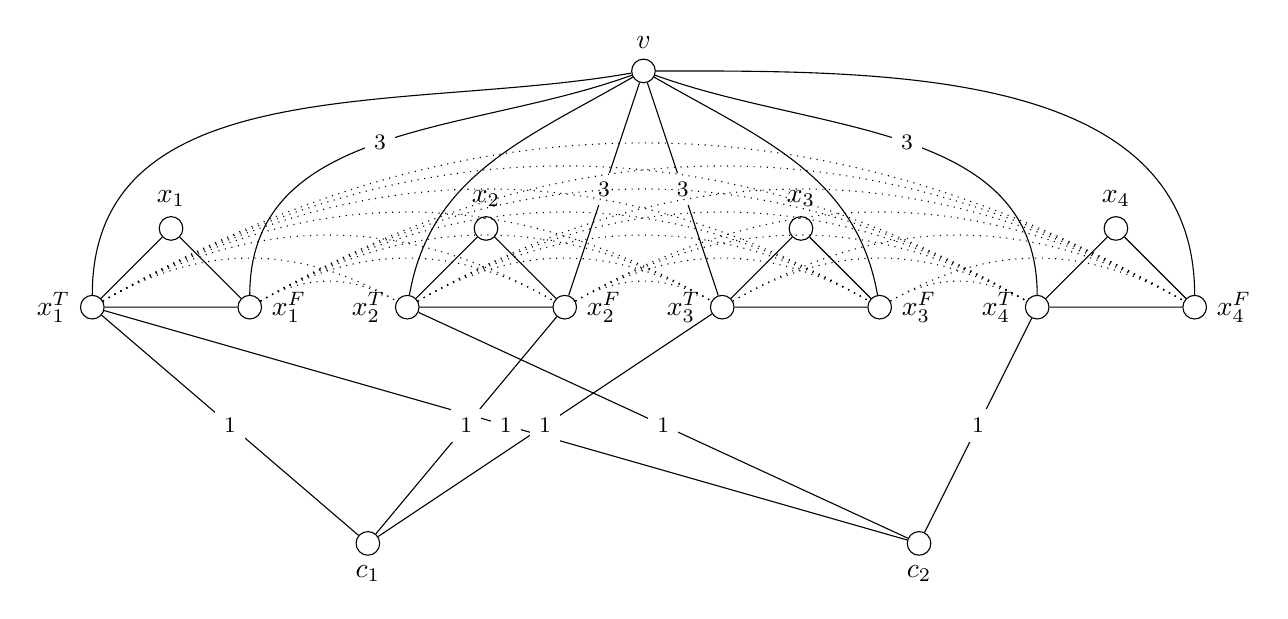
\begin{tikzpicture}%[xscale=2]

	%%Variable X1
	\node[vert,label=left:$x_1^T$] (x1t) at (1,0) {};
	\node[vert,label=right:$x_1^F$] (x1f) at (3,0) {};
	\node[vert,label=above:$x_1$] (x1) at (2,1) {};
	\draw (x1t) -- (x1f) -- (x1) -- (x1t);
	
	%%Variable X2
	\node[vert,label=left:$x_2^T$] (x2t) at (5,0) {};
	\node[vert,label=right:$x_2^F$] (x2f) at (7,0) {};
	\node[vert,label=above:$x_2$] (x2) at (6,1) {};
	\draw (x2t) -- (x2f) -- (x2) -- (x2t);
	
	%%Variable x3
	\node[vert,label=left:$x_3^T$] (x3t) at (9,0) {};
	\node[vert,label=right:$x_3^F$] (x3f) at (11,0) {};
	\node[vert,label=above:$x_3$] (x3) at (10,1) {};
	\draw (x3t) -- (x3f) -- (x3) -- (x3t);
	
	%%Variable x4
	\node[vert,label=left:$x_4^T$] (x4t) at (13,0) {};
	\node[vert,label=right:$x_4^F$] (x4f) at (15,0) {};
	\node[vert,label=above:$x_4$] (x4) at (14,1) {};
	\draw (x4t) -- (x4f) -- (x4) -- (x4t);
	
	%%vertices for clauses c1, c2 + vertex v
	\node[vert,label=above:$v$] (v) at (8,3) {};
	\node[vert,label=below:$c_1$] (c1) at (4.5,-3) {};
	\node[vert,label=below:$c_2$] (c2) at (11.5,-3) {};
	
	%%% edges between x1 gadget and v,c1,c2
	\draw (x1t) to node[timelabel] {$1$} (c1);
	\draw (x1t) to node[timelabel] {$1$} (c2);
	\draw (x1t) to [out=90,in=190] (v);
	\draw (x1f) to [out=90,in=200] node[timelabel] {$3$} (v);
	
	%%% edges between x2 gadget and v,c1,c2
	\draw (x2f) to node[timelabel] {$1$} (c1);
	\draw (x2t) to node[timelabel] {$1$} (c2);
	\draw (x2t) to [out=80,in=210]  (v);
	\draw (x2f) to node[timelabel] {$3$} (v);
	
	%%% edges between x3 gadget and v,c1
	\draw (x3t) to node[timelabel] {$1$} (c1);
	\draw (x3t) to node[timelabel] {$3$} (v);
	\draw (x3f) to [out=100,in=330] (v);
	
	%%% edges between x4 gadget and v,c2
	\draw (x4t) to node[timelabel] {$1$} (c2);
	\draw (x4t) to [out=90,in=340] node[timelabel] {$3$} (v);
	\draw (x4f) to [out=90,in=360] (v);
	
	%% edges among xt, xf vertices
	%x1 to all
	\draw [dotted] (x1t) [out=30,in=150] to (x2t);
	\draw [dotted] (x1t) [out=30,in=150] to (x3t);
	\draw [dotted] (x1t) [out=30,in=150] to (x4t);
	\draw [dotted] (x1t) [out=30,in=150] to (x2f);
	\draw [dotted] (x1t) [out=30,in=150] to (x3f);
	\draw [dotted] (x1t) [out=30,in=150] to (x4f);
	
	\draw [dotted] (x1f) [out=30,in=150] to (x2t);
	\draw [dotted] (x1f) [out=30,in=150] to (x3t);
	\draw [dotted] (x1f) [out=30,in=150] to (x4t);
	\draw [dotted] (x1f) [out=30,in=150] to (x2f);
	\draw [dotted] (x1f) [out=30,in=150] to (x3f);
	\draw [dotted] (x1f) [out=30,in=150] to (x4f);
	%x2 to all
	\draw [dotted] (x2t) [out=30,in=150] to (x3t);
	\draw [dotted] (x2t) [out=30,in=150] to (x4t);
	\draw [dotted] (x2t) [out=30,in=150] to (x3f);
	\draw [dotted] (x2t) [out=30,in=150] to (x4f);
	
	\draw [dotted] (x2f) [out=30,in=150] to (x3t);
	\draw [dotted] (x2f) [out=30,in=150] to (x4t);
	\draw [dotted] (x2f) [out=30,in=150] to (x3f);
	\draw [dotted] (x2f) [out=30,in=150] to (x4f);
	%x3 to all
	\draw [dotted] (x3t) [out=30,in=150] to (x4t);
	\draw [dotted] (x3t) [out=30,in=150] to (x4f);
	
	\draw [dotted] (x3f) [out=30,in=150] to (x4t);
	\draw [dotted] (x3f) [out=30,in=150] to (x4f);
\end{tikzpicture}
}
\caption{Example of the temporal graph $(G_\phi,\lambda)$ from the NP-hardness reduction, 
	where the 3-SAT formula $\phi$ is of form $\phi = (x_1 \vee \overline{x_2} \vee x_3) \wedge (\overline{x_1} \vee x_2 \vee x_4)$.
For the simplicity we draw edges between vertices $x_i^T$ and $x_j^F$ (where $i \neq j$) with a dotted line.
Presented is the labeling of $G_\phi$, corresponding to the assignment $x_1=x_2=\textsc{True}$ and $x_3,x_4=\textsc{False}$,
where all unlabeled edges get the label $2$.
\label{fig:NP-example}}
\end{figure}
%
Now we specify the distances in the matrix $D^\phi$ between all vertex pairs.
For the sake of simplicity we write $D^\phi _{u,v}$ as $d(u,v)$,
where $u,v$ are two vertices of $G$. 
We start by setting the value of $d(u,v) = 1$ where $u$ and $v$ are two adjacent vertices in $G$.
\begin{itemize}
    %\item For each variable $x$ in $\phi$ we specify the following distances between the non-adjacent variable vertices:
    %$d(x_1,x_2)=2$. 
    %\item For pair of variable $x,y$ in $\phi$ with $x\neq y$ we specify the following 
    %$d(x_1,y^T)=d(x_1,y^F)=3$, $d(x_2,y^T)=d(x_2,y^F)=2$.
    \item For each variable $x_i$ in $\phi$ and the super vertex $v$
    we specify the following distances:
    $d(x_i,v)=2$ and $d(v,x_i)= \Delta $. %, $d(x_2,v)=3$.
    \item For each clause $c$ in $\phi$ and the super vertex $v$
    we specify the following distances:
    $d(c,v)=2$ and $d(v,c)= \Delta - 1$.
    \item Let $x_i$ be a variable that appears in clause $c$, then  we specify the following distances:
    $d(c,x_i)=2$ and $d(x_i,c)=\Delta$.
    If $x_i$ appears non-negated in $c$ we specify the following distances:
    $d(c,x_i^F)=2$ and $d(x_i^F,c)=\Delta$.
    If $x_i$ appears negated in $c$ we specify the following distances:
    $d(c,x_i^T)=2$ and $d(x_i^T,c)=\Delta$.
    \item Let $x_i$ be a variable that does \emph{not} appear in clause $c$, then we specify the following distances:
    $d(x_i,c)=\Delta$, $d(c,x_i)=2\Delta + 2$
    and
    $d(c,x_i^T)=d(c,x_i^F)=2$, $d(x_i^T,c)=d(x_i^F,c)=\Delta$. 
    \item For each pair of variables $x_i \neq x_j$ in $\phi$ we specify the following distances:
    $d(x_i,x_j)=2\Delta +1$ and
    $d(x_i,x_j^T)=d(x_i,x_j^F)=\Delta + 1$.
    \item For each pair of clauses $c_i \neq c_j$ in $\phi$ we specify the following distances:
    $d(c_i,c_j)= \Delta + 1$.
\end{itemize}
This finishes the construction of an instance $D^\phi$ of \deltaExact\, which can clearly be done in polynomial time. In the remainder we show that $D^\phi$ is a yes-instance of \deltaExact\ if and only if NAE 3-SAT formula $\phi$ is satisfiable.

$(\Rightarrow)$: Assume the constructed instance $D^\phi$ of \deltaExact\ is a yes-instance. 
Then there exist a label $\lambda(e)$ for each edge $e\in E(G)$ such that for each vertex pair $u,w$ in the temporal graph $(G,\lambda)$ we have that a fastest temporal path from $u$ to $w$ is of duration $d(u,w)$. 
%In particular, for any two vertices $u,w$ with $d(u,w)=\infty$ we have that there does not exist a temporal path from $u$ to $w$ in $(G,\lambda)$.

We construct a satisfying assignment for $\phi$ as follows. For each variable $x_i$, 
if $\lambda(x_i x_i^T)=\lambda(x_i^T v)$, then we set $x_i$ to \textsc{True}, otherwise we set $x_i$ to \textsc{False}.

To show that this yields a satisfying assignment, we need to prove some properties of the labeling $\lambda$.
First, observe that adding an integer $t$ to all time labels does not change the duration of any temporal paths. 
Second, observe that if for two vertices $u,w$ we have that $d(u,w)$ equals the distance between $u$ and $w$ in $G$
(\ie the duration of the fastest temporal path from $u$ to $w$ equals the distance of the shortest path between $u$ and $w$), 
then there is a shortest path $P$ from $u$ to $w$ in $G$ such that 
the labeling $\lambda$ assigns consecutive time labels to the edges of $P$.


Let $\lambda(x_i x_i^T)=t$ and $\lambda(x_i x_i^F)=t'$, for an arbitrary variable $x_i$. 
If both $\lambda(x_i^T v)\neq t+1$ and $\lambda(x_i^F v)\neq t'+1$, then $d(x_i,v)>2$, which is a contradiction. 
Thus, for every variable $x_i$, we have that $\lambda(x_i^T v)= t+1$ or $\lambda(x_i^F v)= t'+1$ (or both). 
In particular, this means that if $\lambda(x_i x_i^F)=\lambda(x_i^F v)$, then we set $x_i$ to \textsc{False}, since in this case $\lambda(x_i x_i^T)\neq\lambda(x_i^T v)$.

%Furthermore, we have that if $x$ appears non-negated in clause $c$, then $\lambda(\{c,x^T\})=t-1$, otherwise we have $d(c,x^T)>2$. Symmetrically, we have that if $x$ appears negated in clause $c$, then $\lambda(\{c,x^F\})=t'-1$, otherwise we have $d(c,x^F)>2$.

Now assume for a contradiction that the described assignment is not satisfying. Then there exists a clause $c$ that is not satisfied. 
Suppose that $x_1, x_2, x_3$ are three variables that appear in $c$.
Recall that we require $d(c,v)=2$ and $d(v,c)=\Delta -1$. 
The fact that $d(c,v)=2$ implies that we must have a temporal path consisting of two edges from $c$ to $v$, 
such that the two edges have consecutive labels. 
By construction of $G$ there are three candidates for such a path, one for each literal of $c$. 
Assume w.l.o.g\ that $x_1$ appears in $c$ non-negated (the case of a negated appearance of $x_1$ is symmetrical) and that the temporal path realizing $d(c,v)=2$ goes through vertex $x_1^T$. 
Let us denote with $t = \lambda(x_1^T v)$.
It follows that $\lambda(x_1^T c)=\lambda(x_1^T v)-1 = t - 1$.
Furthermore, since $d(c,x_1)=2$ we also have that $\lambda(x_1^T c)=\lambda(x_1 x_1^T)-1$. 
Therefore $\lambda(x_1 x_1^T)=\lambda(x_1^T v) = t$. 
Which implies that $x_1$ is set to \textsc{True}.
%
Let us observe paths from $v$ to $c_1$.
We know that $d(v,c)=\Delta -1$.
The underlying path of the fastest temporal path from $v$ to $c$, that goes through $x_1^T$ is the path $P = (v,x_1^T,c)$.
Since $\lambda(x_1^Tc) > \lambda(x_1^T v)$ we get that the duration of the temporal path $(P,\lambda)$ is equal to 
$d(P,\lambda)= (\Delta + t-1) - t + 1 = \Delta$.
This implies that
the fastest temporal path from $v$ to $c$ is not $(P,\lambda)$ and therefore does not pass through $x_1^T$.
Since there are only two other vertices connected to $c$, 
we have only two other edges incident to $c$, that can be used on a fastest temporal path
$v$ to $c$.
Suppose now w.l.o.g\ that also $x_2$ appears in $c$ non-negated (the case of a negated appearance of $x_2$ is symmetrical) and that the temporal path realizing $d(v,c)=\Delta$ goes through vertex $x_2^T$.
Let us denote with $t' = \lambda(x_2^T v)$.
Since the fastest temporal path from $v$ to $c$ is of the duration $\delta - 1$,
and the edge $x_2^T c$ is the only edge incident to vertex $c$ and edge $ x_2^T v$,
it follows that $\lambda(x_2^T c) \geq \lambda(x_2^T v) - 2 = t' - 2$.
Since $d(x_2,v) = 2$ it follows that $\lambda(x_2 x_2^T) = \lambda (x_2^T v) - 1 = t' - 1$.
Knowing this and the fact that $d(x_2,c)=2$, we get that $\lambda(x_2^T c)$ must be equal to $t'-2$.
Therefore the fastest temporal path from $v$ to $c$ passes through edges $ x_2^Tv$ and $x_2^Tc$.
In the above we have also determined that $\lambda(x_2x_2^T) \neq \lambda ( x_2^Tv)$,
which implies that $x_2$ is set to \textsc{True}.
But now we have that $x_1,x_2$ both appear in $c$, where one of them is \textsc{True}, while the other is \textsc{False},
which implies that the clause $c$ is satisfied, a contradiction. 


%Assume w.l.o.g.\ that variable $x$ appears non-negated in clause $c$. Then we have that $\{c,x^T\}\in E(G)$. Assume that $\lambda(\{c,x^T\})=t$. Recall that we have specified $d(c,x_2)=2$. Hence we have that $\lambda(\{x_2,x^T\})=t+1$.

$(\Leftarrow)$: Assume that $\phi$ is satisfiable. Then there exists a satisfying assignment for the variables in $\phi$.

We construct a labeling $\lambda$ as follows.
\begin{itemize}
    \item All edges incident with a clause vertex $c$ obtain label one.
    %\item For each variable $x$, we set $\lambda(\{x^T,x^F\})=1$.
    \item If variable $x_i$ is set to \textsc{True}, we set $\lambda(x_i^F v)=3$.
    \item If variable $x_i$ is set to \textsc{False}, we set $\lambda(x_i^T v)=3$.
    \item We set the labels of all other edges to two.
\end{itemize}
For an example of the constructed temporal graph see~\cref{fig:NP-example}.
We now verify that all distances are realized.
\begin{itemize}
    \item For each variable $x_i$ in $\phi$ we have to check that $d(x_i,v)=2$
    and $d(v,x_i)=\Delta$. 
    
    If $x_i$ is set to \textsc{True}, then there is a temporal path from $x_i$ to $v$ via 
    $x_i^F$ of duration $2$, since
    $\lambda(x_i x_i^F)=2$ and $\lambda(x_i^F v)=3$.
    For a temporal path from $v$ to $x_i$ we observe the following.
    The only possible labels to leave the vertex $v$ are $2$ and $3$, which take us from $v$ to $x_j^T$ or $x_j^F$ of some variable $x_j$.
    The only two edges incident to $x_i$ have labels $2$, therefore the fastest path from $v$ to $x_i$
    cannot finish before the time $\Delta + 2$.
    The fastest way to leave $v$ and enter to $x_i$ would then be to leave $v$ at edge $x_i^Fv$ with label $3$,
    and continue to $x_i$ at time $\Delta + 2$,
    which gives us the desired duration $\Delta$.
    
    If $x_i$ is set to \textsc{False}, then, by similar arguing, 
    there is a temporal path from $x_i$ to $v$ via $x_i^T$ of duration $2$,
    and a temporal path from $v$ to $x_i$, through $x_i^F$ of duration $\Delta$.

    \item For each clause $c$ in $\phi$ we have to check that $d(c,v)=2$
    and $d(v,c)=\Delta - 1$:

    Suppose $x_i,x_j,x_k$ appear in $c$.
    Since we have a satisfying assignment at least one of the literals in $c$ is set to \textsc{True} and at least one to \textsc{False}. 
    Suppose $x_i$ is the variable of the literal that is \textsc{True} in $c$,
    and $x_j$ is the variable of the literal that is \textsc{False} in $c$.
    Let $x_i$ appear non-negated in $c$ and is therefore set to \textsc{True} (the case when $x_i$ appears negated in $c$ and is set to \textsc{False} is symmetric).
    Then there is a temporal path from $c$ to $v$ through $x_i^T$ such that $\lambda(x_i^T c)=1$ and $\lambda(x_i^T v)=2$. 
    Let $x_j$ appear non-negated in $c$ and is therefore set to \textsc{False} 
    (the case when $x_j$ appears negated in $c$ and is set to \textsc{True} is symmetric).
    Then there is a temporal path from $v$ to $c$ through $x_j^T$ such that $\lambda(x_j^T v)=3$ and $\lambda(x_j^T c)=1$,
    which results in a temporal path from $v$ to $c$ of duration $\Delta -1$.
    
    \item Let $x_i$ be a variable that appears in clause $c$.
    If $x_i$ appears non-negated in $c$ we have to check that $d(c,x_i)=d(c,x_i^F)=2$
    and $d(x_i,c)=d(x_i^F,c)= \Delta$.

    There is a temporal path from $c$ to $x_i$ via $x_i^T$ and also a temporal path from $c$ to $x_i^F$ via $x_i^T$ such that $\lambda(x_i^T c)=1$ and $\lambda(x_i x_i^T)=\lambda(x_i^T x_i^F)=2$,
    which proves the first equality.
    There are also the following two temporal paths,
    first, from $x_i$ to $c$ through $x_i^T$ and
    second, from $x_i^F$ to $c$ through $x_i^T$.
    Both of the temporal paths start on the edge with label $2$, as 
    $\lambda(x_i x_i^T) = \lambda (x_i^T x_i^F)=2$ and 
    finish on the edge with label $1$, as $\lambda(x_i^T c) = 1$.

    If $x$ appears negated in $c$ we have to check that 
    $d(c,x_i)=d(c,x_i^T)=2$
    and $d(x_i,c)=d(x_i^T,c)= \Delta$.

    There is a temporal path from $c$ to $x$ via $x^F$ and also a temporal path from $c$ to $x^T$ via $x^F$ such that $\lambda(c x^F)=1$ and $\lambda(x x^F)=\lambda(x^T x^F)=2$,
    which proves the first inequality.
    There are also the following two temporal paths,
    first, from $x_i$ to $c$ through $x_i^F$ and
    second, from $x_i^T$ to $c$ through $x_i^F$.
    Both of the temporal paths start on the edge with label $2$, as 
    $\lambda(x_i x_i^F) = \lambda (x_i^T x_i^F)=2$ and 
    finish on the edge with label $1$, as $\lambda(x_i^F c) = 1$.
    Which proves the second equality.
    
    \item Let $x_i$ be a variable that does \emph{not} appear in clause $c$, then we have to check that
    first,
    $d(c,x_i^T)=d(c,x_i^F)=2$,
    second, $d(x_i^T, c) = d(x_i^F,c)=\Delta$,
    third, $d(x_i,c)=\Delta$,
    and fourth $d(c,x_i)=2 \Delta + 2$.

    Let $x_j$ be a variable that appears non-negated in $c$ (the case where $x_j$ appears negated is symmetric). 
    Then there is a temporal path 
    from $c$ to $x_i^T$ via $x_j^T$ and also a temporal path 
    from $c$ to $x_i^F$ via $x_j^T$ such that $\lambda(x_j^T c)=1$ and $\lambda(x_j^T x_i^T)=\lambda(x_j^T x_i^F)=2$,
    which proves the first equality.
    Using the same temporal path in the opposite direction,
    \ie first the edge $x_j^T c$ and then one of the edges $x_j^T x_i^F$ or $x_j^T x_i^T$,
    yields the second equality.
    For a temporal path from $c$ to $x_i$ we traverse the following three edges 
    $x_j^T c, x_j^T x_i^F$ and $x_i^Fx_i$,
    with labels $1, 2, 2$ respectively.
    This proves the second equality.
    Now for the case of a temporal path from $x_i$ to $c$,
    we use the same three edges, but in the opposite direction,
    namely $x_i^Fx_i, x_j^T x_i^F$ and $x_j^T c$,
    again with labels $2, 2, 1$, respectively,
    which proves the last equality.
    Note that all of the above temporal paths are also the shortest possible, 
    and since the labels of first and last edges (of these paths) are unique,
    it follows that we cannot find faster temporal paths.
    
    \item For each pair of variables $x_i \neq x_j$ in $\phi$ we have to check that
    $d(x_i,x_j)=2\Delta +1$ and
    $d(x_i,x_j^T)=d(x_i,x_j^F)=\Delta + 1$.

    There is a path from $x_i$ to $x_j$ that passes first through one of the vertices 
    $x_i^T$ or $x_i^F$, 
    and then through one of the vertices $x_j^T$ or $x_j^F$.
    This temporal path is of length $3$, where all of the edges have label $2$,
    which proves the first equality.
    Now, a temporal path from $x_i$ to $x_j^T$ (resp.~$x_j^F$),
    passes through one of the vertices $x_i^T$ or $x_i^F$.
    This path is of length two, where all of the edges have label $2$,
    which proves the second equality.
    Note that all of the above temporal paths are also the shortest possible, 
    and since the labels of first and last edges (of these paths) are unique,
    it follows that we cannot find faster temporal paths.
    
    \item For each pair of clauses $c_i \neq c_j$ in $\phi$ we have to check that
    $d(c_i,c_j)= \Delta + 1$.

    Let $x_k$ be a variable that appears non-negated in $c_i$
    and $x_\ell$ the variable that appears non-negated in $c_j$
    (all other cases are symmetric).
    There is a path of length three from $c_i$ to $c_j$
    that passes first through vertex $x_k^T$ and then through vertex $x_\ell^T$.
    Therefore the temporal path from $c_i$ to $c_j$
    uses the edges $x_k^T c_i, x_\ell ^T c_j, x_k^T x_\ell ^T$, with labels $1,2,1$, respectively,
    which proves the desired equality.
    Note also that this is the shortest path between $c_i$ and $c_j$, and that the first and the last edge must have the label $1$,
    therefore it follows that this is the fastest temporal path.
\end{itemize}
%
\end{proof}


\section{W[1]-hardness}
\begin{theorem}\label{thm:W1wrtFVS}
    \deltaExactLong\ is W[1]-hard parameterized by the feedback vertex number.
\end{theorem}
\begin{proof}
    We present a parameterized reduction from the W[1]-hard problem \textsc{Multicolored Clique} parameterized by the number of colors~\cite{fellows2009multipleinterval}.  Here, given a $k$-partite graph $H=(W_1\uplus W_2 \uplus\ldots\uplus W_k, F)$, we are asked whether $H$ contains a clique of size $k$. If $w\in W_i$, then we say that $w$ has \emph{color} $i$. W.l.o.g.\ we assume that $|W_1|=|W_2|=\ldots=|W_k|=n$ and that every vertex has at least one neighbor of every color. 
    Furthermore, for all $i\in[k]$, we assume the vertices in $W_i$ are ordered in some arbitrary but fixed way, that is, $W_i=\{w^i_1,w^i_2,\ldots,w^i_n\}$.
    Let $F_{i,j}$ with $i<j$ denote the set of all edges between vertices from $W_i$ and $W_j$. We assume w.l.o.g.\ that $|F_{i,j}|=m$ for all $i< j$.
    Furthermore, for all $i<j$ we assume that the edges in $F_{i,j}$ are ordered in some arbitrary but fixed way, that is, $F_{i,j}=\{e^{i,j}_1,e^{i,j}_2,\ldots,e^{i,j}_m\}$.

    Given an instance $H$ of \textsc{Multicolored Clique}, we construct an instance $D$ of \deltaExactLong\ as follows. To ease the presentation, we first describe the underlying graph $G$ that is implicitly defined by the entries $D_{v,v'}=1$, that is, the pairs of vertices $v,v'$ that should be connected by a temporal path of duration one, meaning that there needs to an edge connecting the two vertices. Afterwards, we describe the remaining entries of $D$.
    We will construct $G$ using several gadgets. 
    
    \subparagraph{Edge Selection Gadget.} We first introduce an \emph{edge selection gadget for color combination $i,j$} with $i<j$. We start with describing the vertex set of the gadget.
    \begin{itemize}
        \item A set $X_{i,j}$ of vertices $x_1, x_2, \ldots, x_m$.
        %\item A set $Y_{i,j}$ of vertices $y_1, y_2, \ldots, y_m$.
        %\item A set $Z_{i,j}$ of vertices $z_1, z_2, \ldots, z_m$.
        \item Vertex sets $U_1, U_2, \ldots, U_m$ with $U_\ell=\{u^\ell_0, u^\ell_1, u^\ell_2,\ldots, u^\ell_n, u^\ell_{n+1}, u^\ell_{n+2}, u^\ell_{2n}\}$ for all $\ell\in[m]$. Let $U_{i,j}=\bigcup_{\ell\in[n]} U_\ell$.
        \item Two special vertices $v_{i,j}^\star,v_{i,j}^{\star\star}$.
    \end{itemize}
    The gadget has the following edges.
    \begin{itemize}
        \item For all $\ell\in [m]$ we have edge $\{x_\ell,v_{i,j}^\star\}$, $\{v_{i,j}^\star,u^\ell_0\}$, and $\{u^\ell_{2n},v_{i,j}^{\star\star}\}$. 

        %Furthermore, we have edges $\{y_\ell,u^\ell_1\}$ and $\{z_\ell,u^\ell_{2n}\}$.
        \item For all $\ell\in [m]$ and $\ell'\in [2n]$, we have edge $\{u^\ell_{\ell'-1},u^\ell_{\ell'}\}$.
    \end{itemize}
    %This finishes the construction of the edge selection gadget.

    
    \subparagraph{Verification Gadget.} For each color $i$, we introduce the following vertices. What we describe in the following will be used as a \emph{verification gadget for color $i$}.
    \begin{itemize}
        \item We have one vertex $y^i$, one vertex $v^i_0$, and $k-1$ vertices $v^i_\ell$ for $\ell\in[k]\setminus\{i\}$.
        \item For every $\ell\in[m]$ and every $j\in[k]\setminus\{i\}$ we have $5n$ vertices $a^{i,j,\ell}_1,a^{i,j,\ell}_2,\ldots,a^{i,j,\ell}_{5n}$ and $5n$ vertices $b^{i,j,\ell}_1,b^{i,j,\ell}_2,\ldots,b^{i,j,\ell}_{5n}$.
        \item If $1\neq i\neq k$, then we have a set $\hat{U}_i$ of $n+3$ additional vertices $\hat{u}^i_1,\hat{u}^i_2,\ldots,\hat{u}^i_{n+3}$.
    \end{itemize}
    We add the following edges. We add edge $\{y^i,v^i_0\}$.
    %For every $j\in[k]\setminus\{i,i+1\}$ and every $\ell\in[m]$ we add edge $\{v^i_{j-1},\hat{u}^{i,j,\ell}_1\}$. For every $\ell\in[m]$ we add edge $\{\hat{u}^i_{n+3},\hat{u}^{i,i+1,\ell}_1\}$.
    For every $\ell\in[m]$, every $j\in[k]\setminus\{i\}$, and every $\ell'\in[5n-1]$ we add edge $\{a^{i,j,\ell}_{\ell'},a^{i,j,\ell}_{\ell'+1}\}$ and we add edge $\{b^{i,j,\ell}_{\ell'},b^{i,j,\ell}_{\ell'+1}\}$.
    %Assume $1\neq i \neq k$. We describe the two cases $i=1$ and $i=k$ afterwards. 
    %If $i\neq 1$, let $e_\ell\in F_{1,i}$ let $w^i_{\ell'}\in W_i$ be incident with $e_\ell$. Then we add edge $\{v^i_0,u^\ell_{\ell'}\}$ between $v^i_0$ and the vertex $u^\ell_{\ell'}$ of the edge selection gadget of color combination $1,i$. 
    
    Let $1\le j<i$ (skip if $i=1$), let $e_\ell^{j,i}\in F_{j,i}$, and let $w^i_{\ell'}\in W_i$ be incident with $e_\ell^{j,i}$. Then we add edge $\{v_{j-1}^i,a^{i,j,\ell}_{1}\}$ and we add edge $\{a^{i,j,\ell}_{5n},u^\ell_{\ell'-1}\}$ between $a^{i,j,\ell}_{5n}$ and the vertex $u^\ell_{\ell'-1}$ of the edge selection gadget of color combination $j,i$.
    Furthermore, we add edge $\{v_{j}^i,b^{i,j,\ell}_{1}\}$ and edge $\{b^{i,j,\ell}_{5n},u^\ell_{\ell'}\}$ between $b^{i,j,\ell}_{5n}$ and the vertex $u^\ell_{\ell'}$ of the edge selection gadget of color combination $j,i$.

    If $1\neq i\neq k$, then we add edge $\{v^i_{i-1},\hat{u}^i_1\}$ and for all $\ell\in[n+2]$ we add edge $\{\hat{u}^i_\ell,\hat{u}^i_{\ell+1}\}$. 
    Let $e_\ell^{i,i+1}\in F_{i,i+1}$ and let $w^i_{\ell'}\in W_i$ be incident with $e_\ell^{i,i+1}$. If $i\neq 1\neq k$, then we add edge $\{\hat{u}^i_{n+3},a^{i,i+1,\ell}_{1}\}$ and edge $\{a^{i,i+1,\ell}_{5n},u^\ell_{n+\ell'-1}\}$ between $a^{i,i+1,\ell}_{5n}$ and the vertex $u^\ell_{n+\ell'-1}$ of the edge selection gadget of color combination $i,i+1$. If $i=1$, then we add edge $\{v^i_0,a^{i,i+1,\ell}_{1}\}$ and edge $\{a^{i,i+1,\ell}_{5n},u^\ell_{n+\ell'-1}\}$ between $a^{i,i+1,\ell}_{5n}$ and the vertex $u^\ell_{n+\ell'-1}$ of the edge selection gadget of color combination $i,i+1$.
Furthermore, we add edge $\{v_{i+1}^i,b^{i,i+1,\ell}_{1}\}$ and edge $\{b^{i,i+1,\ell}_{5n},u^\ell_{\ell'}\}$ between $b^{i,i+1,\ell}_{5n}$ and the vertex $u^\ell_{\ell'}$ of the edge selection gadget of color combination $i,i+1$.

    Let $i+1<j\le k$ (skip if $i=k$), let $e_\ell^{i,j}\in F_{i,j}$, and let $w^i_{\ell'}\in W_i$ be incident with $e_\ell^{i,j}$. Then we add edge $\{v_{j-1}^i,a^{i,j,\ell}_{1}\}$ and edge $\{a^{i,j,\ell}_{5n},u^\ell_{n+\ell'-1}\}$ between $a^{i,j,\ell}_{5n}$ and the vertex $u^\ell_{n+\ell'-1}$ of the edge selection gadget of color combination $i,j$.
    Furthermore, we add edge $\{v_{j}^i,b^{i,j,\ell}_{1}\}$ and edge $\{b^{i,j,\ell}_{5n},u^\ell_{n+\ell'}\}$ between $b^{i,j,\ell}_{5n}$ and the vertex $u^\ell_{n+\ell'}$ of the edge selection gadget of color combination $i,j$.


    \subparagraph{Connector Gadget.} Next, we describe \emph{connector gadgets}. Intuitively, these gadgets will be used to connect many vertex pairs by short paths, which will make arguing about possible labelings in yes-instances much easier. Connector gadgets consist of six vertices $\hat{v}_0,\hat{v}_0',\hat{v}_1,\hat{v}_2,\hat{v}_3,\hat{v}_3'$. 
    %Each connector gadget is associated with four sets $A,A',B,B'$ containing vertices of other gadgets. 
    Each connector gadget is associated with two sets $A,B$ with $B\subseteq A$ containing vertices of other gadgets. 
    Let $V^\star$ denote the set of all vertices from all edge selection gadgets and all validation gadgets.
    The sets $A$ and $B$ will only play a role when defining the distance matrix $D$ later. Informally speaking, vertices in $A$ should reach all vertices in $V^\star$ quickly through the gadget, except the ones in $B$.
    We have the following edges. 
    \begin{itemize}
        \item Edges $\{\hat{v}_0,\hat{v}_1\},\{\hat{v}_0',\hat{v}_1\},\{\hat{v}_1,\hat{v}_2\},\{\hat{v}_2,\hat{v}_3\},\{\hat{v}_2,\hat{v}_3'\}$.
        \item An edge between $\hat{v}_1$ and each vertex in $V^\star$.
        \item An edge between $\hat{v}_2$ and each vertex in $V^\star$.
    \end{itemize}
    We add two connector gadgets for each edge selection gadget and two connector gadgets for each validation gadget.
    
    The \emph{first connector gadget for the edge selection gadget of color combination $i,j$} with $i<j$ has the following sets.
    \begin{itemize}
        \item Sets $A$ and $B$ contain all vertices in $X_{i,j}$ and vertex $v_{i,j}^{\star\star}$.
        %\item Set $A'$ contains all vertices from all edge selection gadgets and all validation gadgets except $X_{i,j}$.
        %\item Set $B$ contains all vertices from all edge selection gadgets and all validation gadgets, except $v_{i,j}^{\star\star}$.
        %\item Set $B$ contains vertex $v_{i,j}^{\star\star}$.
    \end{itemize}
    The \emph{second connector gadget for the edge selection gadget of color combination $i,j$} with $i<j$ has the following sets.
    \begin{itemize}
        \item Set $A$ contains all vertices from the edge selection gadget $G_{i,j}$ except vertices in $X_{i,j}$.
        %\item Set $A'$ contains all vertices in $X_{i,j}$.
        %\item Set $B$ contains all vertices from all edge selection gadgets and all validation gadgets.
        \item Set $B$ is empty.
    \end{itemize}
    The \emph{first connector gadget for the verification gadget of color $i$} has the following sets.
    \begin{itemize}
        %\item Set $A$ contains all vertices of the verification gadget. % and all vertices from edge selection gadgets that are neighbor of a vertex in the verification gadget.
        \item Sets $A$ and $B$ contain all vertices $v^i_\ell$ with $\ell\in\{0,1,\ldots,i-1,i+1,\ldots,k\}$ and vertex $\hat{u}^i_{n+3}$ (if exists).
    \end{itemize}
The \emph{second connector gadget for the verification gadget of color $i$} has the following sets.
    \begin{itemize}
        \item Set $A$ contains all vertices of the verification gadget except vertices $v^i_\ell$ with $\ell\in\{0,1,\ldots,i-1,i+1,\ldots,k\}$ and vertex $\hat{u}^i_{n+3}$ (if exists).
        \item Set $B$ is empty.
    \end{itemize}

\subparagraph{Alignment Gadget.} Lastly, we introduce an \emph{alignment gadget}. It consists of one vertex $w^\star$ and a set of vertices $\hat{W}$ containing one vertex for each edge selection gadget and one vertex for each connector gadget. Vertex $w^\star$ is connected to each vertex in $\hat{W}$.
The vertex $x_1$ of each edge selection gadget is connected to exactly one vertex in $\hat{W}$, the vertex $y^i$ of each verification gadget, and the vertex $\hat{v}_1$ of each connector gadget is connected to exactly one vertex in $\hat{W}$ such that all vertices in $\hat{W}$ have degree two.

\subparagraph{Feedback Vertex Number.} This finished the description of the underlying graph $G$. For an illustration see \cref{fig:hardness1}. We can observe that the vertex set containing
\begin{itemize}
    \item vertices $v_{i,j}^\star$ and $v_{i,j}^{\star\star}$ of each edge selection gadget,
    \item vertices $v^i_\ell$ with $\ell\in\{0,1,\ldots,i-1,i+1,\ldots,k\}$ and vertex $\hat{u}^i_{n+3}$ (if exists) of each verification gadget.
    \item vertices $\hat{v}_1$ and $\hat{v}_2$ of each connector gadget, and
    \item vertex $w^\star$ of the alignment gadget
\end{itemize}
forms a feedback vertex set in $G$ with size $O(k^2)$.

\subparagraph{Distance Matrix.} We proceed with describing the distance matrix $D$. For a more convenient presentation, we use the notation $d(v,v'):= D_{v,v'}$. For all vertices $v,v'$ that are neighbors in $G$ we have that $d(v,v')=1$ and $d(v',v)=1$.

Next, consider a connector gadget consisting of vertices $\hat{v}_0,\hat{v}_0',\hat{v}_1,\hat{v}_2,\hat{v}_3,\hat{v}_3'$ and with sets $A$ and $B$. Informally, the connector gadget makes sure that all vertices in $A$ can reach all other vertices (of edge selection gadgets and validation gadgets) except the ones in $B$. We set the following distances. Recall that $V^\star$ denotes the set of all vertices from all edge selection gadgets and all validation gadgets.
\begin{itemize}
    \item We set $d(\hat{v}_0,\hat{v}_2)=d(\hat{v}_3,\hat{v}_1)=d(\hat{v}_2,\hat{v}_0')=d(\hat{v}_1,\hat{v}_3')=2$, and $d(\hat{v}_0,\hat{v}_0')=d(\hat{v}_3,\hat{v}_3')=d(\hat{v}_0,\hat{v}_3')=d(\hat{v}_3,\hat{v}_0')=3$.
    \item Let $v\in A$, then we set $d(v,\hat{v}_0')=3$ and $d(v,\hat{v}_3')=3$.
    \item Let $v\in V^\star\setminus B$, then we set $d(\hat{v}_0,v)=3$ and $d(\hat{v}_3,v)=3$.
    \item Let $v\in A$ and $v'\in V^\star\setminus B$ such that $v$ and $v'$ are not neighbors, then we set $d(v,v')=3$.
\end{itemize}
Now consider two connector gadgets, one with vertices $\hat{v}_0,\hat{v}_0',\hat{v}_1,\hat{v}_2,\hat{v}_3,\hat{v}_3'$ and with sets $A$ and $B$, and one with vertices $\hat{v}_0',\hat{v}_0'',\hat{v}_1',\hat{v}_2',\hat{v}_3',\hat{v}_3''$ and with sets $A'$ and $B'$.
\begin{itemize}
    \item If there is a vertex $v\in A$ with $v\notin A'$, then we set $d(\hat{v}_1,\hat{v}_1')=3$.
    \item If there is a vertex $v\in A$ with $v\in A'\setminus B'$, then we set $d(\hat{v}_1,\hat{v}_2')=3$.
    \item If there is a vertex $v\in V^\star\setminus (A\setminus B)$ with $v\notin A'$, then we set $d(\hat{v}_2,\hat{v}_1')=3$.    
    \item If there is a vertex $v\in V^\star\setminus (A\setminus B)$ with $v\in A'\setminus B'$, then we set $d(\hat{v}_2,\hat{v}_2')=3$.
\end{itemize}

Next, consider the edge selection gadget for color combination $i,j$ with $i<j$.
\begin{itemize}
    \item Let $1\le \ell<\ell'\le m$. We set $d(x_\ell,x_{\ell'})=2n\cdot (i+j)\cdot(\ell'-\ell)+1$.
    \item For all $\ell\in[m]$ we set $d(x_\ell,v_{i,j}^{\star\star})=4n+5$.
\end{itemize}

Next, consider the validation gadget for color $i$. 
%Let $1\le j<i$, let $e_\ell\in F_{j,i}$, and let $w^i_{\ell'}\in W_i$ be incident with $e_\ell$. We set the following.
%\begin{itemize}
    %\item We set $d(v^i_{j-1},w^i_{\ell'+1})=3$.
    %\item We set $d(w^i_{\ell'},v^i_{j})=3$.
%\end{itemize}
%
For all $0\le j<j'<i$ and all $i<j<j'\le k$ we set the following.
\begin{itemize}
    \item We set $d(v^i_j,v^i_{j'})=(20n+2)(j'-j)-1$.
\end{itemize}
The next cases are only relevant if $1\neq i \neq k$. 
For all $0\le j<i$ %and $\ell\in[n+3]$ 
we set the following.
\begin{itemize}
    \item We set $d(v^i_j,\hat{u}^i_{n+3})=(20n+2)(i-j-1)+2n+5$.
\end{itemize}
%For all $\ell,\ell'\in[n+3]$ with $\ell<\ell'$ we set the following.
%\begin{itemize}
%    \item We set $d(\hat{u}^i_{\ell},\hat{u}^i_{\ell'})=2(\ell'-\ell)-1$.
%\end{itemize}
For all $0\le j<i$ and all $i<j'\le k$ we set the following.
\begin{itemize}
    \item We set $d(v^i_j,v^i_{j'})=(20n+2)(j'-j)+2n+5$.
\end{itemize}
For all 
%$\ell\in[n+3]$ and 
$i<j\le k$ we set the following.
\begin{itemize}
    \item We set $d(\hat{u}^i_{n+3},v^i_j)=(20n+2)(j-i)-1$.
\end{itemize}

Finally, we consider the alignment gadget. Let $x_1$ belong to the edge selection gadget of color combination $i,j$ and let $w\in \hat{W}$ denote the neighbor of $x_1$ in the alignment gadget. Let $\hat{v}_1$ and $\hat{v}_2$ belong to the first connector gadget of the edge selection gadget for color combination $i,j$. Let $\hat{V}$ contain all vertices $\hat{v}_1$ and $\hat{v}_2$ belonging to the other connector gadgets (different from the first one of the edge selection gadget for color combination $i,j$). 
\begin{itemize}
    \item We set $d(w^\star,x_1)=(20n+2)(i+j)$.
    \item We set $d(w^\star,\hat{v}_1)=n^7$, $d(w,\hat{v}_2)=n^7$, $d(w,\hat{v}_1)=n^7-(20n+2)(i+j)+1$, and $d(w,\hat{v}_2)=n^7-(20n+2)(i+j)+1$.
    \item For each vertex $v\in (V^\star\cup \hat{V})\setminus (X_{i,j}\cup \{v_{i,j}^{\star\star}\})$ we set $d(w^\star,v)=n^7+2$ and $d(w,v)=n^7-(20n+2)(i+j)+3$.
\end{itemize}

Let $y^i$ belong to the verification gadget of color $i$ and let $w'\in \hat{W}$ denote the neighbor of $y^i$ in the alignment gadget. Let $\hat{v}_1$ and $\hat{v}_2$ belong to the connector gadget of the verification gadget for color $i$. Let $\hat{V}$ contain all vertices $\hat{v}_1$ and $\hat{v}_2$ belonging to the other connector gadgets (different from the one of the verification gadget for color $i$). Let $V_i$ denote the set of all vertices of the verification gadget of color $i$.
\begin{itemize}
    \item We set $d(w^\star,y^i)=n^6-1$ and $d(w',v^i_0)=2$.
    \item We set $d(w^\star,\hat{v}_1)=n^7$, $d(w^\star,\hat{v}_2)=n^7$, $d(w',\hat{v}_1)=n^7-n^6$, and $d(w',\hat{v}_2)=n^7-n^6$.
    \item For each vertex $v\in (V^\star\cup \hat{V})\setminus V_i$ we set $d(w^\star,v)=n^7+1$, $d(w,v)=n^7-n^6+2$, and $d(y^i,v)=n^7-n^6+2$.
\end{itemize}
Let $\hat{v}_1$ belong to some connector gadget. Then we set $d(w^\star,\hat{v}_1)=n^7$.

All distances between non-adjacent vertex pairs that are not specified above are set to infinity.


\begin{figure}%[t]
\noindent\makebox[\textwidth]{
\centering
%\begin{center}
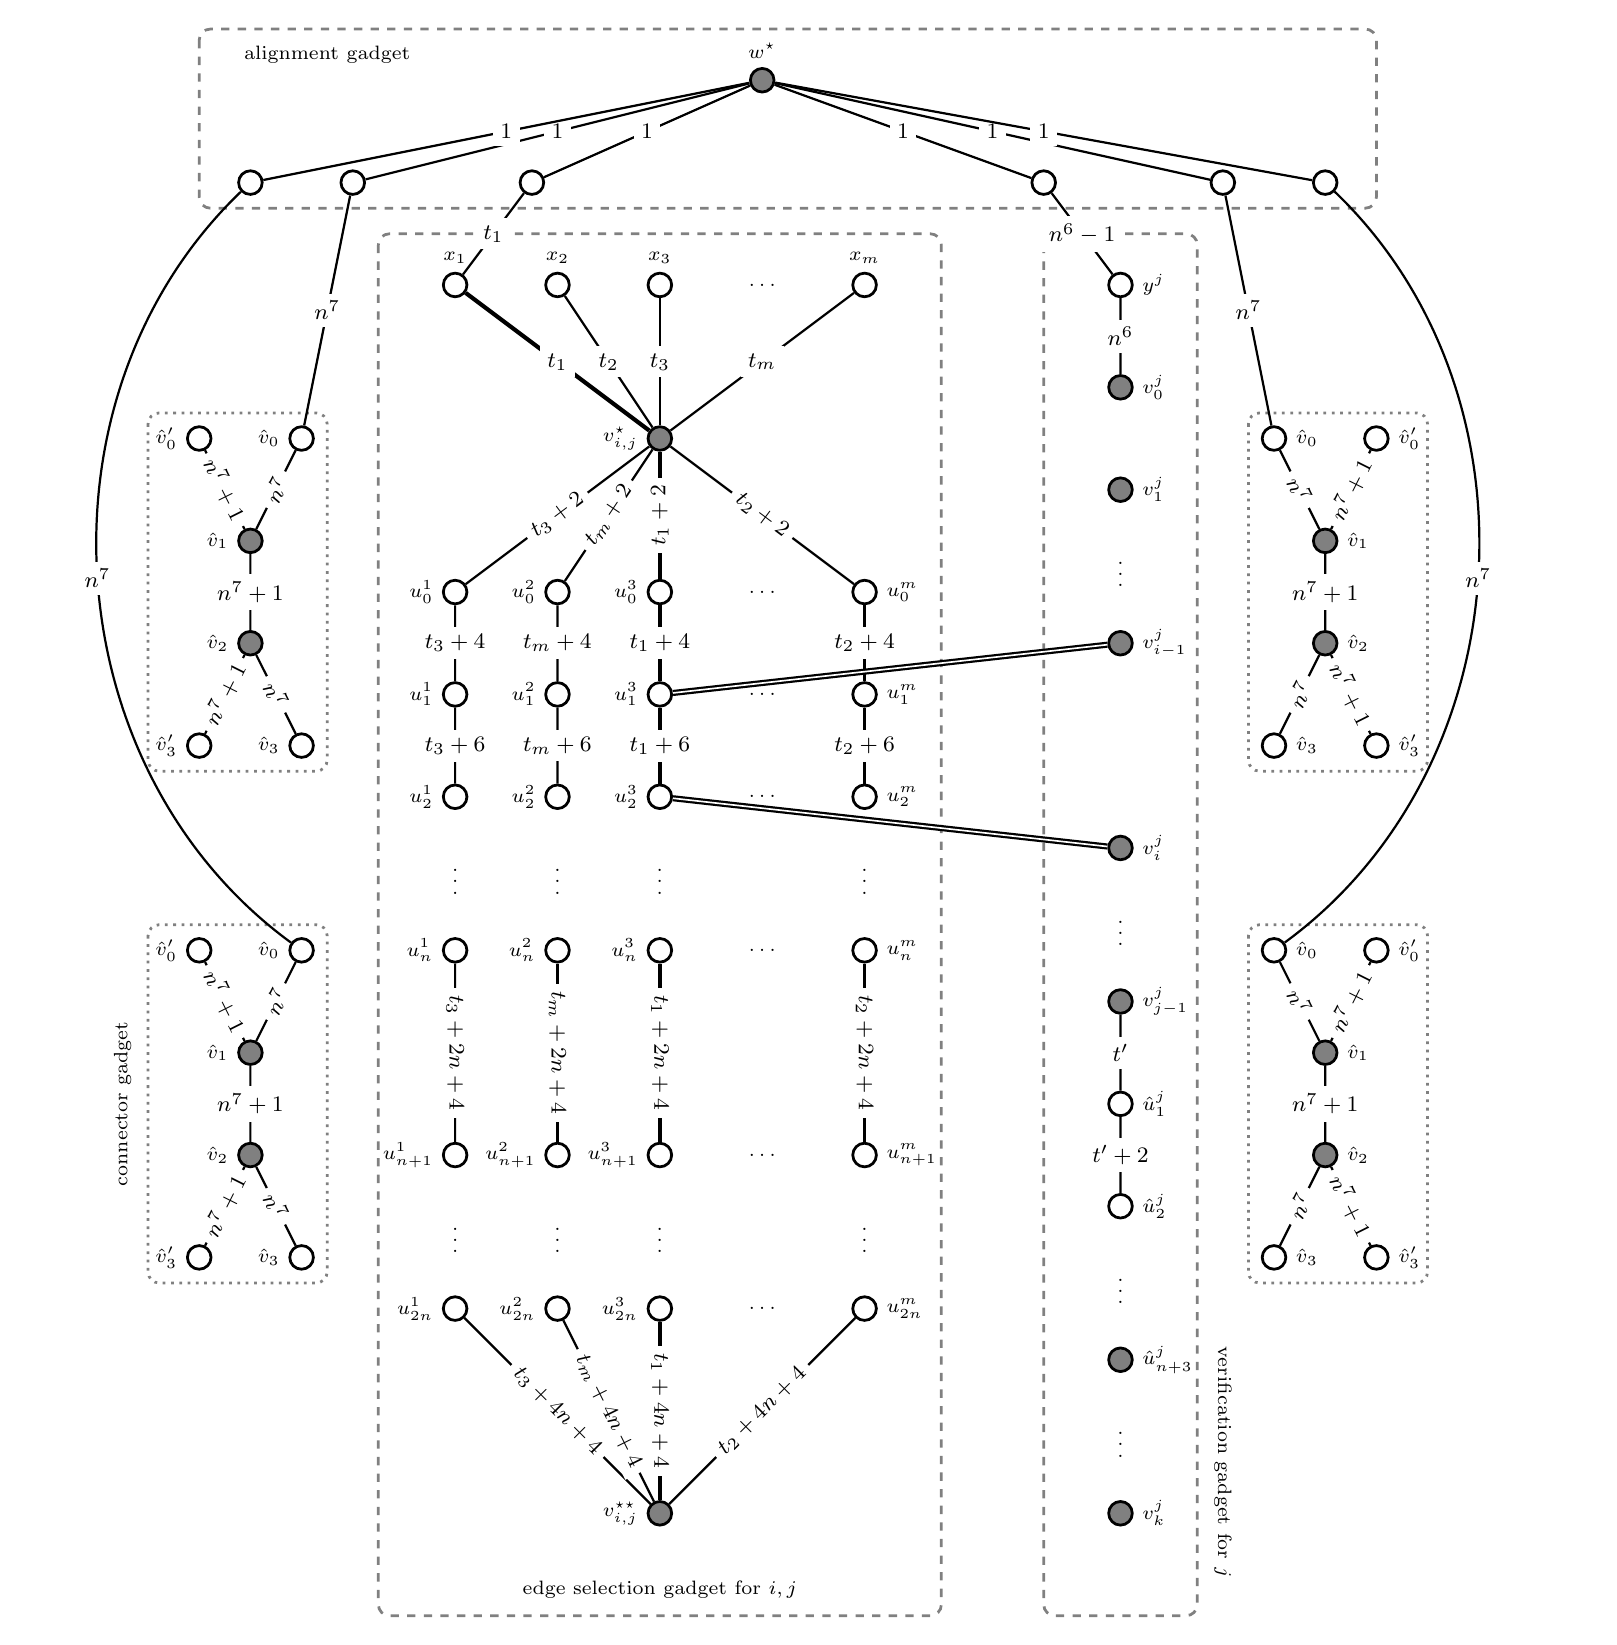
\begin{tikzpicture}[line width=1pt, scale=.65]
\scriptsize
\node (A) at (14,0) {};

\draw[rounded corners, dashed, gray] (-13, 5) rectangle (10, 1.5) {};
\node (A) at (-10.5,4.5) {alignment gadget};

\draw[rounded corners, dotted, gray] (-14, -2.5) rectangle (-10.5, -9.5) {};
\draw[rounded corners, dotted, gray] (-14, -12.5) rectangle (-10.5, -19.5) {};
\draw[rounded corners, dotted, gray] (7.5, -2.5) rectangle (11, -9.5) {};
\draw[rounded corners, dotted, gray] (7.5, -12.5) rectangle (11, -19.5) {};
\node[rotate=90] (A) at (-14.5,-16) {connector gadget};

\draw[rounded corners, dashed, gray] (-9.5, 1) rectangle (1.5, -26) {};
\node (A) at (-4,-25.5) {edge selection gadget for $i,j$};

\draw[rounded corners, dashed, gray] (3.5, 1) rectangle (6.5, -26) {};
\node[rotate=-90] (A) at (7,-23) {verification gadget for $j$};

    \node[vert,label=above:$w^\star$, fill=gray] (W) at (-2,4) {};
    \node[vert] (W1) at (-6.5,2) {};
    \node[vert] (W2) at (-10,2) {};
    \node[vert] (W3) at (-12,2) {};
    \node[vert] (W4) at (7,2) {}; 
    \node[vert] (W5) at (3.5,2) {};
    \node[vert] (W6) at (9,2) {}; 


    \node[vert,label=left:$\hat{v}_0$] (VH11) at (-11,-3) {}; 
    \node[vert,label=left:$\hat{v}_0'$] (VH111) at (-13,-3) {}; 
    \node[vert,label=left:$\hat{v}_1$, fill=gray] (VH12) at (-12,-5) {}; 
    \node[vert,label=left:$\hat{v}_2$, fill=gray] (VH13) at (-12,-7) {}; 
    \node[vert,label=left:$\hat{v}_3$] (VH14) at (-11,-9) {};  
    \node[vert,label=left:$\hat{v}_3'$] (VH144) at (-13,-9) {}; 

    \node[vert,label=left:$\hat{v}_0$] (VH21) at (-11,-13) {};
    \node[vert,label=left:$\hat{v}_0'$] (VH211) at (-13,-13) {}; 
    \node[vert,label=left:$\hat{v}_1$, fill=gray] (VH22) at (-12,-15) {}; 
    \node[vert,label=left:$\hat{v}_2$, fill=gray] (VH23) at (-12,-17) {};
    \node[vert,label=left:$\hat{v}_3$] (VH24) at (-11,-19) {};
    \node[vert,label=left:$\hat{v}_3'$] (VH244) at (-13,-19) {}; 

    \node[vert,label=right:$\hat{v}_0$] (VH31) at (8,-3) {}; 
    \node[vert,label=right:$\hat{v}_0'$] (VH311) at (10,-3) {}; 
    \node[vert,label=right:$\hat{v}_1$, fill=gray] (VH32) at (9,-5) {}; 
    \node[vert,label=right:$\hat{v}_2$, fill=gray] (VH33) at (9,-7) {}; 
    \node[vert,label=right:$\hat{v}_3$] (VH34) at (8,-9) {};  
    \node[vert,label=right:$\hat{v}_3'$] (VH344) at (10,-9) {}; 

    \node[vert,label=right:$\hat{v}_0$] (VH41) at (8,-13) {}; 
    \node[vert,label=right:$\hat{v}_0'$] (VH411) at (10,-13) {}; 
    \node[vert,label=right:$\hat{v}_1$, fill=gray] (VH42) at (9,-15) {}; 
    \node[vert,label=right:$\hat{v}_2$, fill=gray] (VH43) at (9,-17) {}; 
    \node[vert,label=right:$\hat{v}_3$] (VH44) at (8,-19) {};  
    \node[vert,label=right:$\hat{v}_3'$] (VH444) at (10,-19) {}; 
    
    \node[vert,label=above:$x_1$] (X1) at (-8,0) {}; 
    \node[vert,label=above:$x_2$] (X2) at (-6,0) {}; 
    \node[vert,label=above:$x_3$] (X3) at (-4,0) {}; 
    \node (A) at (-2,0) {$\ldots$};
    \node[vert,label=above:$x_m$] (XM) at (0,0) {}; 
    
    \node[vert,label=left:$v_{i,j}^\star$, fill=gray] (VS) at (-4,-3) {}; 
    
    \node[vert,label=left:$u^1_0$] (Y1) at (-8,-6) {}; 
    \node[vert,label=left:$u^2_0$] (Y2) at (-6,-6) {}; 
    \node[vert,label=left:$u^3_0$] (Y3) at (-4,-6) {}; 
    \node (A) at (-2,-6) {$\ldots$};
    \node[vert,label=right:$u^m_0$] (YM) at (0,-6) {}; 

    \node[vert,label=left:$u^1_1$] (U11) at (-8,-8) {}; 
    \node[vert,label=left:$u^2_1$] (U12) at (-6,-8) {}; 
    \node[vert,label=left:$u^3_1$] (U13) at (-4,-8) {}; 
    \node (A) at (-2,-8) {$\ldots$};
    \node[vert,label=right:$u^m_1$] (U1M) at (0,-8) {};
    
    \node[vert,label=left:$u^1_2$] (U21) at (-8,-10) {}; 
    \node[vert,label=left:$u^2_2$] (U22) at (-6,-10) {}; 
    \node[vert,label=left:$u^3_2$] (U23) at (-4,-10) {}; 
    \node (A) at (-2,-10) {$\ldots$};
    \node[vert,label=right:$u^m_2$] (U2M) at (0,-10) {};
    
    \node (A) at (-8,-11.5) {$\vdots$}; 
    \node (A) at (-6,-11.5) {$\vdots$}; 
    \node (A) at (-4,-11.5) {$\vdots$}; 
    \node (A) at (0,-11.5) {$\vdots$};

    \node[vert,label=left:$u^1_n$] (UN1) at (-8,-13) {}; 
    \node[vert,label=left:$u^2_n$] (UN2) at (-6,-13) {}; 
    \node[vert,label=left:$u^3_n$] (UN3) at (-4,-13) {}; 
    \node (A) at (-2,-13) {$\ldots$};
    \node[vert,label=right:$u^m_n$] (UNM) at (0,-13) {};

    \node[vert,label=left:$u_{n+1}^1$] (UN11) at (-8,-17) {}; 
    \node[vert,label=left:$u_{n+1}^2$] (UN12) at (-6,-17) {}; 
    \node[vert,label=left:$u_{n+1}^3$] (UN13) at (-4,-17) {}; 
    \node (A) at (-2,-17) {$\ldots$};
    \node[vert,label=right:$u_{n+1}^m$] (UN1M) at (0,-17) {};
        
    \node (A) at (-8,-18.5) {$\vdots$}; 
    \node (A) at (-6,-18.5) {$\vdots$}; 
    \node (A) at (-4,-18.5) {$\vdots$}; 
    \node (A) at (0,-18.5) {$\vdots$};

    \node[vert,label=left:$u_{2n}^1$] (U2N1) at (-8,-20) {}; 
    \node[vert,label=left:$u_{2n}^2$] (U2N2) at (-6,-20) {}; 
    \node[vert,label=left:$u_{2n}^3$] (U2N3) at (-4,-20) {}; 
    \node (A) at (-2,-20) {$\ldots$};
    \node[vert,label=right:$u_{2n}^m$] (U2NM) at (0,-20) {};
    
    \node[vert,label=left:$v_{i,j}^{\star\star}$, fill=gray] (VSS) at (-4,-24) {};


    \node[vert,label=right:$y^j$] (YI) at (5,0) {};
    \node[vert,label=right:$v_0^j$, fill=gray] (VI0) at (5,-2) {};
    \node[vert,label=right:$v_1^j$, fill=gray] (VI1) at (5,-4) {};
    \node (A) at (5,-5.5) {$\vdots$};
    \node[vert,label=right:$v_{i-1}^j$, fill=gray] (VIJ1) at (5,-7) {};
    \node[vert,label=right:$v_{i}^j$, fill=gray] (VIJ) at (5,-11) {};
    \node (A) at (5,-12.5) {$\vdots$};
    \node[vert,label=right:$v_{j-1}^j$, fill=gray] (VII1) at (5,-14) {};
    \node[vert,label=right:$\hat{u}_{1}^j$] (UI1) at (5,-16) {};
    \node[vert,label=right:$\hat{u}_{2}^j$] (UI2) at (5,-18) {};
    \node (A) at (5,-19.5) {$\vdots$};
    \node[vert,label=right:$\hat{u}_{n+3}^j$, fill=gray] (UIN3) at (5,-21) {};
    \node (A) at (5,-22.5) {$\vdots$};
    \node[vert,label=right:$v_{k}^j$, fill=gray] (VIK) at (5,-24) {};
    
	\draw[edge, line width=1.5pt] (X1) --node[timelabel] {$t_1$} (VS);
	\draw[edge] (X2) --node[timelabel] {$t_2$} (VS);
	\draw[edge] (X3) --node[timelabel] {$t_3$} (VS);
	\draw[edge] (XM) --node[timelabel] {$t_m$} (VS);

    \draw[edge] (Y1) --node[timelabel,sloped] {$t_3+2$} (VS);
	\draw[edge] (Y2) --node[timelabel,sloped] {$t_m+2$} (VS);
	\draw[edge, line width=1.5pt] (Y3) --node[timelabel,sloped] {$t_1+2$} (VS);
	\draw[edge] (YM) --node[timelabel,sloped] {$t_2+2$} (VS);

    \draw[edge] (Y1) --node[timelabel] {$t_3+4$} (U11);
	\draw[edge] (Y2) --node[timelabel] {$t_m+4$} (U12);
	\draw[edge, line width=1.5pt] (Y3) --node[timelabel] {$t_1+4$} (U13);
	\draw[edge] (YM) --node[timelabel] {$t_2+4$} (U1M);
	
    \draw[edge] (U21) --node[timelabel] {$t_3+6$} (U11);
	\draw[edge] (U22) --node[timelabel] {$t_m+6$} (U12);
	\draw[edge, line width=1.5pt] (U23) --node[timelabel] {$t_1+6$} (U13);
	\draw[edge] (U2M) --node[timelabel] {$t_2+6$} (U1M);

    \draw[edge] (UN1) --node[timelabel,sloped] {$t_3+2n+4$} (UN11);
	\draw[edge] (UN2) --node[timelabel,sloped] {$t_m+2n+4$} (UN12);
	\draw[edge, line width=1.5pt] (UN3) --node[timelabel,sloped] {$t_1+2n+4$} (UN13);
	\draw[edge] (UNM) --node[timelabel,sloped] {$t_2+2n+4$} (UN1M);
 
    \draw[edge] (U2N1) --node[timelabel,sloped] {$t_3+4n+4$} (VSS);
	\draw[edge] (U2N2) --node[timelabel,sloped] {$t_m+4n+4$} (VSS);
	\draw[edge, line width=1.5pt] (U2N3) --node[timelabel,sloped] {$t_1+4n+4$} (VSS);
	\draw[edge] (U2NM) --node[timelabel,sloped] {$t_2+4n+4$} (VSS);

    \draw[edge] (VH11) --node[timelabel,sloped] {$n^7$} (VH12);
	\draw[edge] (VH12) --node[timelabel,sloped] {$n^7+1$} (VH111);
	\draw[edge] (VH12) --node[timelabel] {$n^7+1$} (VH13);
    \draw[edge] (VH13) --node[timelabel,sloped] {$n^7$} (VH14);
	\draw[edge] (VH13) --node[timelabel,sloped] {$n^7+1$} (VH144);
	
    \draw[edge] (VH21) --node[timelabel,sloped] {$n^7$} (VH22);
	\draw[edge] (VH22) --node[timelabel,sloped] {$n^7+1$} (VH211);
	\draw[edge] (VH22) --node[timelabel] {$n^7+1$} (VH23);
    \draw[edge] (VH23) --node[timelabel,sloped] {$n^7$} (VH24);
	\draw[edge] (VH23) --node[timelabel,sloped] {$n^7+1$} (VH244);
 
    \draw[edge] (VH31) --node[timelabel,sloped] {$n^7$} (VH32);
	\draw[edge] (VH32) --node[timelabel,sloped] {$n^7+1$} (VH311);
	\draw[edge] (VH32) --node[timelabel] {$n^7+1$} (VH33);
    \draw[edge] (VH33) --node[timelabel,sloped] {$n^7$} (VH34);	
    \draw[edge] (VH33) --node[timelabel,sloped] {$n^7+1$} (VH344);

    \draw[edge] (VH41) --node[timelabel,sloped] {$n^7$} (VH42);
	\draw[edge] (VH42) --node[timelabel,sloped] {$n^7+1$} (VH411);
	\draw[edge] (VH42) --node[timelabel] {$n^7+1$} (VH43);
    \draw[edge] (VH43) --node[timelabel,sloped] {$n^7$} (VH44);	
    \draw[edge] (VH43) --node[timelabel,sloped] {$n^7+1$} (VH444);
 
	%\draw[edge] (VIJ1) --node[timelabel, near start] {$t_1+4$} (U13);
	%\draw[edge] (VIJ) --node[timelabel, near start] {$t_1+8$} (U23);

    \draw[edge,double] (VIJ1) --node {} (U13);
	\draw[edge,double] (VIJ) --node {} (U23);
 
 
	\draw[edge] (W) --node[timelabel] {$1$} (W1);
	\draw[edge] (W) --node[timelabel] {$1$} (W2);
	\draw[edge] (W) --node[timelabel] {$1$} (W3);
	\draw[edge] (W) --node[timelabel] {$1$} (W4);
	\draw[edge] (W) --node[timelabel] {$1$} (W5);
	\draw[edge] (W) --node[timelabel] {$1$} (W6);
 
	\draw[edge] (X1) --node[timelabel] {$t_1$} (W1);
	\draw[edge] (VH11) --node[timelabel] {$n^7$} (W2);
	\draw[edge] (VH21) edge[bend left=50] node[timelabel] {$n^7$} (W3);
	\draw[edge] (VH31) --node[timelabel] {$n^7$} (W4);
	\draw[edge] (YI) --node[timelabel] {$n^6-1$} (W5);
	\draw[edge] (VH41) edge[bend right=50] node[timelabel] {$n^7$} (W6);

	\draw[edge] (YI) --node[timelabel] {$n^6$} (VI0);
 
	\draw[edge] (VII1) --node[timelabel] {$t'$} (UI1);
	\draw[edge] (UI1) --node[timelabel] {$t'+2$} (UI2);
\end{tikzpicture}
    %\end{center}
    }
    \caption{Illustration of part of the underlying graph $G$ and a possible labelling. Edges incident with vertices of connector gadgets are omitted. Gray vertices form a feedback vertex set.}\label{fig:hardness1}
\end{figure}


\subparagraph{Correctness.} This finishes the construction of \deltaExactLong\ instance, which can clearly be computed in polynomial time. For an illustration see \cref{fig:hardness1}. As discussed earlier, we have that the vertex cover number of the underlying graph of the instance is in $O(k^2)$.

In the remainder we prove that $D$ is a yes-instance of \deltaExactLong\ if and only if the $H$ is a yes-instance of \textsc{Multicolored Clique}.

\subparagraph{$(\Rightarrow)$:} Assume $D$ is a yes-instance of \deltaExactLong\ and let $(G,\lambda)$ be a solution. We have that the underlying graph $G$ is uniquely defined by $D$. We first prove a number of properties of $\lambda$ that we need to define a set of vertices in $H$ which we claim to be a multicolored clique.

To start, consider the alignment gadget. We can observe that all edges incident with $w^\star$ have the same label.
\begin{claim}\label{claim:1}
    For all $w\in \hat{W}$ we have that $\lambda(\{w^\star,w\})=t$ for some $t\in\mathbb{N}$.
\end{claim}
\begin{claimproof}
    Assume for contradiction that there are $w,w'\in \hat{W}$ such that $\lambda(\{w^\star,w\})=t$ and $\lambda(\{w^\star,w'\})=t'$ with $t\neq t'$. Let w.l.o.g.\ $t<t'$. Then $w$ can reach $w'$, however we have that $d(w,w')=\infty$, a contradiction.
\end{claimproof}
\cref{claim:1} allows us to assume w.l.o.g.\ that all edges incident with vertex $w^\star$ of the alignment gadget have label $1$. From now we will assume that this is the case.

Next, we analyse the labelings of connector gadgets. We show that all edges incident with vertices of connector gadgets have labels of at least $n^7$ and at most $n^7+2$. More precisely, we show the following.
\begin{claim}\label{claim:2}
    Let $\hat{v}_0,\hat{v}_0',\hat{v}_1,\hat{v}_2,\hat{v}_3,\hat{v}_3'$ be the vertices of a connector gadget with sets $A$ and $B$. Then we have that 
    %\begin{itemize}
        %\item 
        $\lambda(\{\hat{v}_0,\hat{v}_1\})=n^7$,  $\lambda(\{\hat{v}_0',\hat{v}_1\})=n^7+2$,
        %\item 
        $\lambda(\{\hat{v}_1,\hat{v}_2\})=n^7+1$, $\lambda(\{\hat{v}_2,\hat{v}_3\})=n^7$, and $\lambda(\{\hat{v}_2,\hat{v}_3'\})=n^7+2$. 
        %\item For all $v\in V^\star$ we have $n^7\le \lambda(\{\hat{v}_1,v\}), \lambda(\{\hat{v}_2,v\})\le n^7+2$.
        %\item For all $v\in A\setminus B$ we have $\lambda(\{\hat{v}_1,v\})=n^7$ and $\lambda(\{\hat{v}_2,v\})=n^7+2$.
        %\item For all $v\in B$ we have $\lambda(\{\hat{v}_1,v\})=n^7$ and $\lambda(\{\hat{v}_2,v\})=n^7$.
        %\item 
        Furthermore, for all $v\in V^\star$ we have $n^7\le \lambda(\{\hat{v}_1,v\})\le n^7+2$ and $n^7\le \lambda(\{\hat{v}_2,v\}) \le n^7+2$.
    %\end{itemize}
\end{claim}
\begin{claimproof}
    Let $w\in \hat{W}$ denote the vertex of the alignment gadget that is neighbor of $w^\star$ and $\hat{v}_0$. We have $d(w^\star,\hat{v}_0)=n^7$. It follows that $\lambda(\{w,\hat{v}_0\})=n^7$. Since $d(\hat{v}_1,w)=\infty$ and $d(w,\hat{v}_1)=\infty$, we have that $\lambda(\{\hat{v}_0,\hat{v}_1\})=n^7$.
    Note that $\hat{v}_1$ is the only common neighbor of $\hat{v}_0$ and $\hat{v}_2$ and the only common neighbor of $\hat{v}_0$ and $\hat{v}_0'$. Since $d(\hat{v}_0,\hat{v}_2)=2$ and $d(\hat{v}_0,\hat{v}_0')=3$ we have that $\lambda(\{\hat{v}_1,\hat{v}_2\})=n^7+1$ and $\lambda(\{\hat{v}_0',\hat{v}_1\})=n^7+2$. Similarly, we have that $\hat{v}_2$ is the only common neighbor of $\hat{v}_3$ and $\hat{v}_1$ and the only common neighbor of $\hat{v}_3$ and $\hat{v}_3'$. Since $d(\hat{v}_3,\hat{v}_1)=2$ and $d(\hat{v}_3,\hat{v}_3')=3$ we have that $\lambda(\{\hat{v}_2,\hat{v}_3\})=n^7$ and $\lambda(\{\hat{v}_2,\hat{v}_3'\})=n^7+2$.

%    
Let $v\in V^\star$. Note that $d(v,\hat{v}_0)=\infty$ and $d(v,\hat{v}_3)=\infty$. It follows that $\lambda(\{\hat{v}_1,v\})\ge n^7$ and $\lambda(\{\hat{v}_2,v\})\ge n^7$. Otherwise, there would be a temporal path from $v$ to $\hat{v}_0$ via $\hat{v}_1$ or a temporal path from $v$ to $\hat{v}_3$ via $\hat{v}_2$, a contradiction.
Furthermore, note that $d(\hat{v}_0',v)=\infty$ and $d(\hat{v}_3',v)=\infty$. It follows that $\lambda(\{\hat{v}_1,v\})\le n^7+2$ and $\lambda(\{\hat{v}_2,v\})\le n^7+2$. Otherwise, there would be a temporal path from $\hat{v}_0'$ to $v$ via $\hat{v}_1$ or a temporal path from $\hat{v}_3$ to $v$ via $\hat{v}_2$, a contradiction.
%Furthermore, if $v\in B$ then we also have $d(\hat{v}_0,v)=\infty$ and it follows that $\lambda(\{\hat{v}_1,v\})=n^7$.
%If $v\notin B$ then we have $d(\hat{v}_0,v)=3$ and it follows that $\lambda(\{\hat{v}_1,v\})=n^7+2$ or $\lambda(\{\hat{v}_2,v\})=n^7+2$.
\end{claimproof}

Now we take a closer look at the edge selection gadgets. We make a number of observations that will allow us to define a set of vertices in $H$ that we claim to be a multicolored clique.

\begin{claim}\label{claim:3}
    For all $1\le i<j\le k$ and $\ell\in[m]$ we have that $\lambda(\{u_\ell^{2n},v_{i,j}^{\star\star}\})\le n^7+2$, where $u_\ell^{2n}$ belongs to the edge selection gadget for $i,j$.
\end{claim}
\begin{claimproof}
    Consider the first connector gadget of the edge selection gadget for $i,j$ with vertices $\hat{v}_0,\hat{v}_0',\hat{v}_1,\hat{v}_2,\hat{v}_3,\hat{v}_3'$ and sets $A,B$. Recall that $v_{i,j}^{\star\star}\in B$ and hence we have that $d(\hat{v}_0,v_{i,j}^{\star\star})=\infty$. Furthermore, we have that $u_\ell^{2n}\notin B$ and hence $d(\hat{v}_0,u_\ell^{2n})=3$. By \cref{claim:2} and the fact that $d(w^\star,\hat{v}_0)=n^7$ we have that both edges incident with $\hat{v}_0$ have label $n^7$. It follows that a fastest temporal path from $\hat{v}_0$ to $u_\ell^{2n}$ arrives at $u_\ell^{2n}$ at time $n^7+2$. Now assume for contradiction that $\lambda(\{u_\ell^{2n},v_{i,j}^{\star\star}\})> n^7+2$. Then there exists a temporal walk from $\hat{v}_0$ to $v_{i,j}^{\star\star}$ via $u_\ell^{2n}$, a contradiction to $d(\hat{v}_0,v_{i,j}^{\star\star})=\infty$.
\end{claimproof}

\begin{claim}\label{claim:4}
    For all $1\le i<j\le k$ and $\ell\in[m]$ we have that $\lambda(\{x_\ell,v_{i,j}^{\star}\})=(i+j)\cdot (2n\ell +18n+2)$, where $x_\ell$ belongs to the edge selection gadget for $i,j$.
\end{claim}
\begin{claimproof}
    We first determine the label of $\{x_1,v_{i,j}^{\star}\}$, where $x_1$ belongs to the edge selection gadget for $i,j$. Note that $x_1$ is connected to the alignment gadget. Let $w\in \hat{W}$ be the vertex of the alignment gadget that is a neighbor of $x_1$. Since $d(w^\star,x_1)=(20n+2)(i+j)$ we have that $\lambda(\{w,x_1\})=(20n+2)(i+j)$. 

    First, assume that $\lambda(\{x_1,v_{i,j}^{\star}\})<(20n+2)(i+j)$. Then there is a temporal path from $v_{i,j}^\star$ to $w$ via $x_1$. However, we have that $d(x_{i,j^\star},w)=\infty$, a contradiction.
    Next, assume that $(20n+2)(i+j)<\lambda(\{x_1,v_{i,j}^{\star}\})<n^7+2$. Then there is a temporal path from $w$ to $v_{i,j}$ via $x_1$ with duration strictly less than $n^7-(20n+2)(i+j)+3$. However, we have that $d(w,v_{i,j}^\star)=n^7-(20n+2)(i+j)+3$, a contradiction.
    Finally, assume that $\lambda(\{x_1,v_{i,j}^{\star}\})\ge n^7+2$. Consider a fastest temporal path from $x_1$ to $v_{i,j}^{\star\star}$. This temporal path cannot visit $w$ as its first vertex, since from there it cannot continue. It follows by \cref{claim:2} and the just made assumption that the first edge of the temporal path has a label of at least $n^7$. However, by \cref{claim:2,claim:3} we have that all edges incident with $v_{i,j}^{\star\star}$ have a label of at most $n^7+2$. It follows that $d(x_1,v_{i,j}^{\star\star})\le 3$, a contradiction.

    We can conclude that $\lambda(\{x_1,v_{i,j}^{\star}\})=(20n+2)(i+j)$. Now let $1<\ell\le m$. We have that $d(x_1,x_\ell)=2n\cdot (i+j)\cdot(\ell-1)+1$ which implies that $\lambda(\{x_\ell,v_{i,j}^{\star}\})\ge (i+j)\cdot (2n\ell +18n+2)$. Assume that $(i+j)\cdot (2n\ell +18n+2) <\lambda(\{x_\ell,v_{i,j}^{\star}\})\le n^7+2$. Then the temporal path from $x_1$ to $x_\ell$ via $v_{i,j}^\star$ is not a fastest temporal path from $x_1$ to $x_\ell$. Again, we have that a fastest temporal path from $x_1$ to $x_\ell$ cannot visit $w$ as its first vertex, since from there it cannot continue. By \cref{claim:2}, all other edges incident with $x_1$ (that is, all different from the one to $v_{i,j}^\star$ and the one to $w$) have a label of at least $n^7$ and at most $n^7+2$. Similarly, by \cref{claim:2} we have that all other edges incident with $x_\ell$ (that is, all different from the one to $v_{i,j}^\star$) have a label of at least $n^7$ and at most $n^7+2$. It follows that any temporal path from $x_1$ to $x_\ell$ that visits $v_{i,j}^\star$ as its first vertex has a duration strictly larger than $2n\cdot (i+j)\cdot(\ell-1)+1$. Any temporal path from $x_1$ to $x_\ell$ that visits a vertex different from $v_{i,j}^\star$ as its first vertex has duration of at most $3$. In both cases we have a contradiction. 
    Lastly, assume that $\lambda(\{x_\ell,v_{i,j}^{\star}\})> n^7+2$. Consider a fastest temporal path from $x_\ell$ to $v_{i,j}^{\star\star}$. Now this temporal path has duration at most 3 since by \cref{claim:2} and the just made assumption all edges incident with $x_\ell$ have label at least $n^7$ whereas by \cref{claim:2,claim:3} all edges incident with $v_{i,j}^{\star\star}$ have label at most $n^7+2$, a contradiction. 
\end{claimproof}

\begin{claim}\label{claim:5}
    For all $1\le i<j\le k$ there exist a permutation $\sigma_{i,j}:[m]\rightarrow [m]$ such that for all $\ell\in[m]$ we have that $\lambda(\{u_\ell^{2n},v_{i,j}^{\star\star}\})=(i+j)\cdot (2n\cdot \sigma_{i,j}(\ell) +18n+2)+4n+4$, where $u_\ell^{2n}$ belongs to the edge selection gadget for $i,j$.

    Furthermore, a fastest temporal path from $x_\ell$ (of the edge selection gadget for $i,j$) to $v_{i,j}^{\star\star}$ visits $v_{i,j}^\star$ as its second vertex, and $u_{\ell'}^{2n}$ with $\sigma_{i,j}(\ell')=\ell$ (of the edge selection gadget for $i,j$) as its second last vertex.
\end{claim}
\begin{claimproof}
    For every $\ell\in[m]$ we have that $d(x_\ell,v_{i,j}^{\star\star})=4n+5$, where $x_\ell$ belongs to the edge selection gadget for $i,j$. From \cref{claim:2,claim:4} follows that all edges incident with $x_\ell$ have a label of at least $n^7$ except the one to $v_{i,j}^\star$ and, if $\ell=1$, the edge connecting $x_1$ to the alignment gadget. In the latter case, no temporal path from $x_1$ from $v_{i,j}^{\star\star}$ can continue to the neighbor of $x_1$ in the alignment gadget, since it cannot continue from there.

    Now consider $v_{i,j}^{\star\star}$. By \cref{claim:2,claim:3} we have that all edges incident with $v_{i,j}^{\star\star}$ have a label of at most $n^7+2$. It follows that a fastest temporal path $P$ from $x_\ell$ to $v_{i,j}^{\star\star}$ has to visit $v_{i,j}^\star$ after $x_\ell$, since otherwise we have $d(x_\ell,v_{i,j}^{\star\star})\le 2$, a contradiction.

    Furthermore, we have by \cref{claim:2} that all edges incident with $v_{i,j}^{\star\star}$ have a label of at least $n^7$ except the ones to $u_{\ell'}^{2n}$ for $\ell'\in[m]$. By \cref{claim:4} we have that $\lambda(\{x_\ell,v_{i,j}^{\star}\})\le 4n^4$.
    It follows that a fastest temporal path from $x_\ell$ to $v_{i,j}^{\star\star}$ has to visit $u_{\ell'}^{2n}$ for some $\ell'\in[m]$ as its second last vertex. Otherwise, we have $d(x_\ell,v_{i,j}^{\star\star})> 4n+5$ (for sufficiently large $n$), a contradiction.

    We can conclude that a fastest temporal path from $x_\ell$ to $v_{i,j}^{\star\star}$ has to visit $v_{i,j}^\star$ as its second vertex and $u_{\ell'}^{2n}$ for some $\ell'\in[m]$ as its second last vertex. Recall that in a  temporal path, the difference between the labels of the first and last edge determine its duration (minus one). Hence, we have that $\lambda(\{u_{\ell'}^{2n},v_{i,j}^{\star\star}\})-\lambda(\{x_\ell,v_{i,j}^{\star}\})+1=4n+5$.
    By \cref{claim:4} we have that $\lambda(\{x_\ell,v_{i,j}^{\star}\})=(i+j)\cdot (2n\ell+18n +2)$. It follows that $\lambda(\{u_{\ell'}^{2n},v_{i,j}^{\star\star}\})=(i+j)\cdot (2n\ell +18n+2)+4n+4$. We set $\sigma_{i,j}(\ell')=\ell$.

    Finally, we show that $\sigma_{i,j}$ is a permutation on $[m]$. Assume for contradiction that there are $\ell,\ell'\in[m]$ with $\ell\neq \ell'$ such that $\sigma_{i,j}(\ell)=\sigma_{i,j}(\ell')$. Then we have that $\lambda(\{u_{\ell}^{2n},v_{i,j}^{\star\star}\})=\lambda(\{u_{\ell'}^{2n},v_{i,j}^{\star\star}\})$. However, by \cref{claim:4} we have that all edges from $v_{i,j}$ to a vertex in $X_{i,j}$ have distinct labels. Furthermore, we argued above that every fastest path from a vertex in $X_{i,j}$ to $v_{i,j}^{\star\star}$ visits $v_{i,j}^\star$ as its second vertex and a vertex from the set $\{u_{\ell''}^{2n}\mid \ell''\in[m]\}$ as its second last vertex. Since for all $x_{\ell''}$ with $\ell''\in[m]$ we have that $d(x_{\ell''},v_{i,j}^{\star\star})=4n+5$, we must have that all edges from vertices in $\{u_{\ell''}^{2n}\mid \ell''\in[m]\}$ to $v_{i,j}^{\star\star}$ must have distinct labels. Hence, we have a contradiction and can conclude that $\sigma_{i,j}$ is indeed a permutation.
\end{claimproof}

For all $1\le i<j\le k$, let $\sigma_{i,j}$ be the permutation on $[m]$ as defined in \cref{claim:5}. We call $\sigma_{i,j}$ the \emph{permutation of color combination $i,j$}. 
Now we have enough information to define a set of vertices of $H$ that form a multicolored clique.
To this end, consider the following set $X$ of edges from $H$.
\[
X=\{e_\ell^{i,j}\in F_{i,j}\mid \sigma_{i,j}(\ell)=1\}
\]
We claim that $\bigcup_{e\in X}e$ forms a multicolored clique in $H$.
From now on, denote $\{e_{i,j}\}=X\cap F_{i,j}$. We show that for all $i\in [k]$ we have that $|(\bigcap_{1\le j<i} e_{j,i}) \cap (\bigcap_{i<j\le k} e_{i,j})|=1$, that is, for every color~$i$, all edges of a color combination involving $i$ have the same vertex of color $i$ as endpoint. This implies that $\bigcup_{e\in X}e$ is a multicolored clique in $H$.

Before we proceed, we show some further properties of $\lambda$. First, we have a closer look at the labels on edges of the edge selection gadgets.

\begin{claim}\label{claim:6}
    For all $1\le i<j\le k$,  $\ell\in[m]$, and $\ell'\in[2n]$ we have that $\lambda(\{u^\ell_{\ell'-1},u^\ell_{\ell'}\})=(i+j)\cdot (2n\cdot \sigma_{i,j}(\ell) +18n+2)+2\ell'+2$, where $u^\ell_{\ell'-1}$ and $u^\ell_{\ell'}$ belong to the edge selection gadget for $i,j$ and $\sigma_{i,j}$ is the permutation of color combination $i,j$.
\end{claim}
\begin{claimproof}
    Let $1\le i<j\le k$ and $\ell\in[m]$.
    By \cref{claim:5} we know that a fastest temporal path from $x_{\sigma_{i,j}(\ell)}$ (of the edge selection gadget for $i,j$) to $v_{i,j}^{\star\star}$ visits $v_{i,j}^\star$ as its second vertex, and $u_{\ell}^{2n}$ (of the edge selection gadget for $i,j$) as its second last vertex. 
    Furthermore, by \cref{claim:4} we have that $\lambda(\{x_{\sigma_{i,j}(\ell)},v_{i,j}^{\star}\})=(i+j)\cdot (2n\cdot {\sigma_{i,j}(\ell)}+18n +2)$ and by \cref{claim:5} we have that $\lambda(\{u_\ell^{2n},v_{i,j}^{\star\star}\})=(i+j)\cdot (2n\cdot \sigma_{i,j}(\ell)+18n +2)+4n+4$. It follows that there exist a temporal path $P$ from $v_{i,j}^\star$ to $u_\ell^{2n}$ that starts at $v_{i,j}^\star$ later than $(i+j)\cdot (2n\cdot {\sigma_{i,j}(\ell)} +18n+2)$ and arrives at $u_\ell^{2n}$ earlier than $(i+j)\cdot (2n\cdot \sigma_{i,j}(\ell) +18n+2)+4n+4$. Hence, the temporal path $P$ has duration at most $4n+3$.

    We investigate the temporal path $P$ from its destination $u_\ell^{2n}$ back to its start vertex $v_{i,j}^\star$. Consider the neighbors of $u_\ell^{2n}$ that are different from $v_{i,j}^{\star\star}$. By \cref{claim:2} we have that all edges from $u_\ell^{2n}$ to neighbors of $u_\ell^{2n}$ that are vertices of connector gadgets have a label of at least $n^7$. Hence, $P$ does not visit any of those neighbors. Next, consider neighbors of $u_\ell^{2n}$ is verification gadgets. Assume $u_\ell^{2n}$ has a neighbor in the verification gadget of color $i'$ for some $i'\in[k]$. Then this neighbor is vertex $b^{i',j,\ell}_{5n}$. Note that if $P$ visits $b^{i',j,\ell}_{5n}$, then it also visits all of $\{b^{i',j,\ell}_{\ell'}\mid \ell'\in[5n]\}$, since all these vertices have degree two. However, then $P$ would have a duration larger than $4n+3$. We can conclude that $P$ does not visit $b^{i',j,\ell}_{5n}$. It follows that $P$ visits $u_\ell^{2n-1}$.
    Here, we can make an analogous investigation. Additionally, we have to consider the case that $P$ visits a neighbor of $u_\ell^{2n-1}$ in verification gadget of color $i'$ for some $i'\in[k]$ that is vertex $a^{i',j,\ell}_{5n}$. However, we can exclude this by a similar argument as above. 

    By repeating the above arguments, we can conclude that $P$ visits (exactly) all vertices in $\{u_\ell^{2n-1}\mid 0\le \ell'\le 2n\}$ and $v_{i,j}^\star$.
    Consider the second connector gadget of the edge selection gadget of $i,j$ with set $A$ and $B$. Note that all vertices visited by $P$ are contained in $A\setminus B$. It follows that all pairs of non-adjacent vertices visited by $P$ have distance $3$. In particular, we have $d(u_\ell^{\ell'-1},u_\ell^{\ell'+1})=3$ for all $\ell'\in[2n-1]$ and $d(v_{i,j}^\star,u_\ell^{1})=3$. If follows that for every $\ell'\in[2n-1]$ we have that $\lambda(\{u_\ell^{\ell'},u_\ell^{\ell'+1}\})-\lambda(\{u_\ell^{\ell'-1},u_\ell^{\ell'}\})\ge 2$ and $\lambda(\{u_\ell^{1},u_\ell^{2}\})-\lambda(\{v_{i,j}^\star,u_\ell^{1}\})\ge 2$. 

    By investigating the sets $A,B$ of the first connector gadget of $i,j$, we get that $d(x_{\sigma_{i,j}(\ell)},u_\ell^{1})=3$ and hence $\lambda(\{v_{i,j}^\star,u_\ell^{1}\})-\lambda(\{x_{\sigma_{i,j}(\ell)},v_{i,j}^\star\})\ge 2$. Furthermore, we get that $d(u_\ell^{2n-1},v_{i,j}^{\star\star})=3$ and hence $\lambda(\{v_{i,j}^{\star\star},u_\ell^{2n}\})-\lambda(\{u_\ell^{2n-1},u_\ell^{2n}\})\ge 2$. Considering that $P$ visits $2n+2$ vertices, we have that all mentioned inequalities of differences of labels have to be equalities, otherwise $P$ has a duration larger than $4n+3$ or we have that $\lambda(\{v_{i,j}^\star,u_\ell^{1}\})-\lambda(\{x_{\sigma_{i,j}(\ell)},v_{i,j}^\star\})< 2$ or $\lambda(\{v_{i,j}^{\star\star},u_\ell^{2n}\})-\lambda(\{u_\ell^{2n-1},u_\ell^{2n}\})< 2$. Since by \cref{claim:4,claim:5} the labels $\lambda(\{x_{\sigma_{i,j}(\ell)},v_{i,j}^\star\})$ and $\lambda(\{v_{i,j}^{\star\star},u_\ell^{2n}\})$ determined, all labels of edges traversed by $P$ are also determined and the claim follows.
    \end{claimproof}

Now, we investigate the labels of the verification gadgets.

\begin{claim}\label{claim:7}
    For all $i\in[k]$ we have that $\lambda(\{y^i,v_0^i\})=n^6$.
\end{claim}
\begin{claimproof}
    Let $w\in \hat{E}$ denote the neighbor of $y^i$ in the alignment gadget. Note that we have $d(w^\star,y^i)=n^6-1$. It follows that $\lambda(\{w,y^i\})=n^6-1$. Furthermore, we have that $d(w,v_0^i)=2$ and note that $y^i$ has degree 2. It follows that $\lambda(\{y^i,v_0^i\})=n^6$.
\end{claimproof}

\begin{claim}\label{claim:8}
    %Let $i\in[k]$ %and $i<j\le k$ (resp.\ $1\le j< i$) 
    %and let $u^\ell_{\ell'}$ be a vertex of the edge selection gadget of color combination $1,i$ (or $1,2$ if $i=1$) for some $\ell\in[m]$ and $0\le\ell'\le 2n$ that is adjacent to vertex $v_0^i$ (of the verification gadget for color $i$). 
    For all $1<i\le k$ and all $\ell\in[m]$ we have that $\lambda(\{v_0^i,a^{i,1,\ell}_{1}\})\le n^6$ or $\lambda(\{v_0^i,a^{i,1,\ell}_{1}\})\ge n^7+2$.
    For all $i=1$ and all $\ell\in[m]$ we have that $\lambda(\{v_0^i,a^{i,2,\ell}_{1}\})\le n^6$ or $\lambda(\{v_0^i,a^{i,2,\ell}_{1}\})\ge n^7+2$.
\end{claim}
\begin{claimproof}
    Let $1<i\le k$ and $\ell\in[m]$. Assume that $n^6<\lambda(\{v_0^i,a^{i,1,\ell}_{1}\})< n^7+2$. Then, since by \cref{claim:7} we have $\lambda(\{y^i,v_0^i\})=n^6$, there is a temporal path from $w^\star$ to $a^{i,1,\ell}_{1}$ via $v_0^i$ that arrives at $a^{i,1,\ell}_{1}$ strictly earlier than $n^7+2$. However, we have $d(w^\star,a^{i,1,\ell}_{1})=n^7+2$, a contradiction. The argument for case where $i=1$ is analogous.
\end{claimproof}

\begin{claim}\label{claim:9}
    For all $1\le i< k$ and all $\ell\in[m]$ we have that $\lambda(\{v_k^i,b^{i,k,\ell}_{1}\})\le n^7+2$.
    For all $i=k$ and all $\ell\in[m]$ we have that $\lambda(\{v_{k-1}^i,b^{i,k-1,\ell}_{1}\})\le n^7+2$.
%
    %Let $i\in[k]$ and $i<j\le k$ (resp.\ $1\le j< i$) and let $u^\ell_{\ell'}$ be a vertex of the edge selection gadget of color combination $i,j$ (resp.\ $j,i$) for some $\ell\in[m]$ and $0\le\ell'\le 2n$ that is adjacent to vertex $v_k^i$ (of the verification gadget for color $i$). Then we have that $\lambda(\{v_k^i,u^\ell_{\ell'}\})\le n^7+2$.
\end{claim}
\begin{claimproof}
    Let $1\le i< k$ and $\ell\in[m]$.
    Consider the first connector gadget of verification gadget for color $i$ with vertices $\hat{v}_0,\hat{v}_0',\hat{v}_1,\hat{v}_2,\hat{v}_3,\hat{v}_3'$ and sets $A,B$. Recall that $v_k^i\in B$ and hence we have that $d(\hat{v}_0,v_k^i)=\infty$. Furthermore, we have that $b^{i,k,\ell}_{1}\notin B$ and hence $d(\hat{v}_0,b^{i,k,\ell}_{1})=3$. By \cref{claim:2} and the fact that $d(w^\star,\hat{v}_0)=n^7$ we have that both edges incident with $\hat{v}_0$ have label $n^7$. It follows that a fastest temporal path from $\hat{v}_0$ to $b^{i,k,\ell}_{1}$ arrives at $b^{i,k,\ell}_{1}$ at time $n^7+2$. Now assume for contradiction that $\lambda(\{v_k^i,b^{i,k,\ell}_{1}\})> n^7+2$. Then there exists a temporal walk from $\hat{v}_0$ to $v_k^i$ via $b^{i,k,\ell}_{1}$, a contradiction to $d(\hat{v}_0,v_k^i)=\infty$.
    The argument for case where $i=k$ is analogous.
\end{claimproof}

Now we are ready to prove for all $i\in [k]$ that $|(\bigcap_{1\le j<i} e_{j,i}) \cap (\bigcap_{i<j\le k} e_{i,j})|=1$. Assume for contradiction that for some color $i\in[k]$ we have that $|(\bigcap_{1\le j<i} e_{j,i}) \cap (\bigcap_{i<j\le k} e_{i,j})|\neq 1$. 
Consider the verification gadget for color $i$. We first consider the case that $1\neq i\neq k$.

\subparagraph{$(\Leftarrow)$:} Assume $H$ is a yes-instance of \textsc{Multicolored Clique} and let $X$ be a solution. To do.
\end{proof}


\section{FPT}
In a graph $G=(V,E)$, a \emph{feedback edge set} $F \subset E(G)$ is a subset of edges, such that each cycle in $G$ has at least one edge in $F$.
The minimum such set $F$ is called a  \emph{minimum feedback edge set} and its size, $k = |F|$, is called the \emph{feedback edge number} of graph $G$.
Note that one can find a minimum feedback edge set in linear time, by calculating a spanning tree (or forest) $T$ of the given graph $G$ and then removing all of the edges $T$ from $G$, \ie $F = E(G) \setminus E(T)$.

\begin{theorem}\label{thm:FPTwrtFES}
    \deltaExactLong\ is FPT parameterized by the feedback edge number.
\end{theorem}

Before we start with the proof of \cref{thm:FPTwrtFES} we fix the following notation. 
Let $D$ be the input matrix of \deltaExact\ \ie
the matrix of the fastest temporal paths among $n$ vertices, and let $G$ be its underlying graph, on $n$ vertices and $m$ edges.
Let $F$ be a minimum feedback edge set of $G$ and let $k$ be the feedback edge number of $G$.

Throughout the proof, whenever we say \emph{guess} the path/subpath/vertex, etc., we mean that we enumerate all possible solutions.
For example, let $u$ and $v$ be two vertices in a graph $G$. 
We say that we \emph{guess} that $P$ is the underlying path of a fastest temporal path $(P, \lambda)$ from $u$ to $v$ in $(G, \lambda)$.
This means that we iterate over all possible possible $u,v$-paths $P_1, P_2, \dots $ in $G$, 
and form multiple cases, 
one in which $(P_1, \lambda)$ is a fastest temporal path from $u$ to $v$ in $(G,\lambda)$,
one when $(P_2, \lambda)$ is a fastest temporal path from $u$ to $v$ in $(G,\lambda)$, etc.
To correctly determine if the problem has a valid solution, we must check all cases.
In each case we perform required calculations, 
and we either come to the contradiction (meaning that the current guess was wrong) 
or our assumption holds (meaning that the guessed path is really a fastest path from $u$ to $v$ in $(G, \lambda)$).

Note that we can easily solve \deltaExact\ by guessing the structure of temporal paths among all pairs of vertices.
But, this would create $f(n,m)$ guesses (where $f(n,m)$ is an exponential function in $|V|=n$ and $|E| = m$), and the running time of the algorithm would be too big.
Therefore, we approach the problem using some special properties, which allow us to create $f(k)$ different guesses (where $f$ is a double exponential function in the feedback edge number $k$).
We solve each guess by creating an ILP instance with $O(k^3)$ variables and $O(n^c)$ constraints, for some $c \in \mathbb{N}$.
The ILP instance is a \textsc{Yes} instance if and only if $D$ is a \textsc{Yes} instance of \deltaExact.
Moreover, from a positive solution of the ILP instance we can construct the desired labeling $\lambda$.
Using results from \cite{Lenstra1983Integer} we know that an ILP instance can be solved in FPT time with respect to the number of variables.
Therefore, we can solve each of our ILP instances in FPT time with respect to $k$.

We now introduce the algorithm, that determines the labeling of $G$, satisfying $D$, and runs in $f(k) \cdot \text{poly}(n)$ time.
Our algorithm performs the following steps.
\begin{enumerate}
    \item Preprocessing on graph $G$.
    \item Guess desired structures and create ILP instances.
    \item Add constraints to the ILP instances for all pairs of vertices.
    \item Solve the ILP instances.
\end{enumerate}

\subsection{Preprocessing of the input}
From the underlying graph $G$ of $D$ we first create a graph $G'$ by
iteratively removing vertices of degree one from $G$,
and denote with 
$$
Z = V(G) \setminus V(G').
$$
Then we determine a minimum feedback edge set $F$ of $G'$ by finding a spanning tree $T$ of $G'$ and set $F = E(G) \setminus E(T)$. 
Note that $F$ is also a minimum feedback edge set of the whole $G$.
Lastly, we determine sets $U$, of \emph{vertices of interest}, and $U^*$ of the neighbors of vertices of interest, in the following way.
Let $T$ be a spanning tree of $G'$, with $F$ being the corresponding feedback edge set of $G'$.
Let $V_1 \subset V(G')$ be the set of leaves in the spanning tree $T$, $V_2 \subset V(G')$ be the set of vertices of degree two in $T$, that are incident to at least one edge in $F$, 
and let $V_3 \subset V(G')$ be the set of vertices of degree at least $3$ in $T$. 
Then $|V_1| + |V_2| \leq 2k$, since every leaf in $T$ and every vertex in $V_2$ is incident to at least one edge in $F$,
and $|V_3| \leq |V_1|$ by the properties of trees.
We denote with 
$$U = V_1 \cup V_2 \cup V_3$$
the set of vertices of interest. It follows that $|U| \leq 4k$.
We set $U^*$ to be the set of vertices in $V(G') \setminus U$ that are neighbors of vertices in $U$, \ie 
$$U^* = \{v \in V(G') \setminus U | u \in U, v \in N(u)\}.$$
Again, using the tree structure, we get that for any $u \in U$ its neighborhood is of size $|N(u)| \in O(k)$, therefore $|U^*| \in O(k^2)$.
From the construction of $Z$ (by iteratively removing vertices of degree one from $G$)
it follows that $Z$ consists of disjoint trees $T_1, T_2, \dots$.
For a tree $T_i$ we denote with $u_i$ the vertex in $G'$ that is a neighbor of a vertex in $T_i$, 
and call it a \emph{clip vertex of the tree $T_i$}.
It follows that there can be many different trees $T_i$ that are incident to the same clip vertex $u_i \in V(G')$,
but each tree $T_i$ is incident to exactly one clip vertex $u_i \in V(G')$.
Since $u_i$ is the only vertex connecting all of the trees $T_i$ incident to it,
from now on we assume that a tree $T_{u_i}$ in $Z$ is a union of trees on vertices from $V(G) \setminus V(G')$,
that are clipped at the same vertex $u_i \in V(G')$.
For each of the trees $T_{u_i}$ in $Z$, we select one vertex $r_i$, that is a neighbor of the clip vertex $u_i$,
and call it \emph{a representative vertex of the tree $T_{u_i}$}.
We now define as $Z^*$ the set of representatives $r_i$ of trees $T_i \in Z$,
where the clip vertex $v_i$ of $T_i$ is a vertex of interest, \ie
$$
Z^* = \{ r_i | r_i \in T_i, \text{ where $T_i \in Z$, the clip vertex $u_i$ of $T_i$ is in $U$, and $r_i u_i \in E(G)$}\}.
$$
Since there are $O(k)$ vertices of interest, we get that $|Z^*| \in O(k)$.
Note that determining sets $U, U^*$ and $Z^*$ takes linear time.

Let us remember the following basic property of the problem \deltaExact.
A labeling $\lambda$ of $G$ satisfies $D$ if every fastest temporal path from vertex $v_i$ to $v_j$ equals $D_{v_i, v_j}$,
and none other temporal path from $v_i$ to $v_j$ is faster.
In order to find a labeling that satisfies this property we split our analysis in nine cases,
where the first vertex is in one of the sets $U,V(G') \setminus U, Z$,
and similarly the last vertex is in one of the sets $U,V(G') \setminus U, Z$.
In each of these cases we guess the underlying path $P$ of the fastest temporal path from the vertex $v_i$ to $v_j$, 
which results in one equality constraint for the labels on the path $P$. 
For all other temporal paths from $v_i$ to $v_j$ we know that they cannot be faster, so we introduce inequality constraints for them.
This results in producing $poly(n,m)$ constraints. We have to guarantee only, that the number of guesses, of faster temporal paths, is exponential in $k$ and not in $n$.

For an easier understanding and the analysis of the algorithm we give the following definition.
\begin{definition}
    Let $U \subseteq V(G')$ be a set of vertices of interest and let $u,v \in U$.
    A path $P = (u=v_1,v_2, \dots, v_p = v)$  in graph $G'$, where all inner vertices are not in $U$, \ie $v_i \notin U$ for $i \in \{ 2, 3, \dots, p-1\}$,
    is called a \emph{segment} from $u$ to $v$. We denote it as $S_{u,v}$.
    Note $S_{u,v} \neq S_{v,u}$.
\end{definition}
%From the definition it follows, that there are $O(k^2)$ segments in $G'$. \todo{True but does not follow directly just from the definition}
Observe that a temporal path in $G'$ between two vertices of interest is either a segment, or consists of a sequence of some segments.
In the analysis of the algorithm we rely heavily on the fact that there are $O(k^2)$ segments in $G'$, 
which we prove later on (see~\cref{obs:FPT-k2segments}).
%For a pair $u,v$ of vertices in $U$, there are $O(k!)=O(k^k)$ possible paths in $G'$ between them.  

\subsection{Guessing necessary structures}
We start the algorithm by guessing necessary structures.
Note, whenever we say that we guess the fastest temporal path between two vertices, we mean that we guess the underlying path of the fastest temporal path among those two vertices.
In the case when we want to guess the fastest path from $u$, that (somehow) passes through the vertex $x$, and goes directly to $v$ via an edge, we write it as a fastest path of form $u \leadsto x \rightarrow v$.
Similarly it holds if we want to include more vertices that have to be visited by the path. If there is an edge (\ie a unique path) among two vertices, we denote it by $\rightarrow$,
if the path among two vertices is not uniquely determined, we denote it by $\leadsto$.
We guess the following structures.
\begin{enumerate}[G-1.]
    \item \label{FPT-guessFTPamongU}
    The fastest temporal paths among all pairs of vertices of $U$.
    For a pair $u,v$ of vertices in $U$, there are $k!$ possible paths in $G'$ between them. 
    Therefore, we have to try all $O(k^k)$ possible paths, where at least one of them will be a fastest temporal path from $u$ to $v$, respecting the values from $D$.
    %If this does not happen we conclude that $D$ is a \textsc{No} instance of \deltaExact.
    Repeating this procedure for all pairs of vertices $u,v \in U$ we get $O((k^k)^{k^2})=O(k^{k^3})$ different variations of the fastest temporal paths among all vertices in $U$.
    \item \label{FPT-guessFTPamongZstar}
    The fastest temporal paths among all vertices in $Z^*$, 
    which by similar arguing as for vertices in $U$, gives us $O(k^{k^3})$ guesses.
    \item \label{FPT-guessFTPamongUstar}
    The fastest temporal paths among all vertices in $U^*$.
    This gives us $O(k^{k^6})$ guesses.
    \item \label{FPT-guessFTPamongUandUstar}
    The fastest temporal paths from vertices of $U$ to vertices in $U^*$,
    and vice versa, the fastest temporal paths from vertices in $U^*$ to vertices in $U$.
    This gives us $O(k^{k^4})$ guesses.
    \item \label{FPT-guessFTPamongUandZstar}
    The fastest temporal paths from vertices of $U$ to vertices in $Z^*$,
    and vice versa.
    This gives us $O(k^{k^3})$ guesses.
    \item \label{FPT-guessFTPamongUstarandZstar}
    The fastest temporal paths from vertices of $U^*$ to vertices in $Z^*$,
    and vice versa.
    This gives us $O(k^{k^4})$ guesses.
    \item \label{FPT-guessFTPamongv2z2}
    Let $S_{u,v} = (u=v_1,v_2, \dots, v_p = v)$ and $S_{w,z} = (w=z_1,z_2, \dots, z_r = z)$ be two segments,
    first one between vertices $u,v \in U$, second one between vertices $w, z \in U$.
    We want to guess the following fastest temporal path
    $v_2 \rightarrow u \leadsto w \rightarrow z_2$. 
    We repeat this procedure for all pairs of segments.
    Since there are $O(k^2)$ segments in $G'$,
    there are $O(k^{k^5})$ possible paths of this form. \\
    Recall that $S_{u,v}\neq S_{v,u}$ for every $u,v\in U$. Furthermore note that we did not assume that the sets $\{u,v\}$ and $\{w,z\}$ are disjoint. Therefore, by repeatedly making the above guesses, we also guess the following fastest temporal paths: 
    ${v_2 \rightarrow u \leadsto z \rightarrow z_{r-1}}$,\ \ \ 
    ${v_2 \rightarrow u \leadsto v \rightarrow v_{p-1}}$,\ \ \  
    ${v_{p-1} \rightarrow v \leadsto w \rightarrow z_{2}}$,\ \ \  
    ${v_{p-1} \rightarrow v \leadsto z \rightarrow z_{r-1}}$, and  
    ${v_{p-1} \rightarrow v \leadsto u \rightarrow v_{2}}$.
    %
    For an example see~\cref{fig:FPT-guessG4}.
    \item \label{FPT:guess-uToSegmentz2}
    Let $S_{u,v} = (u=v_1,v_2, \dots, v_p = v)$ be a line segment in $G'$,
    and let $w \in U \cup Z^*$ be either a vertex of interest or a representative vertex of a tree, whose clipped vertex is a  of interest.
    We want to
    guess the following fastest temporal paths
    $w \leadsto u \rightarrow v_2$, $w \leadsto v \rightarrow v_{p-1} \rightarrow \cdots \rightarrow v_2$,
    and
    $v_2 \rightarrow u \leadsto w$, $v_2 \rightarrow v_3 \rightarrow \cdots v \leadsto w$.
    \\
    For a fixed segment $S_{u,v}$ and a fixed vertex $w \in U \cup Z^*$ we have $O(k^k)$ different possible such paths, therefore we make $O(k^{k^4})$ guesses for these paths.
    %
    For an example see~\cref{fig:FPT-guessG5}.
    %All together we made $O(k^{k^4}$  new guesses for the structure of all of the above mentioned fastest temporal paths.
%Each of the previous partial ILP instances is therefore extended into $O(k^6)$ new ILP instances.
    \item \label{FPT:guess-splitFromAnotherSegmentAndPaths}
    Let $S_{u,v} = (u=v_1,v_2, \dots, v_p = v)$ be a line segment in $G'$, and let us
    fix a vertex $v_i \in S_{u,v} \setminus \{u,v\}$.
    In the case when $S_{u,v}$ is of length $4$, the fixed vertex $v_i$ is the middle vertex (\ie vertex that is on distance two from $u$ and $v$ in $S_{u,v}$).
    If $S_{u,v}$ is not of length $4$, we fix an arbitrary vertex $v_i \in S_{u,v} \setminus \{u,v\}$.
    Let 
    $S_{w,z} = (w=z_1,z_2, \dots, z_r = z)$ be another segment in $G'$.
    Note that all inner vertices of $S_{w,z}$ (\ie vertices in $S_{w,z} \setminus \{w,z\}$)
    can be reached from $v_i$ by some path that has to go through $w$ oz $z$.
    Therefore, the values of the duration of the fastest path from $v_i$ to vertices on 
    the segment
    $S_{w,z}$ have to increase up to a certain point, when traversing the segment coming through $w$ and coming through $z$.
    We split the analysis into two cases.
    \begin{enumerate}
        \item 
    There is a single vertex $z_j \in S_{w,z}$ for which the duration from $v_i$ is the biggest.
    More specifically, $z_j \in S_{w,z} \setminus \{w,z\}$ is the vertex with the biggest value  $D_{v_i,z_j}$.
    We call this vertex a \emph{split vertex of $v_i$ in the segment $S_{wz}$}.
    Then it holds that $D_{v_i,z_2} < D_{v_i,z_3} < \dots < D_{v_i,z_j}$ and 
    $D_{v_i,z_{r-1}} < D_{v_i,z_{r-2}} < \dots < D_{v_i,z_j}$.
    From this it follows that the fastest temporal paths from $v_i$ to $z_2, z_3, \dots, z_{j-1}$ go through $w$,
    and 
    the fastest temporal paths from $v_i$ to $z_{r-1}, z_{r-2}, \dots, z_{j+1}$ go through $z$.
    We now want to guess which vertex $w$ or $z$ is on a fastest temporal path from $v_i$ to $z_j$.
    Similarly,
    all fastest temporal paths starting at $v_i$ have to go either through $u$ or through $v$,
    which also gives us two extra guesses for the fastest temporal path from $v_i$ to $z_j$.
    Therefore, all together we have $4$ possibilities on how the fastest temporal path from $v_i$ to $z_j$ starts and ends.
    Besides that we want to guess also how the fastest temporal paths from $v_i$ to $z_{j-1}, z_{j+1}$ start and end.
    Note that one of these is the subpath of the fastest temporal path from $v_i$ to $z_j$, and the ending part is uniquely determined for both of them,
    \ie to reach $z_{j-1}$ the fastest temporal path travels through $w$, and to reach $z_{j+1}$ the fastest temporal path travels through $z$.
    Therefore we have to determine only how the path starts, namely if it travels through $u$ or $v$.
    This introduces two extra guesses.
    For a fixed $S_{u,v}, v_i$ and $S_{w,z}$ we find the vertex $z_j$ in polynomial time, 
    or determine that $z_j$ does not exist.
    We then make four guesses where we determine how the fastest temporal path from $v_i$ to $z_j$ passes through vertices $u,v$ and $w,z$ and 
    for each of them two extra guesses to determine the fastest temporal path from $v_i$ to $z_{j-1}$ and from $v_i$ to $z_{j+1}$.
    We repeat this procedure for all pairs of segments,
    which results in producing $O(k^{k^6})$ new guesses.
    Note, $v_i \in S_{u,v}$ is fixed when calculating the split vertex for all other segments $S_{w,z}$.
    \item 
    There are two vertices $z_j, z_{j+1} \in S_{w,z}$ for which the duration from $v_i$ is the biggest.
    More specifically, $z_j, z_{j+1} \in S_{w,z} \setminus \{w,z\}$ are the vertices with the biggest value  $D_{v_i,z_j} = D_{v_i,z_{j+1}}$.
    Then it holds that $D_{v_i,z_2} < D_{v_i,z_3} < \dots < D_{v_i,z_j} = D_{v_i,z_{j+1}} > D_{v_i,z_{j + 2}} > \cdots > D_{v_i,z_{p-1}}$.
    From this it follows that the fastest temporal paths from $v_i$ to $z_2, z_3, \dots, z_{j}$ go through $w$,
    and 
    the fastest temporal paths from $v_i$ to $z_{p-1}, z_{p-2}, \dots, z_{j+1}$ go through $z$.
    In this case we only need to guess the following two fastest temporal paths 
    $u \leadsto w \rightarrow z_2$
    and $u \leadsto z \rightarrow z_{p-1}$.
    Each of this paths we then uniquely extend along the segment $S_{w,z}$ up to the vertex $v_j$, resp.~$v_{j+1}$,
    which give us fastest temporal paths from $u$ to $v_j$ and from $u$ to $v_{j+1}$.
    Note that in this case we do not introduce any new guesses, as we have aready guessed 
    the fastest paths of form
    $u \leadsto w \rightarrow z_2$
    and $u \leadsto z \rightarrow z_{p-1}$
    (see guess~G-\ref{FPT:guess-uToSegmentz2}).
    \end{enumerate}
    Note that this case results also in knowing the fastest paths from the vertex $v_i \in S_{u,v}$ to $w,z \in S_{w,z}$ for all segments $S_{w,z}$, 
    \ie we know the fastest paths from a fixed $v_i \in S_{u,v}$ to all vertices of interest in $U$.
    %
    For an example see~\cref{fig:FPT-guessG6}.
    \item \label{FPT:guess-splitFromUtoAnotherSegment}
    Let $w \in U \cup Z^*$ be either a vertex of interest or a representative vertex of a tree, whose clipped vertex is a  of interest,
    and let $S_{u,v} = (u=v_1,v_2, \dots, v_p = v)$ be a line segment in $G'$.
    Similarly as above, in guess G-\ref{FPT:guess-splitFromAnotherSegmentAndPaths}, we want to guess a split vertex of $w$ in $S_{u,v}$, and the fastest temporal path that reaches it.
    We again have two cases,
    first one where $v_i$ is a unique vertex in $S_{u,v}$ that is furthest away from $w$,
    and the
    second one where $v_i, v_{i+1}$ are two incident vertices in $S_{u,v}$, that are furthest away from $w$.
    In first case we know exactly how the fastest paths from $w$ to all vertices $v_j \in S_{u,v} \setminus \{v_i\}$
    travel through the segment $S_{u,v}$ (\ie either through $u$ or $v$).
    Therefore we have to guess how the fastest path from $w$ reaches vertex $v_i$,
    we have two options, either it travels through $u \rightarrow v_2 \rightarrow \cdots \rightarrow v_{i-1} \rightarrow v_i$
    or 
    $v \rightarrow v_{p-1} \rightarrow \cdots \rightarrow v_{i+1} \rightarrow v_i$.
    Which produces two new guesses.
    In the second case we know exactly how the fastest temporal path reaches $v_i$ and $v_{i+1}$, and consequently all the inner vertices.
    Therefore no new guesses are needed.
    Note that the above guesses, together with the guesses from G-\ref{FPT:guess-uToSegmentz2},
    uniquely determine fastest temporal paths from $w$ to all vertices in $S_{u,v}$ 
    (this also holds for the case when $w \in S_{u,v}$, \ie $w = u$ or $w = v$).
    
    All together we make two guesses for each pair of vertex $w \in U$ and segment $S_{u,v}$.
    We repeat this for all vertices of interest, and all segments,
    which produces $O(k^{k^2})$ new guesses.
    %
    For an example see~\cref{fig:FPT-guessG7}.
    % counter for guesses continues
    \setcounter{guesscounter}{\value{enumi}}
\end{enumerate}
%
\begin{figure}[htb]
    \centering
	\begin{subfigure}[b]{0.48\textwidth}
		\centering
		\resizebox{\linewidth}{!}{
		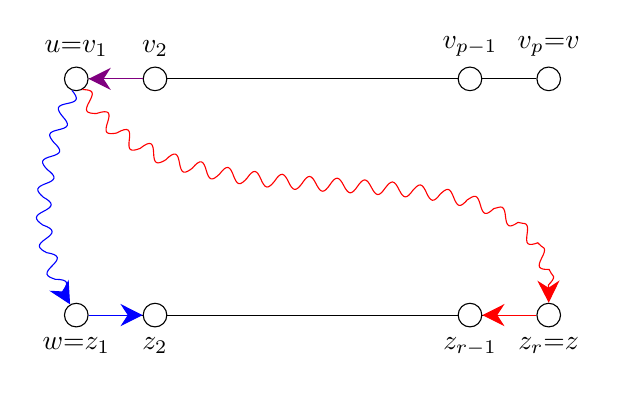
\begin{tikzpicture}
			%%%S_uv
			\node[vert,label=above:$u {=} v_1$] (v1) at (1,0) {};
			\node[vert,label=above:$v_2$] (v2) at (2,0) {};
			\node[vert,label=above:$v_{p-1}$] (vp1) at (6,0) {};
			\node[vert,label=above:$v_p {=} v$] (vp) at (7,0) {};
			\draw (v1) -- (v2) -- (vp1) -- (vp);
			
			%%%% S_wz
			\node[vert,label=below:$w {=} z_1$] (z1) at (1,-3) {};
			\node[vert,label=below:$z_2$] (z2) at (2,-3) {};
			\node[vert,label=below:$z_{r-1}$] (zr1) at (6,-3) {};
			\node[vert,label=below:$z_r {=} z$] (zr) at (7,-3) {};
			\draw (z1) -- (z2) -- (zr1) -- (zr);
			
			
			\draw [violet] (v2) edge[diredge2] (v1);
			
			\draw [blue]%[transform canvas={yshift=0.5mm},thick] 
			(v1) edge[dirwave] [out=250,in=120] (z1) 
			(z1) edge[diredge2] (z2);
			
			
			\draw [red] %[transform canvas={yshift=-0.5mm}] 
			(v1) edge[dirwave] [out=300,in=90] (zr) 
			(zr) edge[diredge2] (zr1);
		\end{tikzpicture}}
	\caption{Example of a guess G-\ref{FPT-guessFTPamongv2z2}, where we guessed the fastest temporal paths of form $v_2 \rightarrow u \leadsto w \rightarrow z_2$ (in blue)
	and $v_2 \rightarrow u \leadsto z \rightarrow z_{r-1}$ (in red).
	\label{fig:FPT-guessG4}}
	\end{subfigure}
	\quad
	\begin{subfigure}[b]{0.48\textwidth}
		\centering
		\resizebox{\linewidth}{!}{
			
			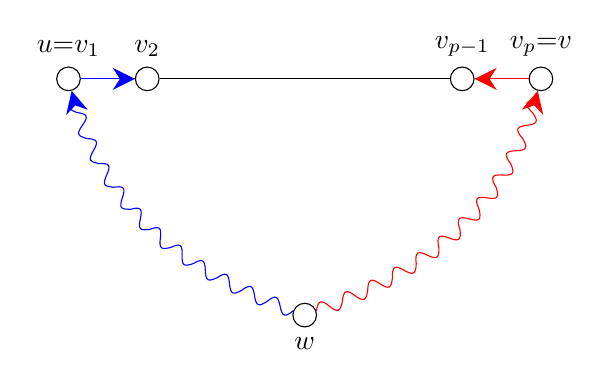
\begin{tikzpicture}
				%%%S_uv
				\node[vert,label=above:$u {=} v_1$] (v1) at (1,0) {};
				\node[vert,label=above:$v_2$] (v2) at (2,0) {};
				\node[vert,label=above:$v_{p-1}$] (vp1) at (6,0) {};
				\node[vert,label=above:$v_p {=} v$] (vp) at (7,0) {};
				\draw (v1) -- (v2) -- (vp1) -- (vp);
				
				%%%% node w
				\node[vert,label=below:$w$] (w) at (4,-3) {};
				
				
				
				\draw [blue]%[transform canvas={yshift=0.5mm},thick] 
				(w) edge[dirwave] [out=160,in=285] (v1) 
				(v1) edge[diredge2] (v2);
				
				\draw [red]%[transform canvas={yshift=0.5mm},thick] 
				(w) edge[dirwave] [out=20,in=255] (vp) 
				(vp) edge[diredge2] (vp1);
				
				
			\end{tikzpicture}}
		\caption{Example of a guess G-\ref{FPT:guess-uToSegmentz2}, where we guessed the fastest temporal paths of form $w \leadsto u \rightarrow v_2$ (in blue) and $w \leadsto v \rightarrow v_{p-1}$ (in red). 
			\label{fig:FPT-guessG5}}
	\end{subfigure}
	
	\begin{subfigure}[b]{0.48\textwidth}
			\centering
			\resizebox{1.2\linewidth}{!}{
				%
				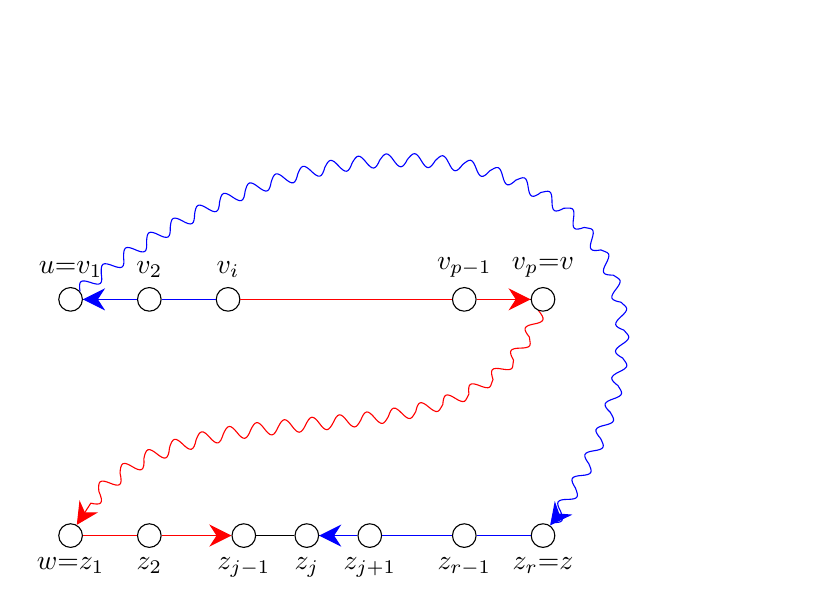
\begin{tikzpicture}[scale=1]
					%%%S_uv
					\node[vert,label=above:$u {=} v_1$] (v1) at (1,0) {};
					\node[vert,label=above:$v_2$] (v2) at (2,0) {};
					\node[vert,label=above:$v_i$] (vi) at (3,0) {};
					\node[vert,label=above:$v_{p-1}$] (vp1) at (6,0) {};
					\node[vert,label=above:$v_p {=} v$] (vp) at (7,0) {};
					\draw (v1) -- (v2) -- (vi) -- (vp1) -- (vp);
					
					%%%% S_wz
					\node[vert,label=below:$w {=} z_1$] (z1) at (1,-3) {};
					\node[vert,label=below:$z_2$] (z2) at (2,-3) {};
					\node[vert,label=below:$z_{j-1}$] (zj-1) at (3.2,-3) {};
					\node[vert,label=below:$z_{j}$] (zj) at (4,-3) {};
					\node[vert,label=below:$z_{j+1}$] (zj+1) at (4.8,-3) {};
					\node[vert,label=below:$z_{r-1}$] (zr1) at (6,-3) {};
					\node[vert,label=below:$z_r {=} z$] (zr) at (7,-3) {};
					\draw (z1) -- (z2) -- (zj-1) -- (zj) -- (zj+1) -- (zr1) -- (zr);
					
					
					
					\draw [blue]%[transform canvas={yshift=0.5mm},thick] 
					(vi) -- (v2) edge[diredge2] (v1) 
					(v1) edge[dirwave] [out=40,in=55,distance=5.2cm] (zr) 
					(zr) --(zr1) -- (zj+1)
					(zj+1) edge[diredge2] (zj);
					
					\draw [red]
					(vi) -- (vp1) edge[diredge2] (vp) 
					(vp) edge[dirwave] [out=250,in=60] (z1) 
					(z1) --(z2)
					(z2) edge[diredge2] (zj-1);
					
					
			\end{tikzpicture}}
			\caption{Example of a guess G-\ref{FPT:guess-splitFromAnotherSegmentAndPaths}, where, for fixed a vertex $v_i \in S_{u,v}$,
				we calculated its corresponding split vertex $z_j \in S_{w,z}$,
				and guessed the fastest paths of form
				$v_i \rightarrow v_{i-1} \rightarrow \cdots \rightarrow u \leadsto z \rightarrow z_{r-1} \cdots \rightarrow z_j$ (in blue) 
				and $v_i \rightarrow v_{i+1} \rightarrow \cdots \rightarrow v \leadsto w \rightarrow z_2 \rightarrow \cdots \rightarrow z_{j-1}$ (in red). 
				\label{fig:FPT-guessG6}}
		\end{subfigure}
	\quad
	\begin{subfigure}[b]{0.48\textwidth}
		\centering
		\resizebox{\linewidth}{!}{
		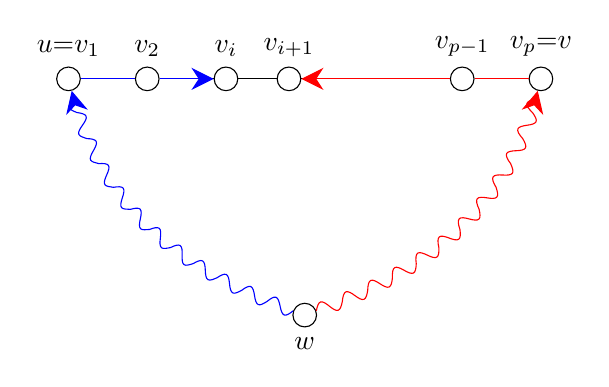
\begin{tikzpicture}
			%%%S_uv
			\node[vert,label=above:$u {=} v_1$] (v1) at (1,0) {};
			\node[vert,label=above:$v_2$] (v2) at (2,0) {};
			\node[vert,label=above:$v_i$] (vi) at (3,0) {};
			\node[vert,label=above:$v_{i+1}$] (vi+1) at (3.8,0) {};
			\node[vert,label=above:$v_{p-1}$] (vp1) at (6,0) {};
			\node[vert,label=above:$v_p {=} v$] (vp) at (7,0) {};
			\draw (v1) -- (v2) -- (vi) -- (vi+1) -- (vp1) -- (vp);
			
			%%%% node w
			\node[vert,label=below:$w$] (w) at (4,-3) {};
			
			
			
			\draw [blue] 
			(w) edge[dirwave] [out=160,in=285] (v1) 
			(v1) -- (v2)
			(v2) edge[diredge2] (vi);
			
			\draw [red]
			(w) edge[dirwave] [out=20,in=255] (vp) 
			(vp) -- (vp1)
			(vp1) edge[diredge2] (vi+1);
			
		\end{tikzpicture}}
	\caption{Example of a guess G-\ref{FPT:guess-splitFromUtoAnotherSegment}, where, for a vertex of interest $w$, 
		we
		calculated its corresponding split vertex $v_i \in S_{u,v}$,
		and guessed the fastest paths of form
		$w \leadsto u \rightarrow v_2 \rightarrow \cdots \rightarrow v_i$  (in blue) 
		and $w \leadsto v \rightarrow v_{p-1} \rightarrow \cdots \rightarrow v_{i+1}$ (in red). 
		\label{fig:FPT-guessG7}}
	\end{subfigure}
\caption{An example of guesses G-4, G-5, G-6 and G-7.}
\end{figure}
%
We create all of the guesses independently.
We start with the first one, that results in $O(k^{k^3})$ different possibilities, then we split each one of these guesses into $O(k^{k^6})$ new ones, that respond to the guessing in the second step, etc.
After creating all of the guesses we end up with exponential in $k$ different cases.
We now create one ILP instance for each case.
From now on we assume that we know exactly the structure of all paths we have guessed and the permutation of all variables.

\subsection{Properties of \deltaExact}

In this section we study the properties of our problem, that then help us creating constraints of our ILP.
Remember, with $G$ we denote our underlying graph of $D$. We want to determine labeling $\lambda$ of each edge of $G$.
We start with an empty labeling of edges and start adding certain values to them.
Note, these values are not (necessarily) numbers. 
In fact at the beginning the values will be determined with respect to each other (\ie as a function of each other).
In our analysis we exploit the following greatly, that is why we state is as an observation.

\begin{observation}\label{obs:FirstLabelAndDuration}
    Let $P$ be the underlying path of a fastest temporal path from $u$ to $v$, where $e_1, e_p \in P$ are its first and last edge, respectively.
    Then, knowing the label $\lambda (e_1)$ of the first edge and the duration $d(P,\lambda)$ of the temporal path $(P,\lambda)$, we can uniquely determine the label $\lambda (e_p)$ of the last edge of $P$.
    Symmetrically, knowing $\lambda(e_p)$ and $d(P)$, we can uniquely determine $\lambda(e_1)$.
\end{observation}
The correctness of the above statement follows directly from \cref{def:temporalPath+Duration}. Since the duration of $(P,\lambda)$ is calculated as the difference of labels of last and first edge plus $1$,
where the label of last edge is considered with some delta periods,
\ie $d(P,\lambda) = p_i \Delta + \lambda(e_p) - \lambda (e_1) + 1$, for some $p_i \geq 0$.
Therefore $d(P,\lambda) \pmod \Delta \equiv  (\lambda(e_p) - \lambda (e_1) + 1) \pmod \Delta$.

In the following we prove that knowing the structure (the underlying path) of a fastest temporal path $P$, from a vertex of interest $u$ to a vertex of interest $v$,
results in determining the labeling of each edge in the fastest temporal path from $u$ to $v$ 
(with the exception of some constant number of edges), with respect to the label of the first edge.
More precisely, if path $P$ from $u$ to $v$ is a segment, then we can determine labels of all edges,
and if $P$ consists of $\ell$ segments, then we can determine the labels of all but $\ell -1$ edges.
For the exact formulation and proofs see \cref{lemma:FPT-uv-Labelalledges,lemma:FPT-uv-LabelAlmostalledges}.

\begin{lemma}\label{lemma:FPT-uv-Labelalledges}
    Let $u, v \in U$ be two arbitrary vertices of interest and suppose that $P = (u=v_1,v_2, \dots, v_p = v)$, where $p \geq 2$, 
    is a $u,v$ path in $G'$, which is also the underlying path of a fastest temporal path from $u$ to $v$.
    Moreover suppose also that $P$ is a segment.
    %Suppose also that no other vertex from $P$ is a vertex of interest, \ie $P \setminus \{u,v\} \cap U = \emptyset$.
    We can determine the labeling $\lambda$ of every edge in $P$ with respect to the label $\lambda(uv_2)$ of the first edge.
    %such that the labeling $\lambda$ respects $D'$.
\end{lemma}

\begin{proof}
We claim that $u$ reaches all of the vertices in $P$ the fastest, when traveling along $P$ (\ie by using a subpath of $P$).
To prove this suppose for the contradiction that there is a vertex $v_i \in P \setminus \{u,v\}$, that is reached from $v$ on a path different than $P_i = (u, v_2, v_3, \dots, v_i)$.
Since the only vertices of interest of $P$ are $u$ and $v$, it follows that all other vertices on $P$ are of degree $2$. 
Then the only way to reach $v_i$ from $u$, that differs from $P$, would be to go from $u$ to $v$ using a different path $P_2$,
and then go from $v$ to $v_{p-1}, v_{p-2}, \dots, v_i$.
But since $P$ is the fastest temporal path from $u$ to $v$, we get that $d(P_2) \geq d(P)$ and $d(P_2 \cup (v,v_{p-1}, \dots, v_i)) > d(P) > d(P_i)$.

Now to label $P$ we use the fact that the fastest temporal path from $u$ to any $v_i \in P$ is a subpath of $P$, 
therefore we can label each edge using \cref{obs:FirstLabelAndDuration},
where the duration from $u$ to $v_i$ equals to $D_{u,v_i}$ and 
we set the first label of $P$ to be a constant $c_{uv}$.
This gives us a unique label for each edge of $P$, that depends on the value $c_{uv}$.
\end{proof}

\begin{lemma}\label{lemma:FPT-uv-LabelAlmostalledges}
    Let $u, v \in U$ be two arbitrary vertices of interest and suppose that $P = (u=v_1, v_2, \dots, v_p = v)$, where $p \geq 2$, 
    is a $u,v$ path in $G'$, which is also the underlying path of a fastest temporal path from $u$ to $v$.
    Let $\ell_{u,v} \geq 1$ be the number of vertices of interest in $P$ different to $u,v$, namely $\ell_{u,v} = | v_i \in \{P \setminus \{u,v \} \} \cap U |$.
    We can determine the labeling $\lambda$ of all but $\ell_{u,v}$ edges of $P$, with respect to the label $\lambda(uv_2)$ of the first edge,
    such that the labeling $\lambda$ respects the values from $D$.
    Moreover, for the labels of edges that cannot be determined precisely, we can get some extra restrictions.
\end{lemma}

\begin{proof}
We denote with $v_i \in U$ a vertex of interest in $P \setminus \{u,v\}$.
There are two options, either $v_i$ is reached from $u$ using the subpath $P_i = (u, v_2, v_3, \dots, v_i)$ of $P$,
or there exists a fastest temporal path $P' = (u, w_2, w_3, \dots, w_{p'} = v_i)$, for which $P \cap P' = \{u, v_i\}$.
If the temporal path from $u$ to $v_i$ is a subpath of $P$, then we determine the labeling of $P$ using \cref{lemma:FPT-uv-Labelalledges}.
So we can suppose that the fastest temporal path from $u$ to $v_i$ is of form $P'$.
\todo[inline]{George proved it. Also: add notation that is used in the proof to the beginning of the section, namely: $d(u,v,P)$ is the duration of the temporal path from $u$ to $v$ that traverses the edges of $P$.}
\end{proof}

%Observe also the following.

\begin{lemma}\label{lemma:FPT-unlabeldPaths-01}
    Suppose that
    $S_{u,v}, S_{w,z}$ are two segments with $ v_i \in S_{u,v}$ and $z_j \in S_{w,z}$,
    where $z_j$ is a split vertex of $v_i$ in the segment $S_{w,z}$.
    W.l.o.g. suppose that the fastest temporal path from $v_i$ to $z_j$ travels through vertices $u$ and $w$.
    Then the fastest temporal path from $v_i$ to any other vertex of $S_{w,z}$, that is closer to $w$,
    travels through the same two vertices $u$ and $w$.
    Similarly it holds for the cases when the fastest temporal path travels through $w,v$ or $z,u$ or $z,v$.
\end{lemma}
\begin{proof}
    Let $z_\ell$ be a vertex of $S_{w,z}$, that is closer to $w$ than $z$ in the segment.
    Let us denote with $P_{v_i,z_j}$ the underlying path of the fastest temporal path from $v_i$ to $z_j$.
    Denote with $P_{v_i,z_j}^\ell$
    the subpath of the fastest temporal path from $v_i$ to $z_j$, that terminates in $z_\ell$.
    We want to show that $P_{v_i,z_j}^\ell$ is an underlying path of a fastest temporal path from $v_i$ to $z_j$.
    Let us observe the following possibilities.
    \\
    First, suppose for the contradiction, that the fastest temporal path from $v_i$ to $z_\ell$ travels through vertices $u$ and $z$.
    Denote this path as $P^1_{v_i,z_\ell}$.
    Then it follows that $d(P^1_{v_i,z_\ell}, \lambda) \leq d(P_{v_i,z_j}^\ell,\lambda)$, which would imply that
    the duration of the temporal path from $v_i$ to $z_j$ using the subpath of $P^1_{v_i,z_\ell}$, would be strictly smaller than the duration of $(P_{v_i,z_j},\lambda)$, which cannot be possible.
    \\
    Second, suppose that the fastest temporal path from $v_i$ to $z_\ell$ travels through vertices $v$ and $w$.
    Denote this path as $P^2_{v_i,z_\ell}$.
    Note that $P_{v_i,z_j}^\ell$ and $P^2_{v_i,z_\ell}$ intersect on a segment $S_{w,z}$ from the vertex $w$ to $z_\ell$.
    Therefore since
    $d(P^2_{v_i,z_\ell}, \lambda) \leq d(P_{v_i,z_j}^\ell,\lambda)$,
    and since there is unique way to
    extend the path $P^2_{v_i,z_\ell}$ from $z_\ell$ to $z_j$, denote the extended path as $P^j_{v_i,z_\ell}$,
    we get that $d(P^j_{v_i,z_\ell}, \lambda) \leq $$(P_{v_i,z_j},\lambda)$.
    Which implies that $d(P^j_{v_i,z_\ell}, \lambda) = d(P_{v_i,z_j}, \lambda)$.
    Now using the similar argument it follows that $d(P_{v_i,z_j}^\ell, \lambda) = d(P^2_{v_i,z_\ell}, \lambda)$,
    therefore $P_{v_i,z_j}^\ell$ is also a fastest temporal path from $v_i$ to $z_j$.
    \\
    Third, suppose that the fastest temporal path from $v_i$ to $z_\ell$ travels through vertices $v$ and $z$.
    Denote this path as $P^3_{v_i,z_\ell}$.
    Then the duration of the temporal path from $v_i$ to $z_j$ using the subpath of $P^3_{v_i,z_\ell}$, would be strictly smaller than the duration of $(P_{v_i,z_j},\lambda)$, which cannot be possible.
\end{proof}

\begin{lemma}\label{lemma:FPT-noUndeterminedEdgeInSegment}
Let $S_{u,v}$ be a segment in $G$ of length at least $5$,
\ie $S_{u,v}= (u=v_1,v_2, \dots, v_p = v)$, where $p > 5$.
It cannot happen that an inner edge $f = v_i v_{i+1}$ from $S_{u,v} \setminus \{u,v\}$,
is not a part of any fastest temporal path, of length at least $2$, among vertices in $S_{u,v}$,
\ie there has to be a pair $v_j, v_{j'} \in S_{u,v}$ \st the fastest temporal path from $v_j$ to $v_{j'}$ passes through edge $f$.
In the case when $p = 5$ all temporal paths of length $2$ avoid $f$ if and only if $f$ has the same label as both of the edges incident to it.
\end{lemma}

\begin{proof}
    For an easier understanding and better readability we present the proof for $S_{u,v}$ of fixed length $5$.
    The case, when $S_{u,v}$ is longer easily follows from presented results.

    Let $S_{u,v} = (u=v_1,v_2, v_3, v_4, v_5, v_6=v)$.
    We distinguish two cases, first when $f = v_2v_3$ (note that the case with $f = v_4v_5$ is symmetrical),
    and the second when  $f = v_3v_4$.
    Throughout the proof we denote with $t_i$ the label of edge $v_i v_{i+1}$.
    Suppose for the contradiction, that none of the fastest temporal paths among vertices of $S_{u,v}$ traverses the edge $f$.

    Case 1,  $f = v_2v_3$.
    Let us observe the case of fastest temporal paths among $v_{1}$ and $v_{3}$.
    Denote with $Q = (v_{1}, v_2, v_3)$ and with $P' = (v_3,v_4,v_5,v_6)$.
    From our proposition it follows that
    \begin{itemize}
        \item the fastest temporal path $P ^ +$ from $v_1$ to $v_3$ 
    is of the following form 
    $P^+ = v_{1}  \leadsto v_6 \rightarrow v_5 \rightarrow v_4 \rightarrow v_3$,
    and
        \item the fastest temporal path $P ^ -$ from $v_{3}$ to $v_{1}$ 
    is of the following form 
    $P^- = v_{3} \rightarrow v_{4} \rightarrow v_5 \rightarrow v_6 \leadsto v_1$.
    \end{itemize}
    It follows that 
    $
    d(v_{1}, v_{3}, P^+) \leq d(v_{1}, v_{3}, Q),
    $
    and
    $
    d(v_{1}, v_{3}, P^-) \leq d(v_{1}, v_{3}, Q)
    $.
    Let 
    Note that $d(v_{1}, v_{3}, P^+) \geq 1 + d(v_6,v_3,P')$,
    and by the definition $d(v_6,v_3,P') = 1 + (t_4 - t_5)_\Delta + (t_3 - t_4)_\Delta$,
    where $(t_i - t_j)_\Delta$ denotes the difference of two consecutive labels $t_i, t_j$ modulo $\Delta$.
    Similarly holds for $d(v_{1}, v_{3}, P^+)$.
    Summing now both of the above equations we get
    \begin{equation}
    \begin{split} \label{eq:FPT-prf-fUnlabeled}
        d(v_{1}, v_{3}, P^+) + d(v_{3}, v_{1}, P^-) &\leq 
        d(v_{1}, v_{3}, Q) + d(v_{3}, v_{1}, Q) \\
        %
        1 + d(v_6,v_3,P') + 1 + d(v_3,v_6,P') &\leq d(v_{1}, v_{3}, Q) + d(v_{3}, v_{1}, Q) \\
        %
        2 + 
        1 + (t_4 - t_5)_\Delta + (t_3 - t_4)_\Delta +
        1 + (t_4 - t_3)_\Delta + (t_5 - t_4)_\Delta 
        &\leq 
        1 + (t_2 - t_1)_\Delta + 
        1 + (t_1 - t_2)_\Delta\\
        %
        (t_4 - t_5)_\Delta + (t_5 - t_4)_\Delta +
        (t_4 - t_3)_\Delta + (t_3 - t_4)_\Delta  + 2 
        &\leq 
        (t_2 - t_1)_\Delta + (t_1 - t_2)_\Delta.
    \end{split}
    \end{equation}
    Note that if $t_i \neq t_j$ we get that 
    the sum
    $(t_i - t_j)_\Delta + (t_j - t_i)_\Delta$ equals exactly $\Delta$,
    and if $t_i = t_j$ the sum equals $2\Delta$.
    This follows from the definition of travel delays at vertices (see \cref{obs:travel-delays-both-directions}).
    Therefore we get from \cref{eq:FPT-prf-fUnlabeled}, 
    that the right part is at most $2 \Delta$, while the left part is at least $2 \Delta + 1$,
    for any relation of labels $t_1,t_2, \dots, t_5$,
    which is a contradiction.

    Case 2,  $f = v_3v_4$.
    Here we consider the fastest paths among vertices $v_{2}$ and $v_{4}$.
    By similar arguments as above we get
    \begin{align*}
        (t_5 - t_1)_\Delta + (t_4 - t_5)_\Delta + (t_5 - t_4)_\Delta + (t_1 - t_5)_\Delta + 2 \leq (t_3 - t_2)_\Delta + (t_2 - t_3)_\Delta,
    \end{align*}
    which is impossible.
    
    In the case when $S_{u,v}$ is longer, we would get even bigger number on the left hand side of \cref{eq:FPT-prf-fUnlabeled}, 
    so we conclude that in all of the above cases, it cannot happen that all fastest paths of length $2$, among vertices in $S{_u,v}$, avoid an edge $f$.

    Let us observe now the case when $S_{u,v} = (u=v_1,v_2, v_3, v_4, v_5=v)$ is of length $4$.
    Let $f = v_2 v_3$ (the case with $f = v_3 v_4$ is symmetrical).
    Suppose that the fastest temporal paths among $v_1$ and $v_3$ do not use the edge $f$.
    We denote with $R^+$ the fastest path from $v_1$ to $v_3$, 
    which is of form $u \leadsto v \rightarrow v_4 \rightarrow v_3$,
    and similarly 
    with $R^-$ the fastest path from $v_3$ to $v_1$, which is
    of form $v_3 \rightarrow v_4 \rightarrow v \leadsto u$.
    We denote with $R' = (v_3, v_4, v_5)$ and with $S = (v_1,v_2,v_3)$.
    Again we get the following.
    \begin{equation}
    \begin{split}
        d(v_{1}, v_{3}, R^+) + d(v_{3}, v_{1}, R^-) &\leq 
        d(v_{1}, v_{3}, S) + d(v_{3}, v_{1}, S) \\
        %
        1 + d(v_5,v_3,R') + 1 + d(v_3,v_5,R') &\leq d(v_{1}, v_{3}, S) + d(v_{3}, v_{1}, S) \\
        %
        (t_3 - t_4)_\Delta + (t_4 - t_3)_\Delta + 2 
        &\leq 
        (t_2 - t_1)_\Delta + (t_1 - t_2)_\Delta.        
    \end{split}
    \end{equation}
    The only case when the equation has a valid solution is when $t_1 = t_2$ and $t_3 \neq t_4$,
    since in this case the left hands side evaluates to $\Delta + 2$, while the right side evaluates to $2 \Delta$.\\
    Repeating the analysis for the fastest paths among $v_2$ and $v_4$,
    we get that the only valid solution is when $t_2 = t_3$ and $t_1 \neq t_4$.
    Altogether, we get that $f$ is not in a fastest path of length $2$ in $S_{u,v}$ if and only if the label of edge $f$ is the same as the labels on the edges incident to it, while the last remaining edge has a different label.
\end{proof}

\subsection{Adding constraints and variables to the ILP}
First case we observe is the case when we want to determine the labels on fastest temporal paths among vertices of interest.
We proceed in the following way.
Let $u,v \in U$ be two vertices of interest and let $P_{u,v}$ be the fastest temporal path from $u$ to $v$.
If $P_{u,v}$ is a segment we determine all the labels of edges of $P$, with respect to the label of the first edge (see \cref{lemma:FPT-uv-Labelalledges}).
%Note that since we determined labels of all edges, with respect to the first edge, we also know the exact values of waiting times at each inner vertex of $P_{u,v}$, when traversing the path.
In the case when $P_{u,v}$ is a sequence of $\ell$ segments, we determine all but $\ell - 1$ labels of edges of $P_{u,v}$, with respect to the label of the first edge (see \cref{lemma:FPT-uv-LabelAlmostalledges}). \todo{Change/explain what ``with respect to first label'' means}
%In both cases we introduce the equality constraint for $P_{u,v}$ (as in \cref{eq:FPT-equalityConstraint}).
%Since there are $\ell - 1$ edge labels that are not determined with respect to the label of the first edge, may be some  TODO from above??

After finishing the previous step for all pairs of vertices in $U$,
the edges of fastest temporal paths from $u$ to $v$, where $u,v \in U$, are determined with respect to the label of the first edge of each path.
Let us call these edges \emph{determined edges}, and the edges that were not determined with the respect to some other edge label up to now the \emph{not yet determined} edges.
If the fastest temporal path among two vertices $u,v \in U$ is just an edge $e$, then we treat it as being determined, since it gets assigned a label $\lambda(e)$ with respect to itself.
Note that the not yet determined edges are exactly the ones that are not a part of any fastest temporal path.
Let us first observe some properties of such edges.

\begin{lemma}
    Not yet determined edges form disjoint segments in $G'$, where each segment starts and ends in some vertex of interest, 
    \ie for every not yet determined path $P$ there exist $u,v \in U$, such that $P = (u, v_1, v_2, \dots, v_p=v)$, where $p \geq 0$ and $v_1,v_2,\dots,v_{p-1} \in V(G') \setminus U$.
\end{lemma}
\begin{proof}
    We prove this claim in two steps.
    First we prove that all inner vertices of $P$, \ie vertices $v_i \in  S \setminus \{u,v\}$ are of degree exactly $2$ and are not vertices of interest. 
    They are of degree at least $2$ since they are on a path $P$ and are incident to two not yet determined edges in  $P$.
    They are of degree at most $2$ as if they were of a higher degree they would be vertices of interest and in this case we could split $P$ into shorter segments (subpaths).
    
    Second, suppose that $P$ does not start in a vertex of interest, therefore $u \notin U$. As $u$ is the starting vertex of the not yet determined path $P$, there must exist a vertex of interest $u'$ such that a path between $u$ and $u'$ is labeled.
    Since $u$ is not a vertex of interest, the only reason to label edges between $u'$ and $u$ would be if they were a part of some fastest temporal path among two vertices of interest and $u$ would be an inner vertex on that path.
    Therefore $u$ would have to be incident to two labeled edges (that are part of some fastest temporal path) and one not yet determined edge, but in this case the degree of $u$ would be at least $3$ and therefore $u$ would be a vertex of interest.

    From all of the above, it follows that $P$ is a not yet determined segment in $G'$.
\end{proof}

\begin{lemma}
    After determining the labels of fastest temporal paths between all pairs of vertices of interest,
    there can be at most one not yet determined segment among each pair of them.
    %among any pair of vertices of interest $u,v \in U$ there can be at most one undetermined segment $S = (u, v_1, v_2, \dots, v_p, v)$, where $p \geq 0$ and $v_1,v_2,\dots,v_p \in V(G') \setminus U$.
\end{lemma}
\begin{proof}
   Suppose for the contradiction that after determining the labels of all fastest temporal paths between vertices of interest,
   there are two not yet determined segments among $u,v \in U$.
   Denote them with $S_{u,v}$ and $S'_{u,v}$. 
   Then $C = S_{u,v} \cup S_{u,v}'$ forms a cycle in $G'$. Since $G'$ admits no loops, the cycle $C$ is of length at least $3$.
   Since $C$ is a cycle, at least one of its edges $e \in E(C)$ has to be in the feedback edge set $F$, and therefore, by the definition of vertices of interest $U$, 
   both endpoints of $e$ have to be in $U$.
   If $e = uv$ then there are only two vertices of interest in $C$, but the label of edge $e$ is determined.
   And if $e \neq uv$ then there are at least $3$ vertices of interest in $C$.
   So $S_{u,v}$ and $S_{u,v}'$ cannot be both fully not yet determined.
\end{proof}
From the above it follows that
after we finish determining the labels for all fastest temporal paths among vertices of interest,
there is at most one fully determined segment among two vertices of interest and at most one undetermined segment.
Therefore the following holds.
\begin{corollary}\label{obs:FPT-k2segments}
    There are at most $O(k^2)$ segments in $G'$.
\end{corollary}


Now we want to relate the not yet determined segments with the determined ones.
Let $S_{u,v}$ and $S_{w,z}$ be two segments.
At the beginning we have guessed the fastest path from $v_i$ to all vertices in $S_{w,z}$ (see guess G-\ref{FPT:guess-splitFromAnotherSegmentAndPaths}).
We did this by determining which vertices $z_j, z_{j+1}$ in $S_{w,z}$ are furthest away from $v_i$
(remember we can have the case when $z_j = z_{j+1}$),
and then we guessed how the path from $v_i$ leaves the segment $S_{u,v}$ (\ie either through the vertex $u$ or $v$),
and then how it reaches $z_j$ (in the case when $z_j \neq z_{j+1}$ there is a unique way,
when $z_j = z_{j+1}$ we determined which of the vertices $w$ or $z$ is on the fastest path).
W.l.o.g. assume that we have guessed that the fastest path from $v_i$ to $z_j$
passes through $w$ and $z_{j-1}$.
Then the fastest temporal path from $v_i$ to $z_{j+1}$ passes through $z$.
And all fastest temporal paths from $v_i$ to any $z_{j'} \in S_{w,z}$
use all of the edges in $S_{w,z}$ with the exception of the edge $z_j z_{j+1}$.
Using this information and \cref{obs:FirstLabelAndDuration}, we can determine the labels on all edges, with respect to the first or last label from the segment $S_{u,v}$,
with the exception of the edge $z_j z_{j+1}$.
Therefore, all edges of $S_{w,z}$ but $z_j z_{j+1}$ become determined.
Since we repeat that procedure for all pairs of segments,
we get that for a fixed segment $S_{w,z}$ we end up with a not yet determined edge $z_j z_{j+1}$
if and only if, this is a not yet determined edge in relation to every other segment $S_{u,v}$ and its fixed vertex $v_i$.
%
We repeat this procedure for all pairs of segments.
Each specific calculation takes linear time, since there are $O(k^2)$ segments, this calculation takes $O(k^4)$ time.
At this point
the edges of every segment are fully determined, 
with the exception of at most three edges per segment (the first and last edge and potentially one extra somewhere in the segment).
We will now relate also these edges.
More precisely,
let $S_{u,v} = (u=v_1, v_2, \dots, v_p=v)$ be a segment with three not yet determined edges,
and let $e_i =v_iv_{i+1}$ denote an edge of $S_{u,v}$.
From the above procedure (when we were determining labels of edges of segments with each other) 
we conclude that all of the edges $e_i$ of $S_{u,v}$ are in the following relation.
There are some edges $e_1, e_2, \dots e_{i-1}$, whose label is determined with respect to the label $\lambda(e_1)$,
we have an edge $f = e_i = v_i v_{i+1}$ which is not yet determined,
and then there follow the edges
$e_{i+1}, e_{i+2}, \dots, e_{p-1}$, whose labels are determined with respect to the $\lambda(e_{p-1})$.
We want to now determine all of the edges in such segment $S_{u,v}$ with respect to just one edge (either the first or the last one).
For this we use the fact that at least one of the temporal paths among vertices in $S_{u,v}$ has to pass through $f$, when $S_{u,v}$ has at least $5$ edges (see~\cref{lemma:FPT-noUndeterminedEdgeInSegment}).
We proceed as follows.
\begin{enumerate}[G-1.]
    \setcounter{enumi}{\value{guesscounter}}
    \item \label{FPT-guessFTPinSegmentTgroughEdge}
    For every segment $S_{u,v} = (u=v_1, v_2, \dots, v_p=v)$  with a not yet determined edge $v_i v_{i+1} = f \in S_{u,v}$,
    we guess which of the following fastest temporal paths pass through the edge $f$,
    one of the fastest paths between $v_{i-1}$ and $v_{i+1}$ (either from $v_{i-1}$ to $v_{i+1}$, or vice versa), 
    and 
    one of the fastest paths between $v_{i}$ and $v_{i+2}$.
    We create $4$ guesses for each such segments, therefore we create $O(k^2)$ new guesses in total, as there are at most $O(k^2)$ segments.
    % counter for guesses continues
    \setcounter{guesscounter}{\value{enumi}}
\end{enumerate}
Once we know which two fastest temporal paths pass through $f$, 
we can determine the label of edge $f$ 
with respect to the first edge of the segment (when considering the fastest temporal path between $v_{i-1}$ and $v_{i+1}$),
and with respect to the last edge of the segment (when considering the fastest temporal path between $v_{i}$ and $v_{i+2}$).
Both these steps together determine all of the labels of $S_{u,v}$ with respect to just one label.
Note, from \cref{lemma:FPT-noUndeterminedEdgeInSegment} it follows that the above procedure holds only for segments with at least $5$ edges.
In the case when segment has $4$ edges, it can happen that the fastest temporal paths from above, do not traverse $f$. But in this case we get that $3$ labels of edges in the segment have to be the same, while one is different,
which results in a segment with two not yet determined edges.
In the case when the segment $S_{u,v}$ has just three, two or one edge, this procedure does not improve anything,
therefore these segments remain with three, two or one not yet determined edges, respectively.
From now on we refer to segments of length less than $4$.

At this point $G$ is a graph, where each edge $e$ has a value for its label $\lambda(e)$
that depends on (\ie is a function of) some other label $\lambda(f)$ of edge $f$,
or it depends on no other label.
We now describe how we create variables and start building our ILP instances. 
For every edge $e$ in $G'$ that is incident to a vertex of interest we create a variable $x_e$ that can have values from $ \{1, 2, \dots, \Delta\}$.
Besides that we create one variable for each edge that is still not yet determined on a segment.
Since each vertex of interest is incident to at most $k$ edges, and each segment has at most one extra not yet determined edge, we create $O(k^2)$ variables.
At the end we create our final guess
\begin{enumerate}[G-1.]
% counter for guesses continues
\setcounter{enumi}{\value{guesscounter}}
%%
    \item \label{FPT:guessallPermutations}
We guess the permutation of all $O(k^2)$ variables,
together with the relation of each variable to the labels of edges incident to these not yet determined edges.
Namely, for an edge $e$ that is not yet determined, we set its value to $x_e$ and check labels of all of its neighbors,
which are determined by some other label,
and variables of the not yet determined neighbors,
and guess if $x_e$ is smaller, equal or bigger than the labels of the edges of its neighbors.
So, for any two variables $x_e$ and $x_f$, we know if $x_e < x_f$ or $x_e = x_f$, or $x_e > x_f$,
and for any neighboring edge $g$ of $e$ we know if $x_e < \lambda(g)$ or 
$x_e = \lambda(g)$, or $x_e > \lambda(g)$.
This results in $O(k^2 !) = O(k^{2k^2}) = O(k^{k^3})$ guesses
and consequently
each of the ILP instances we created up to now is further split into $O(k^{k^3})$ new ones.
\end{enumerate}

We proceed with adding constraints to each of our ILP instances.
First we add all constraints for the labels of edges that we have determined up to now.
We then continue to iterate through all pairs of vertices and start adding equality (resp.~inequality) constraints for the fastest (resp.~non-fastest) temporal paths among them.

We now describe how we add constraints to a path. Whenever we say that a duration of a path gives an equality or inequality constraint, we mean the following.
Let $P=(u=v_1,v_2, \dots, v_p = v)$ be the underlying path of a fastest temporal path from $u$ to $v$,
and let $Q = (u=z_1,z_2, \dots, z_r = v)$ be the underlying path of another temporal path from $u$ to $v$.
Then we know that $d(P,\lambda) = D_{u,v}$ and $d(Q, \lambda) \geq D_{u,v}$.
Using \cref{obs:durationPwithWaitingTimes}
we create an \emph{equality constraint} for $P$
of the form 
\begin{equation}\label{eq:FPT-equalityConstraint}
    D_{u,v} = \sum _ {i=2} ^ {p-1} (\lambda (v_{i}v_{i+1}) - \lambda (v_{i-1}v_i))_\Delta + 1,
\end{equation}
and an \emph{inequality constraint} for $Q$ 
\begin{equation}\label{eq:FPT-inequalityConstraint}
    D_{u,v} \leq \sum _ {i=2} ^ {r-1} (\lambda (z_{i}z_{i+1}) - \lambda (z_{i-1}z_i))_\Delta + 1.
\end{equation}
In both cases we implicitly assume that if the difference of $(\lambda (z_{i}z_{i+1}) - \lambda (z_{i-1}z_i))$ is negative, for some $i$, we add the value $\Delta$ to it (\ie we consider the difference modulo $\Delta$), therefore we have the sign $\Delta$ around the brackets.
Note that we know if the difference of two consecutive labels is positive or negative. 
In the case when two consecutive labels are determined with respect to the same label $\lambda(e)$ the difference among them is easy to determine,
if one or both consecutive labels are not yet determined 
then we have guessed in what kind of relation they are (see guess G-~\ref{FPT:guessallPermutations}).
Therefore we know when $\Delta$ has to be added, which implies that \cref{eq:FPT-equalityConstraint,eq:FPT-inequalityConstraint} are calculated correctly for all paths.

We iterate through all pairs of vertices $x,y$ and make sure that the fastest temporal path from $x$ to $y$ produces the equality constrain \cref{eq:FPT-equalityConstraint},
and all other temporal paths from $x$ to $y$ produce the inequality constraint \cref{eq:FPT-inequalityConstraint}.
For each pair we argue how we determine these paths.

\subsubsection*{\boldmath Fastest paths among $u,v$ where $u \in U$ and $v \in V$}
First we consider the case when $u,v$ are two vertices of interest.
This was the case that we partially studied at the beginning of the algorithm, that helped us determine certain labels of the graph.
We now iterate again through all fastest temporal paths from $u$ to $v$ and introduce an equality constraint for them.
We then continue 
through all of the paths from $u$ to $v$, and for every one, that is not the underlying path of a fastest temporal path, we add the inequality constraint.
There are $O(k^k)$ possible paths from $u$ to $v$ in $G'$, therefore in this step we introduce $O(k^{k^3})$ constraints.

\subsubsection*{\boldmath Fastest paths among $u,x$ where $u \in U$ and $x \in V(G') \setminus U$}
Next we continue with the case of the fastest path from $u$ to $x$, where $u \in U$ and $x \in V(G') \setminus U$.
From the guesses G-\ref{FPT:guess-uToSegmentz2} and G-\ref{FPT:guess-splitFromUtoAnotherSegment} it follows that we know the fastest temporal paths from $u$ to all vertices in a segment $S_{w,v}$.
In this case we create the equality constraint for the fastest path and
iterate through all other paths, for which we introduce the inequality constraints.
There are $O(k^k)$ possible paths of $u \leadsto w$ (resp.~$u \leadsto v$),
and a unique way how to extend those paths from $w$ (resp.~$v$) to reach $x$ in $S_{w,v}$.
Therefore we add $O(k^k)$ inequality constraints.

%%%%%%
%%%%%% below was done before we had the Guess 7, now we see this case follows easily from it.
\begin{comment}
    
We have three possibilities:
\begin{enumerate}[(i)]
    \item Vertex $x$ is on a segment $S_{u,v}=(u,v_1,v_2,\dots,v_{p-1},v_p = v)$. 
    If $x$ is on a fastest path from $u$ to some other vertex $w \in U$, then we know that the fastest path from $u$ to $x$ is a subpath of the segment $S_{u,v}$.
    We introduce the equality constraint for it.
    We iterate through all possible paths of form $u \leadsto v \rightarrow v_{p-1} \rightarrow \dots \rightarrow x$ and introduce inequaity constraints for them.
    Since there are $O(k^k)$ possible paths from $u$ to $v$, we create $O(k^k)$ inequality constraints.
    
    Suppose now that the segment $S_{u,v}$ is not a part of a fastest path from $u$ to some other vertex $w \in U$.
    Denote with $Q$ the fastest temporal path of form $u \leadsto v \rightarrow v_{p-1}$ (which we know from guess~G-\ref{FPT-guessFTPamongv2z2}).
    We find the vertices $v_i, v_{i'} \in S_{u,v}$ that are on the furthest distance from $u$.
    Note that these two vertices are either neighbors, or the same vertex, \ie $i' \in \{i, i+1\}$.
    Then we know that the fastest temporal paths from $u$ to $v_1, v_2, \dots, v_{i-1}$ travel along $S_{u,v}$,
    and the fastest temporal paths from $u$ to $v_{p-1}, v_{p-2}, \dots, v_{i+1} $ travel along $Q$.
    Therefore we can uniquely determine the fastest temporal path from $u$ to $x$.
    We introduce the equality constraint for these fastest temporal paths, and iterate through all other paths,
    for which we introduce the inequality constraints.
    Note that to find all other paths we need to find all $u \leadsto v$ paths, that we then uniquely extend to $x$.
    Therefore we introduce $O(k^k)$ inequality constraints.
    \item Vertex $x$ is on a fastest temporal path from $u$ to some other vertex of interest $v$, 
    but it does not lie on the segment $S_{u,v}$.
    Suppose that $x$ lies on a segment $S_{w,z}$.
    Then by \cref{lemma:FPT-uv-LabelAlmostalledges} we know that the fastest temporal path from $u$ to $x$ is a subpath of the fastest temporal path from $u$ to $v$.
    This results in adding the equality constraint for this fastest temporal path.
    We now have to iterate through all others temporal paths from $u$ to $x$ and add the inequality constraints.
    To reach $x$ from $u$, we have to first travel from $u$ to $w$ (resp.~$z$), and then travel through $S_{u,w}$ to $x$.
    There are $O(k^k)$ different paths to reach $w$ (resp.~$z$), which are then uniquely extended to $x$.
    Therefore we add $O(k^k)$ inequality constraints for all these paths.
    
    \item \label{item:FPT-uToxcase2}
    Vertex $x$ is not on a fastest temporal path from $u$ to any $v \in U$.
    Suppose that $x$ lies on a segment $S_{w,z} = (w=z_1,z_3, \dots, z_r = z)$.
    Since we the fastest paths $Q^+$ of form $u \leadsto w \rightarrow z_2$ and 
    $Q^-$ of form $u \leadsto z \rightarrow z_{r-1}$ Denote with $Q$ the fastest temporal path of form $u \leadsto v \rightarrow v_{p-1}$ (see guess~G-\ref{FPT-guessFTPamongv2z2}),
    we have to only determine how we reach vertex $x$ from the segment (\ie will the fastest path go through $w$ or through $z$).
    This is done,
    by checking the distances from $u$ to $z_i$, for $z_i \in S_{w,z} \setminus \{w,z\}$,
    and determining the split vertex $z_j$ from $u$ on the segment $S_{w,z}$ (\ie vertex $z_i$ in $S_{w,z}$ that has biggest value $D_{u,z_i}$).
    For all vertices $z_i \neq z_j$, we know which part of the segment is used to reach it.
    Namely, if $z_i$ is closer to $w$ than $z_j$ in $S_{w,z}$ we first use the path $Q^+$, that is then uniquely extended to reach $z_i$,
    and similarly 
    if $z_i$ is closer to $z$ than $z_j$ in $S_{w,z}$
    we first use the path $Q^+$, that is then uniquely extended to reach $z_i$.
    We set this path as the fastest temporal path, that must satisfy the equalities and for all other temporal paths
    (\ie paths of form $u \leadsto z \rightarrow z_{r-1} \rightarrow \cdots \rightarrow x$, and paths of form $u \leadsto w \rightarrow z_2 \rightarrow \cdots \rightarrow x$),
    we add the inequalities constraints.
    If $x = w^*$, we have two possibilities, 
    
    we check the values of each one and set the minimum of them, to equal the $D_{u,x}$, 
    if this is even possible, if one is too small we immediately reject.
    Note, we know the durations of fastest temporal paths from $u$ to $z_2$ and $z_{r-1}$. We also know all the labels of the edges of $S_{w,z}$, with respect to each other,
    with the exception of at most one inner edge.
    Therefore we can completely calculate the duration from $u$ to $x=w^*$ coming from one side (\ie either from $w$ or $z$).
    Suppose that the value of the duration of the fastest path from $u$ to $w^*$, through $w$ is
    smaller than $D_{u,x}$, then we reject and stop the calculation.
    If the value equals $D_{u,x}$ we have determined the fastest temporal path and we use it to create equality constraints, while we use the other path, through $z$, to create an inequality constraint.
    If the value is bigger than $D_{u,x}$, we create an inequality constraint for this path and create an equality constraint for the path through $z$.
    We calculate also all other possible paths from $u$ to $x$ and create inequalities for all of them.
    These paths are exactly all the paths from $u$ to $w$ (resp.~$z$), from where we uniquely continue to $x$ through $S_{w,z}$.
    There are $O(k^{k})$ different paths from $u$ to $w$ (resp.~$z$), therefore we add
    $O(k^k)$ inequality constraints for all these paths, for a fixed $u$ and $x$.   
\end{enumerate} 
\end{comment}

Now we proceed with the case of determining the fastest path from $x$ to $u$, where $x \in V(G') \setminus U$ and $u \in U$.
%We use the similar approach as in the case~\ref{item:FPT-uToxcase2} from above.
Let $x$ a vertex in the segment $S_{w,z} = (w=z_1,z_2, \dots, z_r = z)$.
If $S_{w,z}$ is of length $3$ or less, then we already know the fastest temporal path from every vertex in the segment to $u$ 
(since $S_{w,z}$ has at most $2$ inner vertices, we determined the fastest temporal paths from them to $u$ in guess G-\ref{FPT-guessFTPamongUandUstar}).
Therefore assume that $S_{w,z}$ is of length at least $4$.
This implies that there are at most two not yet determined edges in it.
We can easily compute the vertices $z_i, z_{i+1} \in S_{w,z}\setminus\{w,z\}$ for which the fastest temporal path from $z_i$ to $u$ has the biggest duration.
Denote with $P^+$ the fastest temporal path of form $z_2 \rightarrow z \leadsto u$,
and with $P^-$ the fastest temporal path of form $z_{p-1} \rightarrow w \leadsto u$.
Note that we know these paths from guess~G-\ref{FPT:guess-uToSegmentz2}.
Then we know that all vertices $z_j$ in $S_{w,z} \setminus\{z_i,z_{i+1}\}$ that are closer to $w$ than $z_i,z_{i+1}$ reach $u$ on the 
following fastest temporal path $(z_j \rightarrow z_{j-1} \rightarrow \cdots \rightarrow z_2) \cup P^+$ 
and
all the vertices $z_j$ in $S_{w,z}\setminus\{z_i,z_{i+1}\}$ that are closer to $z$ than $z_i, z_{i+1}$ reach $u$ on the 
following fastest temporal path
$(z_j \rightarrow z_{j+1} \rightarrow \cdots \rightarrow z_{r-1}) \cup P^-$.
Since the first part of fastest paths is unique, and we know the second part is the fastest, the above paths are the fastest temporal paths.
We still have to determine the fastest temporal paths from $z_i,z_{i+1}$ to $u$.
We distinguish the following two options.
\begin{enumerate}[(i)]
    \item \label{FPT:equality-fromUtoX-twosplit}
    $z_i \neq z_{i+1}$.
    Then the fastest temporal path from $z_i$ to $u$ is 
    $(z_i \rightarrow z_{i-1} \rightarrow \cdots \rightarrow z_2) \cup P^+$,
    and 
    the fastest temporal path from $z_{i+1}$ to $u$ is 
    $(z_{i+1} \rightarrow z_{i+2} \rightarrow \cdots \rightarrow z_{r-1}) \cup P^-$.
    \item \label{FPT:equality-fromUtoX-onesplit}
    $z_i = z_{i+1}$.
    In this case we have to determine if the fastest temporal path goes first through vertex $z_{i-1}$ (and then through $w$),
    or it goes first through $z_{i+1}$ (and then through $z$).
    Since we know the values $D_{z_{i-1},u}, D_{z_{i+1},u}$,
    and since there are at most two not yet determined labels in $S_{w,z}$,
    we can uniquely determine one of the following
    waiting times:
    the waiting time $\tau_{v_{i-1}} ^{v_{i}, v_{i-2}}$ at vertex $v_{i-1}$ when traveling from $v_i$ to $v_{i-2}$,
    or
    the waiting time $\tau_{v_{i+1}} ^{v_{i}, v_{i+2}}$ at vertex $v_{i+1}$ when traveling from $v_i$ to $v_{i+2}$.
    Suppose we know the former (for the latter case, analysis follows similarly).
    Then we set $c = D_{z_{i-1},u} +  \tau_{v_{i-1}} ^{v_{i}, v_{i-2}}$.
    We now compare $c$ and the value $D_{z_{i},u}$.
    If $c < D_{z_{i},u}$ we conclude that our ILP has no solution and we stop with calculations,
    if $c = D_{z_{i},u}$ then the fastest temporal path from $z_i$ to $u$ is of form $(z_i \rightarrow z_{i-1} \rightarrow \cdots \rightarrow z_2) \cup P^+$,
    if $c > D_{z_{i},u}$ then the fastest temporal path from $z_i$ to $u$ is of form $(z_i \rightarrow z_{i+1} \rightarrow \cdots \rightarrow z_{r-1}) \cup P^-$.
\end{enumerate}
Once the fastest temporal paths are determined and we introduce the equality constraints for them.
For all other $O(k^k)$ paths (which correspond to all paths of form $w \leadsto u$ and $z \leadsto u$, together with the unique subpath on $S_{w,z}$),
we introduce the inequality constraints.

\subsubsection*{\boldmath Fastest paths among $x,y$ where $x \in V(G') \setminus U$ and $y \in V(G') \setminus U$}
Next is the case of determining the fastest path from $x$ to $y$, where $x,y \in V(G') \setminus U$.
We have two options.
\begin{enumerate}[(i)]
    \item Vertices $x,y$ are in the same segment $S_{u,v} = (u,v_1,v_2, \dots, v_p, v)$. 
    If the length of $S_{u,v}$ is less than $4$ then we know what is the fastest path among vertices.
    Suppose now that $S_{u,v}$ is of length at least $5$. Then there are at most two not yet determined edges in $S_{u,v}$.
    
    W.l.o.g. suppose that $x$ is closer to $u$ in $S_{u,v}$ than $y$.
    Denote with $x = v_i$.
    Let $v_k \in S_{u,v}$ be a vertex for which the distance from $v_i$ is the biggest 
    (note that in the case when we have two such vertices, $v_k$ and $v_{k+1}$ we know exactly what are the fastest paths from $x$ to every vertex in $S_{u,v}$,
    by similar arguing as in case~(\ref{FPT:equality-fromUtoX-twosplit}) from above, when we were determining the fastest path from $x \in V(G')$ to $u \in U$.
    Then we know that $D_{x,v_{i+1}} < D_{x,v_{i+2}} < \cdots  < D_{x,v_{k}}$ and $D_{x,v_{i-1}} < D_{x,v_{i-2}} < \cdots  < D_{x,v_{k}}$, where indices are taken modulo $p$.
    Therefore we know exactly the structure of all the fastest paths from $x$ to every vertex in $S_{u,v}$,
    with the exception of the fastest path from $x$ to $v_k$.
    Since there is at most one undetermined edge in $S_{u,v}$,
    and since we know the exact durations $D_{x,v_{k-1}}$ and $D_{x,v_{k+1}}$,
    we can determine either
    $c = D_{x,v_{k-1}} + \tau _ {v_k-1}^{v_k,v_{k-2}}$ or 
    $c' = D_{x,v_{k+1}} + \tau _ {v_k+1}^{v_k,v_{k+2}}$.
    We then compare (one of) these values to $D_{x,v_k}$ which then 
    uniquely determines the fastest temporal path from $x$ to $v_k$
    (for details see case~(\ref{FPT:equality-fromUtoX-onesplit}) from above, when we were determining the fastest path from $x \in V(G')$ to $u \in U$).
    \item Vertices $x$ and $y$ are in different segments. 
Let $x$ be a vertex in the segment $S_{u,v} = (u=v_1,v_2, \dots, v_p = v)$ and let $y$ be a vertex in the segment $S_{w,z} = (w=z_1, z_2,z_3, \dots, z_r = z)$.
By checking the durations of the fastest paths from $x$ to every vertex in $S_{w,z} \setminus \{w,z\}$
we can determine the vertex $z_i \in S_{w,z} $, for which the duration from $x$ is the biggest.
Note that if there are two such vertices $z_i$ and $z_{i+1}$, we know exactly how all fastest temporal paths enter $S_{w,z}$ 
(we use similar arguing as in case~(\ref{FPT:equality-fromUtoX-twosplit}) from above, when we were determining the fastest path from $x \in V(G')$ to $u \in U$).
This implies that the fastest temporal paths from $x$ to all vertices $z_2, z_3, \dots, z_{i-1}$ (resp.~$z_{i+1}, z_{i+2}, \dots, z_{r-1}$)  pass through $w$ (resp.~$z$).
Now we determine the vertex $v_j \in S_{u,v} \setminus \{u,v\}$,
for which the value of the durations of the fastest paths from it to the vertex $y$ is the biggest.
Again, if there are two such vertices $v_{j}$ and $v_{j+1}$ we know exactly how the fastest temporal paths, starting in these two vertices,
leave the segment $S_{u,v}$. 
We use similar arguing as in case~(\ref{FPT:equality-fromUtoX-twosplit}) from above, when we were determining the fastest path from $x \in V(G')$ to $u \in U$.
Knowing the vertex $v_j$
implies that the fastest temporal paths from the vertices $v_2, v_2, \dots, v_{j-1}$ (resp.~$v_{j+1}, v_{j+2}, \dots, v_{p-1}$) to the vertex $y$ passes through $u$ (resp.~$v$).
Since we know the following fastest temporal paths (see guess~G-\ref{FPT-guessFTPamongv2z2}) 
$z_2 \rightarrow w \leadsto u \rightarrow v_2$,
$z_2 \rightarrow w \leadsto v \rightarrow v_{p-1}$,
$z_{r-1} \rightarrow z \leadsto v \rightarrow v_{p-1}$ and
$z_{r-1} \rightarrow z \leadsto v \rightarrow v_{p-1}$,
we can uniquely determine all fastest temporal paths from $x \neq v_j$ to any $y \in S_{u,v} \setminus \{z_i\}$.

We have to now consider the case when 
$x = v_j$ and $y = z_i$.
If at least one of the segments $S_{u,v}$ and $S_{w,z}$ is of length more than $5$,
then this segment has no inner edges with not yet determined labels
and
we can uniquely determine the fastest path from $v_j$ to $z_i$,
using 
similar arguing as in case~(\ref{FPT:equality-fromUtoX-onesplit}) from above, when we were determining the fastest path from $x \in V(G')$ to $u \in U$.
If at least one of them is of length $3$ or less,
we can again uniquely determine the fastest path from $v_j$ to $z_i$, using the same approach, 
and the knowledge of fastest paths to (or from) all vertices of the segment of length $3$
(as we guessed them in guess~G-\ref{FPT-guessFTPamongv2z2}).
If both segments are of the length $4$, then we know how all vertices reach each other,
as we guessed the fastest paths in guesses G-\ref{FPT-guessFTPamongv2z2} and G-\ref{FPT:guess-splitFromAnotherSegmentAndPaths}.
\end{enumerate}
Once the fastest paths are uniquely determined we introduce the equality constraints for them
and iterate through all other paths, that produce inequalities.
To find all non-fastest temporal paths we have to consider all possible paths $u \leadsto w$ among vertices of interest, that are the endpoints of observed segments,
once the segment is reached there is a unique path how to traverse it.
Therefore we introduce $O(k^k)$ inequality constraints for each pair of vertices $x,y$.

\subsubsection*{\boldmath Considering the paths for vertices from $Z$}
All of the above is enough to determine the labeling $\lambda$ of $G'$. Now we have to make sure that the labeling considers also the vertices in $Z$ that we initially removed from $G$.
Remember that removed vertices form disjoint trees in $G$.
Let us denote $Z$ as the set of disjoint trees, \ie $Z = T_1 \cup T_2 \cup \cdots \cup T_t$, where $T_i$ represents one of the trees.
Since there is a unique (static) path between any two vertices $z_1, z_2$ in a tree $T_i$,
it follows that there is also a unique (therefore also the fastest) temporal path among them.
Thus determining the label of an edge in $T_i$ uniquely determines the labels on all other edges of tree $T_i$.
Let us describe now how to determine the labels on edges of an arbitrary $T_i \in Z$.
Recall that for every tree $T_i$ there is a representative vertex $v_i$ of $T_i$,
and a clip vertex $u_i \in V(G')$, such that $v_i \in N_G(u_i)$.
To determine the correct label of all edges of $T_i$ we use the following property.
\begin{lemma}
Let $T_i$ be a tree in $Z$ and let $e_i = (u_i,r_i)$ be an edge in $G$, where $u_i \in V(G')$ is a clip vertex of $T_i$ and $r_i \in T_i$ is a representative of $T_i$.
Let $v \in N_{G'}(u_i)$ be the closest vertex to $r_i$, regarding the values of $D$, \ie  $D_{r_i,v} \leq D_{r_i,w}$ for all $w \in N_{G'}(u)$.
Then the path $P^*=(r_i,u_i,v)$ has to be the fastest temporal path from $r_i$ to $v$ in $G$.
\end{lemma}
\begin{proof}
Suppose that this is not true.
Then there exists a faster path $P^*_2$ from $r_i$ to $v$, that goes through the clip vertex $u_i$ of $T_i$ (as this is the only neighbor of $r_i$), through some other vertex $w \in N_{G'}(u) \setminus \{v \}$, 
and through some other path $P'$ in $G$, before it finishes in $v$, where $P'$ is at least an edge (from $w$ to $v$). 
Therefore $P^*_2= (r_i,u_i,w,P',v)$, where $d(P^*_2) \leq d(P^*)$.
Now since $D_{r_i,v} \leq D_{r_i,w}$ for all $ w\in N_{G'}(u)$ the first part of path $P^*_2$ from $r_i$ to $w$ takes at least $D_{r_i,v}$ time.
Since $v \neq w$ we need at least one more time-step (one more edge) to traverse from $w$ to reach $v$. 
So $d(P^*_2) \geq D_{r_i,v} + 1$, and so $P^*_2$ cannot be faster than $P^*$.
\end{proof}
Suppose now that we know that 
$(r_i,u_i,v)$ is the fastest temporal path from the representative $r_i$ of $T_i$ to the vertex $v$ in the neighborhood of the clip vertex $v_i$ of $T_i$.
Then
we can determine the label of edge $r_i u_i$ as 
$\lambda (r_i u_i) \equiv \lambda(u_i v) + 1 - D_{r_i,v} \pmod \Delta$.
Now, using the algorithm for trees (see \cref{thm:deltaExact-PolyTimeTrees}), we determine labels on all edges of $T_i$.
We repeat this procedure for all trees in $Z$.
What remains, is to add the equality (resp.~inequality) constraints for the fastest (resp. non-fastest) temporal paths from vertices of $Z$ to all other vertices in $G'$ and vice versa.
Note that since 
there is a unique path between vertices of tree $T_i$, and since all edges of tree $T_i$ are determined with respect to the same label,
we present the study for cases when we find fastest temporal paths from and to the 
representative vertex $r_i$ of tree $T_i$.
Each of these paths are then uniquely extended to all vertices in $T_i$.

\subsubsection*{\boldmath Fastest paths among $z,u$ where $z \in Z$ and $u \in U$}
Let us start with the case when we want to determine the fastest temporal path from a representative vertex $r_i$ in some tree $T_i$ to a vertex of interest $u \in U$.
We distinguish the following two cases.
\begin{enumerate}[(i)]
    \item \label{FPT:z-u-clipnotU}
    The clip vertex $x$ of the tree $T_i$ is not a vertex of interest.
    Let $x = z_i$ be a part of a segment $S_{w,z} = (w = z_1, z_2, \dots, z_r = z)$, and denote with $z_{i-1}$ and $z_{i+1}$ the neighbouring vertices of $x$, 
    where $z_{i-1}$ is closer to $w$ in $S_{w,z}$ and 
    $z_{i+1}$ is closer to $z$ in $S_{w,z}$.
    From guess~G-\ref{FPT:guess-uToSegmentz2} we know the following fastest paths $z_{2} \rightarrow w \leadsto u$ and %%%TBD
    $z_{r-1} \rightarrow z \leadsto u$.
    Denote thew with $Q_1$ and $Q_r$ respectively.
    There are two options.
    \begin{enumerate}[(a)]
        \item The segment $S_{w,z}$ is of length at least $5$ and has no not yet determined edges, with the exception of the first/last one.
        Which results in knowing all the waiting times at vertices of $S_{w,z}$ when traversing the segment.
        Then we also know that the labels of tree $T_i$ edges are determined with respect to that same edge label.
        This results in knowing the value of waiting time
        $\tau_x^{r_i,z_{i-1}}$ at vertex $x$ when traversing it from $r_i$ to $z_{i-1}$ and 
        the value of waiting time $\tau_x^{r_i,z_{i+1}}$ at vertex $x$
        when traversing it from $r_i$ to $z_{i+1}$.
        We also know the value $D_{x,u}$ and the underlying path of the fastest temporal path from $x$ to $u$ (which we determined in previous steps).
        W.l.o.g. suppose that the fastest path from $x$ to $u$ goes through $z_{i-1}$ and uses the path $Q_1$.
        Denote with $P^{-} = (r_i, x, z_{i-1}, z_2) \cup Q_1$
        and with $P^{+} = (r_i, x, z_{i+1}, z_{r-1}) \cup Q_r$.
        Then we calculate the duration $d(P^{-})$ as $d(P^{-}) = D_{x,u} + \tau_x^{r_i,z_i-1}$
        and compare it to $D_{r_i,u}$.
        If $d(P^{-}) < D_{r_i,u} $ then we stop with the calculation and determine that our input graph has no solution.
        If $d(P^{-}) = D_{r_i,u} $ then we know that $P^{-}$ is the underlying path of the fastest temporal path from $r_i$ to $u$. 
        If $d(P^{-}) > D_{r_i,u} $ then the fastest temporal path from $r_i$ to $u$ has to be $P^{+}$.
        For the fastest temporal path we introduce the equality constraint, 
        for all other paths we introduce the inequality constraints.
        By similar arguing as in cases above, we introduce $O(k^k)$ inequality constraints.
        \item The segment $S_{w,z}$ is of length $4$ or less
        and has an extra not yet determined edge $p$. 
        If $p \cap \{x\} = \emptyset$, 
        we can proceed with the same approach as above.
        So suppose now that $p = x z_{i+1}$.  
        Then, from knowing that $p$ is a not yet determined edge we conclude that
        all fastest temporal paths from $x$ to any vertex of interest $u'$ go through the edge $z_{i-1}x$, not trough $p$ 
        (this is true as if a fastest temporal path from $x$ to some vertex of interest $w'$ went through $p$, then $p$ would be determined).
        Now, if the edges of tree are determined with respect to the label of the edge $z_{i-1}x$ (not $p$),
        we use the same approach as above to determine the fastest temporal path from $r_i$ to $u$.
        Therefore, suppose that the edges of the tree $T_i$ are determined with respect to the label of the edge $p$.
        Which means that $D_{r_i, z_{i+1}} < D_{r_i, z_{i-1}}$.
        We want to now determine if the fastest temporal path from $r_i$ to $u$ is of form 
        $r_i \rightarrow x \rightarrow z_{i-1} \rightarrow \dots \rightarrow w \leadsto u$ or
        $r_i \rightarrow x \rightarrow z_{i+1} \rightarrow \dots \rightarrow z \leadsto u$.
        We do the following.
        Denote with $c$ the value $c = D_{r_i z_{i-1}} + D_{x u} + 1$.
        We now claim the following, note that we do not know what is the fastest temporal path from $r_i$ to $x_{i-1}$. 
        It can be of the form $P^- = (r_i,x,z_{i-1})$,
        or of the form $P^+ = (r_i,x, z_{i+1}, z_{i+2}, \dots, z) \cup Q \cup (w, z_2, \dots, z_{i-1})$, where $Q$ is some path from $z$ to $w$.
        Denote with $R^x$ the underlying path of the fastest temporal path from $x$ to $u$,
        and with $R^{i-1}$ the underlying path of a fastest temporal path from $z_{i-1}$ to $u$.
        Note $R^{i-1} \subset R^x$.
        Similarly,
        denote with $R^{i+1}$ the underlying path of the fastest temporal path from $z_{i+1}$ to $u$, 
        for which we know it goes through the vertex $z$.
        \begin{itemize}
            \item  If $c < D_{r_i,u}$, then we have a contradiction and we stop with the calculation.\\
            This is true since we have found a temporal path from $r_i$ to $u$, with faster duration than the fastest temporal path from $r_i$ to $u$,
            which cannot happen.
            \item  If $c = D_{r_i,u}$, then 
            the fastest temporal path is of form $r_i \rightarrow x \rightarrow z_{i-1} \rightarrow \dots \rightarrow w \leadsto u$.\\
            We have two options, first when the fastest temporal path from $r_i$ to $z_{i-1}$ is $P^-$.
            In this case we have determined that $P^- \cup R^{i-1}$ is the fastest temporal path from $r_i$ to $u$.
            In the second case we suppose that the fastest temporal path from $r_i$ to $z_{i-1}$ is $P^+$.
            But then the duration of the path $P^+ \cup R^{i-1}$ from $r_i$ to $u$ equals the duration of the fastest path from $r_i$ to $u$. But note that $P^+ \cup R^{i-1}$ is actually not a path but a walk, since there is repetition of edges between $w$ and $z_{i-1}$,
            therefore it includes a path from $r_i$ to $u$, which is even faster,
            a contradiction.
            Therefore we get that in this case $P^-$ is always the underlying path of the fastest path from $r_i$ to $z_{i-1}$.
            And the fastest path from $r_i$ to $z_{i-1}$ is $P^- \cup R^{i-1}$.
            \item If $c > D_{r_i,u}$, then 
            the fastest temporal path is of form $r_i \rightarrow x \rightarrow z_{i+1} \rightarrow \dots \rightarrow z \leadsto u$.\\
            We again have two options.
            First when the fastest temporal path from $r_i$ to $z_{i-1}$ is $P^-$.
            In this case we easily deduce that $P^- \cup R^{i-1}$ is not the underlying path of the fastest temporal path from $r_i$ to $u$.
            And therefore it follows that the the underlying path of the fastest temporal path from $r_i$ to $u$ is  $(r_i, x, z_{i+1}) \cup R^{i+1}$.
            In the second case, suppose that $P^+$ is the underlying path of the fastest temporal path from $x_i$ to $z_{i-1}$.
            We want to now prove that the fastest temporal path from $r_i$ to $u$ travels through vertices $z_{i+1}, z_{i+2}, \dots z$.
            Suppose for the contradiction that this is not true. 
            Then $S = (r_i, x, z_{i-1}) \cup R^{i-1}$ is the underlying path of the fastest temporal path from $r_i$ to $u$.
            Then we get that the duration $d(S)$ of $S$ equals to $D_{r_i,u}$.
            Let $D(r_i,z_{i-1},S)$ be the duration of the temporal path from $r_i$ to $z_{i-1}$ along the path $S$.
            By the definition we get that $d(S) = D(r_i,z_{i-1},S) + D_{x,u} - 1$.
            From this it follows that $D(r_i,z_{i-1},S) = D_{r_i, z_{i-1}}$, which is in contradiction with our assumption.
            Therefore we get that in this case 
            $(r_i, x, z_{i+1}) \cup R^{i+1}$ is always the underlying path of the fastest path from $r_i$ to $z_{i-1}$.
        \end{itemize}
       In all of the cases, we have uniquely determined the underlying path of the fastest temporal path from $r_i$ to $u$,
       which gives us an equality constraint.
       For all other paths we add the inequality constraints. 
       There are $O(k^k)$ of paths like this.
    \end{enumerate}
    
    \item The clip vertex $w$ of the tree $T_i$ is a vertex of interest.
    In this case we know exactly the fastest path from a representative vertex $r_i$ to $u$
    (we determined it in guess G-\ref{FPT:guess-uToSegmentz2}).
    We create an equality constraint for this path,
    and create inequality constraints for all other paths.
    Since there are $O(k^k)$ possible paths from $w$ to $u$, and there is a unique path (edge) from $r_i$ to $w$,
    we create $O(k^k)$ inequality constraints. .
\end{enumerate}

In the case when we want to determine the fastest path from a vertex of interest $u \in U$ to a representative vertex $r_i$ in $T_i$, we 
again have to split the analysis in two cases.
\begin{itemize}
    \item The clip vertex $x \in S_{w,z}$ of $T_i$ is not a vertex of interest.
    In this case
we know the fastest paths from $u$ to $x$, and to both of its neighbors $x_{i}$ and $x_{j}$, on the segment $S_{w,z}$,
which is enough to determine the exact fastest path from $u$ to $r_i$ 
(we use the same procedure as in the case~\ref{FPT:z-u-clipnotU} when determining the fastest paths from $x$ to $u$).
\item The clip vertex of $T_i$ is a vertex of interest.
    In this case
we know exactly what is the fastest path (see guess G-\ref{FPT:guess-uToSegmentz2}).
\end{itemize}
The procedure produces one equality constraint (for the fastest path) and $O(k^k)$ inequality constraints.

\subsubsection*{\boldmath Fastest paths among $z,y$ where $z \in Z$ and $y \in V(G') \setminus U$}
The next two cases are the ones where we want to determine the fastest temporal path from a representative vertex $r_i$ in $T_i$, to some vertex $y \in V(G') \setminus U$ that is not a vertex of interest,
and vice versa.
Since $y$ is not a vertex of interest it holds that $y \in S_{u,v}=(u = v_1, v_2, \dots, v_p = v)$. %Let $y = v_j \in S_{u,v} \setminus\{u,v\}$.
We use the similar approach as in the above case when we were determining paths between vertices in $Z$ and $U$, 
to determine the fastest temporal path from $r_i$ to $y$. 
The difference in this case is that 
we know the fastest temporal path from the clip vertex of $T_i$ to $y$
(when the clip vertex is not a vertex of interest),
or we know the exact fastest path from the representative $r_i$ of $T_i$ to $y$
(when the clip vertex is a vertex of interest).
The latter follows from the guess G-\ref{FPT:guess-splitFromUtoAnotherSegment}.\\
%
Since $y \in S_{u,v}$ there are $O(k^{k})$ paths from the clip vertex to $y$, when the clip vertex is not a vertex of interest,
and $O(k^{k})$ paths from the clip vertex to $y$, when the clip vertex is a vertex of interest.
In all of the cases, we can uniquely determine the underlying path of the fastest temporal path from $r_i$ to $y$, which gives us an equality constraint.
For all other paths we add the inequality constraints. 

In the case when we want to determine the fastest path from a vertex $y \in V(G')$, that is not a vertex of interest,
to a representative vertex $r_i$ in $T_i$, 
we 
again have to split the analysis in two cases. 
\begin{itemize}
    \item The clip vertex $x \in S_{w,z}$ of $T_i$ is not a vertex of interest.
In this case we
know the fastest paths from $y$ to $x$, and to both of its neighbors $x_{i}$ and $x_{j}$, on the segment $S_{w,z}$,
which is enough to determine the exact fastest path from $x$ to $r_i$ 
(we use the same procedure as in the case~\ref{FPT:z-u-clipnotU} when determining the fastest paths from $x$ to $u$). 
    \item The clip vertex $u_i$ of $T_i$ is a vertex of interest.
Let $y \in S_{u,v} = (u = v_1,v_2, \dots, v_p = v)$.
In this case we know the fastest paths from $v_2$ and $v_{p-1}$ to $r_i$ (see guess G-\ref{FPT:guess-uToSegmentz2}).
Since the path from $y$ to $v_2$ (resp.~$v_{p-1}$) is uniquely extended, 
we use the same procedure as in the 
case~\ref{FPT:z-u-clipnotU}, when determining the fastest paths from $x$ to $u$,
to determine which is the fastest path from $y$ to $r_i$.
\end{itemize}
The procedure produces one equality constraint (for the fastest path) and $O(k^k)$ inequality constraints.


\subsubsection*{\boldmath Fastest paths among $z,z'$ where $z \in Z$ and $z' \in Z$}
The last case to consider is when we want to determine the fastest temporal paths among two vertices from $Z$.
Let $r_i, r_j$ be representative vertices of trees $T_i$ and $T_j$ and let $w_i, w_j$ be their clip vertices, respectively.
We distinguish following cases.
\begin{itemize}
    \item  Both clip vertices $w_i,w_j$ are vertices of interest.
    In this case $r_i, r_j \in Z^*$
    and therefore we know the fastest paths among them (see guess G-\ref{FPT:guess-uToSegmentz2}).
    \item One clip vertex is a vertex of interest and the other is not.
    Let $w_i \in U$ and $w_j \in S_{u,v} \setminus \{u,v\}$.
    Denote with $w_{j-1}$ and $w_{j+1}$ the two neighbors of $w_j \in S_{u,v}$.
    We know the fastest paths from the representative $r_i$ of tree $T_i$,
    to vertices $w_{j-1},w_j,w_{j+1}$ 
    (we determined them in the above case 
    when we were determining the fastest paths from $z \in Z$ to $y \in V(G')\setminus U$).
    
    Now we use the same procedure as in
    the case~\ref{FPT:z-u-clipnotU}, when determining the fastest paths from $x$ to $u$,
    to determine the exact fastest path from $r_i$ to $r_j$.
    \item None of the clip vertices $w_i, w_j$ is a vertex of interest.
    Let $w_i \in S_{w,z}$ and $w_j \in S_{u,v} \setminus \{u,v\}$.
    Denote with $w_{j-1}$ and $w_{j+1}$ the two neighbors of $w_j \in S_{u,v}$,
    and 
    similarly with 
    $w_{i-1}$ and $w_{i+1}$ the two neighbors of $w_i \in S_{w,z}$.
    We know all the fastest paths from
    $r_i$ to $w_{j-1},w_j,w_{j+1}$,
    and similarly all fastest paths 
    from $r_j$ to $w_{i-1},w_i,w_{i+1}$,
    together with all the fastest paths among 
    each pair of the following vertices
    $w_{j-1},w_j,w_{j+1} w_{i-1},w_i,w_{i+1}$.
    
    Now we use the same procedure as in
    the case~\ref{FPT:z-u-clipnotU}, when determining the fastest paths from $x$ to $u$,
    to determine the exact fastest path from $r_i$ to $r_j$.
\end{itemize}
The procedure produces one equality constraint (for the fastest path) and $O(k^k)$ inequality constraints.

\subsection{Solving ILP instances}
All of the above finishes our construction of ILP instances.
We have created $f(k)$ instances (where $f$ is a double exponential function), 
each with $O(k^2)$ variables and $n^2 g(k)$ constraints (again, $g$ is a double exponential function).
We now solve each ILP instance $I$, using results from Lenstra \cite{Lenstra1983Integer},
in the FPT time, with respect to $k$.
If none of the ILP instances gives a positive solution, then there exsist no labeling $\lambda$ of $G$ that would preserve all the fastest durations from $D$.
In the case when there is at least one $I$ that has a valid solution $X$, 
we use the solution $X$ and produce our labelling $\lambda$.
We use the following procedure,
first we
label each edge $e$, that corresponds to the variable $x_e$
by assigning the value $\lambda(e) = x_e$.
We then continue to set the labels of all other edges. 
We know that all of the labels of these edges depend on the label of (at least one) of the edges that were determined in previous step. 
Therefore we easily calculate the desired labels for all remaining edges.
At the end we have a labeling $\lambda$ of $G$, that preserves all the distances from $D$.
This follow from the fact that ILP consisted of constraints for all temporal paths,
\ie
it cannot happen that there is a fastest temporal path $P_{u,v}$ among two vertices $u,v$ in $(G,\lambda)$ 
for which $P_{u,v} \neq D_{u,v}$.

\begin{comment}
We have the following two cases.
\begin{enumerate}[(i)]
    \item The clip vertex $x$ of the tree $T_i$ is not a vertex of interest.
    Let $x$ be a part of a segment $S_{w,z} = (w, z_1, z_2, \dots, z_r, z)$, and denote with $z_{i-1}$ and $z_{i+1}$ the neighbouring vertices of $x$, 
    where $z_{i-1}$ is closer to $w$ in $S_{w,z}$ and 
    $z_{i+1}$ is closer to $z$ in $S_{w,z}$.
    Similarly as above, we determine two cases.
    \begin{itemize}
    \item $S_{w,z}$ has no not yet determined edge $p$ in the middle, or $p \cap \{x \} = \emptyset$.
    Then we can determine the waiting time at vertex $x$, when traversing from $r_i$ to $z_{i-1}$ (resp.~$z_{i+1}$).
    Let $P$ be the underlying path of a fastest temporal path from $x$ to $y$ (we determined it in one of the previous steps, when we were considering vertices $x$ and $y$).
    W.l.o.g. suppose that $P$ passes through vertex $z_{i-1}$. 
    Then we set $P^-$ as $P^- = \{r_i, x\} \cup P^-$ and check the value of $d(P^-)$.
    If $d(P^-) < D_{r_i,y}$ we stop with calculations and determine that the ILP instance hos no valid solution.
    If $d(P^-) = D_{r_i,y}$ we determine that $P^-$ is the underlying path of the fastest temporal path from $r_i$ to $y$. 
    If $d(P^-) > D_{r_i,y}$ we determine that the fastest temporal path from $r_i$ to $y$ goes through the vertex $z_{i+1}$.
    We determine $P^+$ as the union of the unique path from $x$ to $z_p$, and the underlying path of the fastest temporal path $P'$ of form $z_p \rightarrow z \leadsto y$, \ie $P^+ = (r_i, x, z_{i+1}, \dots, z_p) \cup P'$.
    We know how to determine $P'$, since
    we did it in one of the previous steps, when we were considering fastest path from $z_p$ through $z$ to $y$.
    Note, if the fastest temporal path from $z_p$ to $y$ does not pass through $z$, then we would be in previous case, where the fastest temporal path from $r_i$ to $y$ would be $P^-$.
    
    \item The segment $S_{w,z}$ has an extra not yet determined edge $p$. Suppose that $p = x z_{i+1}$.

    \end{itemize}
    
    In all of the cases, we have uniquely determined the underlying path of the fastest temporal path from $r_i$ to $y$, which gives us an equality constraint.
    For all other paths we add the inequality constraints. 
    Since the path from $r_i$ to $z_1$ (resp.~$z_p$) is unique, the number of non-fastest paths temporal paths from $r_i$ to $y$ depends on the number of non-fastest temporal paths from $z_1$ (resp.~$z_p$) to $y$.
    There are $O(k^{k^6})$ such paths.
    
    \item The clip vertex $w$ of the tree $T_i$ is a vertex of interest.
    
\end{enumerate}
\end{comment}

\bibliography{bibliography}	


\clearpage

\appendix

\section{Ideas}
\begin{itemize}
    \item Symmetric distance matrix $D$: polytime?
    \item Use $|D|_\infty$ (maximum value in $D$) + max degree $\Delta$ as parameter $\rightarrow$ should give FPT
    \item FPT with feedback edge number
    \item use as parameter $\max_{i,j} |D_{i,j}-D_{j,i}|$
    \item approximation (additive or multiplicative), maybe with graph as input
\end{itemize}

\problemdef{\kDeltaExactLong\ (\kDeltaExact)}
{An $n \times n$ matrix $D$ of positive integers.}
{Does there exist a graph $G=(V,E)$ with vertices $\{v_1,\ldots,v_{n}\}$ 
and a $\Delta$-periodic labeling $\lambda: E \rightarrow \{1,2,\ldots,\Delta\}^k$ such that, 
for every $i,j$, the duration of the fastest temporal path from $v_i$ to $v_j$ in the $\Delta$-periodic temporal graph $(G,\lambda,\Delta)$ is equal to $D_{i,j}$.}

\problemdef{\kDeltaUpperBoundLong}
{An $n \times n$ matrix $D$ of positive integers and an integer $k\in \mathbb{N}$.}
{Does there exist a graph $G=(V,E)$ with vertices $\{v_1,\ldots,v_{n}\}$ with $n+k-1$ edges 
and a $\Delta$-periodic labeling $\lambda: E \rightarrow \{1,2,\ldots,\Delta\}$ such that, 
for every $i,j$, the duration of the fastest temporal path from $v_i$ to $v_j$ in the $\Delta$-periodic temporal graph $(G,\lambda,\Delta)$ is \emph{at most} $D_{i,j}$.}

\problemdef{\kDeltaLowerBoundLong}
{An $n \times n$ matrix $D$ of positive integers and an integer $k\in \mathbb{N}$.}
{Does there exist a graph $G=(V,E)$ on the vertices $\{v_1,\ldots,v_{n}\}$ with $n+k-1$ edges 
and a $\Delta$-periodic labeling $\lambda: E \rightarrow \{1,2,\ldots,\Delta\}$ such that, 
for every $i,j$, the duration of the fastest temporal path from $v_i$ to $v_j$ in the $\Delta$-periodic temporal graph $(G,\lambda,\Delta)$ is \emph{at least} $D_{i,j}$.}
\todo[inline]{NOT TEMPORALLY INTERESTING: the difficulty is to find a static graph with equal labels}

\todo[inline]{The matrix $D$ is m x m, and capturing the distances from an edge e to an edge f (zoom 14 Nov 22, GH).}
\todo[inline]{Check if the reduction works for the UPPER BOUNDED version (seems to work)}
\todo[inline]{how to extend the poly algorithms of cycles? Easy candidate: FES, FVS, series-parallel graphs, or tw=2 graphs}
\todo[inline]{FVS, $c$-factor approximation, hardness of approximation for $c<1.5$}

\end{document}